\documentclass{report}

\usepackage{geometry}
\geometry{a4paper,total={170mm,257mm},left=20mm,top=20mm}
\usepackage[utf8]{inputenc}
\usepackage{amsmath}
\usepackage{amsfonts}
\usepackage{amsthm}
\usepackage{amssymb}
\usepackage{bm}
\usepackage{graphicx}
\usepackage{paralist}
\usepackage[dvipsnames]{xcolor}
\usepackage{caption}
\usepackage{subcaption}
\usepackage{hyperref}
\hypersetup{urlbordercolor=ForestGreen,linkbordercolor=RoyalPurple}
\usepackage{tikz}
\usetikzlibrary{positioning}
\usetikzlibrary{intersections}
\usepackage{algpseudocode}
\usepackage{algorithm}
\usepackage{titling}
\usepackage{pgfplots}
\usepackage{fontawesome5}

%%% Tento soubor obsahuje definice různých užitečných maker a prostředí %%%
%%% Další makra připisujte sem, ať nepřekáží v ostatních souborech.     %%%

%%% Drobné úpravy stylu

% Tato makra přesvědčují mírně ošklivým trikem LaTeX, aby hlavičky kapitol
% sázel příčetněji a nevynechával nad nimi spoustu místa. Směle ignorujte.
\makeatletter
\def\@makechapterhead#1{
  {\parindent \z@ \raggedright \normalfont
   \Huge\bfseries \thechapter. #1
   \par\nobreak
   \vskip 20\p@
}}
\def\@makeschapterhead#1{
  {\parindent \z@ \raggedright \normalfont
   \Huge\bfseries #1
   \par\nobreak
   \vskip 20\p@
}}
\makeatother

% Toto makro definuje kapitolu, která není očíslovaná, ale je uvedena v obsahu.
\def\chapwithtoc#1{
\chapter*{#1}
\addcontentsline{toc}{chapter}{#1}
}

% Trochu volnější nastavení dělení slov, než je default.
\lefthyphenmin=2
\righthyphenmin=2

% Zapne černé "slimáky" na koncích řádků, které přetekly, abychom si
% jich lépe všimli.
\overfullrule=1mm

%%% Makra pro definice, věty, tvrzení, příklady, ... (vyžaduje baliček amsthm)

\theoremstyle{plain}
\newtheorem{veta}{Věta}
\newtheorem{lemma}[veta]{Lemma}
\newtheorem{tvrz}[veta]{Tvrzení}

\theoremstyle{plain}
\newtheorem{definice}{Definice}
\newtheorem*{pozor}{Pozorování}
\newtheorem*{cvic}{Cvičení}
\newtheorem*{fakt}{Fakt}

\theoremstyle{remark}
\newtheorem*{dusl}{Důsledek}
\newtheorem*{pozn}{Poznámka}
\newtheorem*{prikl}{Příklad}

\theoremstyle{plain}
\newtheorem{thm}{Theorem}
%\newtheorem{lemma}[thm]{Lemma}
\newtheorem{claim}[thm]{Claim}

\theoremstyle{plain}
\newtheorem{defn}{Definition}
\newtheorem*{observ}{Observation}
\newtheorem*{exerc}{Exercise}
\newtheorem*{fact}{Fact}

\theoremstyle{remark}
\newtheorem*{cor}{Corollary}
\newtheorem*{rem}{Remark}
\newtheorem*{example}{Example}


%%% Prostředí pro důkazy

\newenvironment{dukaz}{
  \par\medskip\noindent
  \textit{Důkaz}.
}{
\newline
\rightline{$\qedsymbol$}
}

\newenvironment{myproof}{
	\par\medskip\noindent
	\textit{Proof}.
}{
	\newline
	\rightline{$\qedsymbol$}
}


%%% Prostředí pro sazbu kódu, případně vstupu/výstupu počítačových
%%% programů. (Vyžaduje balíček fancyvrb -- fancy verbatim.)

\DefineVerbatimEnvironment{code}{Verbatim}{fontsize=\small, frame=single}

%%% Prostor reálných, resp. přirozených čísel
\newcommand{\R}{\mathbb{R}}
\newcommand{\N}{\mathbb{N}}
\newcommand{\Z}{\mathbb{Z}}

%%% Užitečné operátory pro statistiku a pravděpodobnost
\DeclareMathOperator{\pr}{\textsf{P}}
\DeclareMathOperator{\E}{\textsf{E}\,}
\DeclareMathOperator{\var}{\textrm{var}}
\DeclareMathOperator{\sd}{\textrm{sd}}

%%% Příkaz pro transpozici vektoru/matice
\newcommand{\T}[1]{#1^\top}

%%% Vychytávky pro matematiku
\newcommand{\goto}{\rightarrow}
\newcommand{\gotop}{\stackrel{P}{\longrightarrow}}
\newcommand{\maon}[1]{o(n^{#1})}
\newcommand{\abs}[1]{\left|{#1}\right|}
\newcommand{\dint}{\int_0^\tau\!\!\int_0^\tau}
\newcommand{\isqr}[1]{\frac{1}{\sqrt{#1}}}

%%% Vychytávky pro tabulky
\newcommand{\pulrad}[1]{\raisebox{1.5ex}[0pt]{#1}}
\newcommand{\mc}[1]{\multicolumn{1}{c}{#1}}


% set up \maketitle to accept a new item
\predate{\begin{center}\placetitlepicture\large}
	\postdate{\par\end{center}}

% commands for including the picture
\newcommand{\titlepicture}[2][]{%
	\renewcommand\placetitlepicture{%
		\includegraphics[#1]{#2}\par\medskip
	}%
}
\newcommand{\placetitlepicture}{} % initialization


\usepackage{babel}

\title{Geometric Representations of Graphs}
\author{Tomáš Turek\thanks{Many parts of text are taken from the handouts made by Jan Kratochvíl. I also add some of my notes from the lectures and some pictures. Second part is made from my notes from the course lectured by Vít Jelínek. \INFO}}
\titlepicture[width=6in]{res/filament}
\date{\today}

\DeclareMathOperator{\cn}{\textsf{cn}}
\newcommand{\cyc}[2]{\textsf{Cyc}_{#1}(#2)}

\begin{document}
	\maketitle	
	\tableofcontents
	\part{Geometric Representations of Graphs I}
	\chapter{Introducing}

Firstly we will start by the introduction to the main characters, which are firstly intersection defined graph classes and secondly characterization of chordal graphs.

\section{Intersection defined graph classes}

\begin{defn}
	The intersection graph of a set family $\mathcal{A}$ is the graph
	
	$$
	IG(\mathcal{A}) = (\mathcal{A}, \{ab : a \neq b, a \cap b \neq \emptyset, a, b \in \mathcal{A}\}).
	$$
\end{defn}

\begin{defn}
	Let $\mathcal{M}$ be a family of sets. We say that a graph $G$ is an intersection graph of (members of) $\mathcal{M}$ if $G$ is isomorphic to the graph $IG(\mathcal{A})$ for some family $\mathcal{A}$ whose all elements belong to $\mathcal{M}$. We write
	
	$$
	\mathcal{IG}(\mathcal{M}) = \{IG(\mathcal{A}) : \mathcal{A} \subseteq \mathcal{M}\}.
	$$
\end{defn}

\begin{observ}
	For every graph $G$ and every set family $\mathcal{M}, G \in \mathcal{IG}(\mathcal{M})$ if and only if there is a mapping $f : V (G) \to \mathcal{M}$ such that $uv \in E(G)$ iff $f(u) \cap f(v) \neq \emptyset$ holds true for all pairs of distinct vertices $u, v$ of $G$.
\end{observ}

\begin{observ}
	For every family $\mathcal{M}$ (containing at least one nonempty set), it holds that $\mathcal{IG}(\mathcal{M}$ contains all complete graphs and is hereditary (i.e., every induced subgraph of every graph from $\mathcal{IG}(\mathcal{M})$ also	belongs to $\mathcal{IG}(\mathcal{M})$).
\end{observ}

\subsection{Examples}

In many cases, the members of $\mathcal{M}$ are defined by their geometric shape. And in most of these cases, the members of $\mathcal{M}$ are arc-connected sets in the plane.

\begin{itemize}
	\item \textbf{Interval graphs} $\text{INT} = \mathcal{IG}(\{\text{intervals on a line}\})$
	\item \textbf{Circle graphs} $\text{CIR} = \mathcal{IG}(\{\text{chords of a circle}\})$
	\item \textbf{Circular arc graphs} $\text{CA} = \mathcal{IG}(\{\text{arcs on a circle}\})$
	\item \textbf{Permutation graphs} $\text{PER} = \mathcal{IG}(\{\text{segments connecting two parallel lines}\})$
	\item \textbf{Function graphs} $\text{FUN} = \mathcal{IG}(\{\text{curves connecting two parallel lines}\})$
	\item \textbf{Polygon circle graphs} $\text{PC} = \mathcal{IG}(\{\text{polygons inscribed in a circle}\})$
	\item \textbf{Segment graphs} $\text{SEG} = \mathcal{IG}(\{\text{straight-line segments in the plane}\})$
	\item \textbf{Convex graphs} $\text{CONV} = \mathcal{IG}(\{\text{convex sets in the plane}\})$
	\item \textbf{String graphs} $\text{STRING} = \mathcal{IG}(\{\text{curves in the plane}\})$
\end{itemize}

\begin{figure}[!ht]\centering
	\begin{subfigure}{0.45\textwidth}\centering
		
\begin{tikzpicture}
			\draw[line width = 3] (0,0) -- (6,0);
			\draw[line width = 4, color = cyan] (1, .12) -- (3, .12);
			\draw[line width = 4, color = violet] (4, .12) -- (5, .12);
			\draw[line width = 4, color = orange] (2, .25) -- (5.5, .25);
		\end{tikzpicture}
		\caption{Drawn intervals.}
	\end{subfigure}
	\begin{subfigure}{0.45\textwidth}\centering
		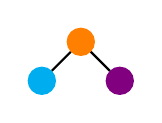
\begin{tikzpicture}[node distance={7mm}, thick, main/.style = {draw, circle, fill}]
			\node[main, color=cyan] (C) {};
			\node[main, color=orange] (O) [above right of=C] {};
			\node[main, color=violet] (V) [below right of=O] {};
			\draw (O) edge (V);
			\draw (C) edge (O);
		\end{tikzpicture}
		\caption{Corresponding graph.}
	\end{subfigure}
	\caption{Example of a graph from INT class.}
\end{figure}

\begin{figure}[!ht]\centering
	\begin{subfigure}{0.45\textwidth}\centering
		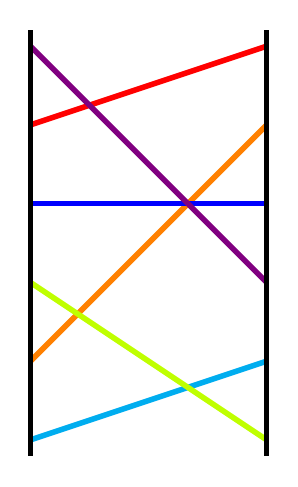
\begin{tikzpicture}[node distance={9mm}, thick, main/.style = {draw, circle}]
			\draw[line width = 2, color = cyan] (0,1) -- (3,2);
			\draw[line width = 2, color = orange] (0,2) -- (3,5);
			\draw[line width = 2, color = lime] (0,3) -- (3,1);
			\draw[line width = 2, color = blue] (0,4) -- (3,4);
			\draw[line width = 2, color = red] (0,5) -- (3,6);
			\draw[line width = 2, color = violet] (0,6) -- (3,3);
			\draw[line width = 2] (0,.8) -- (0,6.2);
			\draw[line width = 2] (3,.8) -- (3,6.2);
		\end{tikzpicture}
		\caption{Drawn permutations.}
	\end{subfigure}
	\begin{subfigure}{0.45\textwidth}\centering
		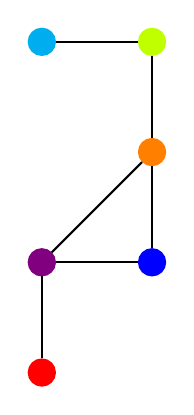
\begin{tikzpicture}[node distance={14mm}, thick, main/.style = {draw, circle, fill}]
			\node[main, color=cyan] (1) {};
			\node[main, color=lime] (2) [right of=1] {};
			\node[main, color=orange] (3) [below of=2] {};
			\node[main, color=blue] (4) [below of=3] {};
			\node[main, color=violet] (5) [left of=4] {};
			\node[main, color=red] (6) [below of=5] {};

			\draw (1) edge (2);
			\draw (2) edge (3);
			\draw (3) edge (4);
			\draw (3) edge (5);
			\draw (4) edge (5);
			\draw (5) edge (6);
		\end{tikzpicture}
		\caption{Corresponding graph.}
	\end{subfigure}
	\caption{Example of a graph from PER class.}
\end{figure}

\section{Chordal graphs}

\begin{defn}
	A graph is \textbf{chordal} if it does not contain any cycle of length greater than three as an induced subgraph.
\end{defn}

\begin{defn}
	A vertex $u$ of a graph $G$ is \textbf{simplicial} if $G[N_G(u)]$ is a clique.
\end{defn}

\begin{defn}[PES \PES]
	A \textbf{perfect elimination scheme} for a graph $G$ is a linear ordering $u_1, u_2, \dots, u_n$ of its vertices such that for every $i, u_i$ is simplicial in the induced subgraph $G[\{u_1, u_2, \dots, u_i\}]$.
\end{defn}

\begin{lemma}
	Every minimal vertex cut in a chordal graph induces a clique.
\end{lemma}

\begin{proof}
	Let $A \subset V(G)$ be a minimal vertex cut, and suppose $u, v$ be two vertices of $A$. These vertices	are connected by a path in each component of $G \setminus A$. If $u$ and $v$ were not adjacent, a pair of shortest such paths would give rise to an induced cycle of length greater than 3 in $G$.
\end{proof}

\begin{lemma}
	Every chordal graph, which is not a complete graph, contains two nonadjacent simplicial vertices.
	\label{lemma-r2}
\end{lemma}

\begin{proof}
	By induction. If $G$ is a complete graph, the claim of the lemma is fulfilled. If $G$ is not complete, it has a vertex cut, say $A$. Let $B$ be a connected component of $G \setminus A$, and set $G_1 = G[B \cup A]$ and $G_2 = G \setminus B$. By induction hypothesis, each of $G_1, G_2$ is either complete or has two nonadjacent simplicial vertices. Thus each of them has a simplicial vertex which does not belong to $A$. Each of	these is then also simplicial in entire $G$, and they are clearly nonadjacent.
\end{proof}

\begin{cor}
	Every nonempty chordal graph contains a simplicial vertex.
\end{cor}

\begin{defn}[Clique-tree decomposition]
	A \textbf{clique-tree decomposition} of a graph $G$ is a tree $T = (\mathcal{Q}, F)$, with $\mathcal{Q}$ being the set of all maximal cliques of $G$, such that for every vertex $u \in V(G)$, the subgraph $T[\{Q : u \in Q \in \mathcal{Q}\}]$ is connected.
\end{defn}

\textbf{Warning!! The vertex set of a clique-tree decomposition of a graph G is uniquely defined, but not necessarily the edge set!!}

\begin{thm}
	For any graph $G$, the following statements are equivalent:
	
	\begin{enumerate}
		\item $G$ is chordal,
		\item $G$ allows a PES.
		\item $G$ has a clique-tree decomposition, and
		\item $G$ is an intersection graph of subtrees of a tree.
	\end{enumerate}
\end{thm}

\begin{proof}
	"$1. \Rightarrow 2.$" By induction on the number of vertices, using Lemma \ref{lemma-r2}.
	
	"$2. \Rightarrow 3.$" By induction on the number of vertices again. Suppose $G' = G \setminus v_n$ has a clique-tree	$T = (\mathcal{Q}' , F')$. If $Q' = N_G (v_n) \in \mathcal{Q}'$ , then $Q = N_G [v_n]$ is a maximal clique in $G, \mathcal{Q} = (\mathcal{Q}' \setminus \{Q'\}) \cup \{Q\}$ and $T = (\mathcal{Q}, F)$ is a clique-tree for $G$, where $F = (F' \setminus \{Q' P : P \in \mathcal{Q}'\}) \cup \{QP : Q'P \in F'\}$. If, on the other hand, $Q' = N_G(v_n) \notin \mathcal{Q}'$ , then $\mathcal{Q} = \mathcal{Q}' \cup N_G [v_n]$ and $(\mathcal{Q}, F' \cup N_G [v_n]P)$ is a clique-tree for $G$ for any $P \in \mathcal{Q}'$ such that $N_G (v_n) \subset P$.
	
	"$3. \Rightarrow 4.$" Given a clique-tree decomposition $T = (\mathcal{Q}, F)$, define $T_u = T [\{Q : u \in Q \in \mathcal{Q}\}]$ for $u \in V(G)$. Clearly $V(T_u) \cap V(T_v) \neq \emptyset$ iff $u$ and $v$ belong to the same maximal clique of $G$, which happens if and only if $u$ and $v$ are adjacent in $G$.
	
	"$4. \Rightarrow 1.$" Let $G$ be the intersection graph of a collection $\{T_u\}_{u \in V(G)}$ of subtrees of a tree $T$. Suppose $v_1, v_2, \dots, v_k$ be an induced cycle in $G$, with $k > 3$. Then the subtrees $T_{v_1}$ and $T_{v_3}$ are vertex disjoint, and hence there is an edge $e \in E(T)$ which lies on every path connecting $T_{v_1}$ and $T_{v_3}$ in $T$ . This edge separates $T$ into $T_1$ and $T_2$ such that $T_{v_1}$ and $T_{v_3}$ belong to different components of $T \setminus e$, say, $T_{v_1} \subseteq T_1$ and $T_{v_3} \subseteq T_2$. One can show by induction on $i$ that for every $i \geq 3$, $T_{v_i} \subseteq T_2$. But then $T_{v_k}$ and $T_{v_1}$ must be disjoint, contradicting the assumption that $v_1 v_k \in E(G)$.
\end{proof}

\begin{cor}
	Chordal graphs are perfect (i.e., $\chi(H) = \omega(H)$ for every induced subgraph $H$ of $G$).
\end{cor}

\begin{proof}
	Consider a PES $u_1, u_2, \dots, u_n$ for $G$ and color the vertices from $u_1$ to $u_n$ by the First Fit Method (we try to use minimal color if we cannot use any of them, create a new color).
\end{proof}
	\chapter{Interval, permutation and function graphs}

\section{Interval graphs}

\begin{defn}
	A graph is an \textbf{interval graph} if it is isomorphic to the intersection graph of a collection of intervals on a line.
\end{defn}

\begin{observ}
	Every interval graph has an interval representation in which all of the intervals are closed.
\end{observ}

\begin{defn}[Clique-path decomposition]
	A \textbf{clique-path decomposition} of a graph is a clique-tree decompo-\newline sition in which the underlying tree is a path.
\end{defn}

\begin{thm}
	For any graph $G$, the following statements are equivalent:
	
	\begin{enumerate}
		\item $G$ is an interval graph,
		\item $G$ has a clique-path decomposition, and
		\item $G$ is an intersection graph of subpaths of a path.
	\end{enumerate}
\end{thm}

\begin{proof}
	"$1. \Leftrightarrow 3.$" is obvious.
	
	"$1. \Rightarrow 2.$" Assume $I_u , u \in V(G)$ is an interval representation of $G$. Use the fact that intervals on a line have the Helly property, i.e., if any two of a collection of intervals have a nonempty intersection, then all of them have a nonempty intersection. In other words, if $Q_i \in \mathcal{Q}$ is a maximal clique of $G$, then there exists a point $P_i$ which belongs to $\bigcap_{u \in Q_i} I_u$. Moreover, for every $v \notin Q_i , P_i \notin I_v$, since $Q_i$ is a maximal clique. (E.g., the rightmost of the left endpoints of the intervals $I_u , u \in Q_i$ is a good candidate for $P_i$.) Order the cliques of $Q$ as $Q_1, Q_2, \dots, Q_k$ so that $P_1 < P_2 < \dots < P_k$. Then the path
	$Q_1 Q_2 \dots Q_k$ is a clique-path decomposition of $G$.
	
	"$2. \Rightarrow 3.$" Given a clique-path decomposition $P = (\mathcal{Q}, F)$, define $P_u = P [\{Q : u \in Q \in \mathcal{Q}\}]$ for $u \in V(G)$. Clearly $V(P_u) \cap V(P_v) \neq \emptyset$ iff $u$ and $v$ belong to the same maximal clique of $G$, which happens if and only $u$ and $v$ are adjacent in $G$.
\end{proof}

\section{Comparability graphs}

\begin{defn}
	A graph $G$ is a \textbf{comparability graph} if there exists a partial order $P = (V(G), \leq)$ on the vertex set of $G$ (i.e., an \textbf{antireflexive}, \textbf{antisymmetric} and \textbf{transitive binary relation}) such that for any two vertices $u, v \in V(G)$, $uv \in E(G)$ if and only if $u \leq v$ or $v \leq u$ (i.e., if $u$ and $v$ are comparable in $P$). The class of comparability graphs will be denoted by CO.
\end{defn}

\begin{observ}
	A graph is a comparability graph if and only if its edges can be transitively oriented.
\end{observ}

\begin{thm}
	Comparability graphs are perfect.
\end{thm}

\begin{proof}
	Because $G \in CO$ then $\exists P = (V, \leq)$. We create a Haase diagram. Then we may see that cliques are chains and also independent sets are the antichains. Therefore we color every layer with one color and it is the same as the size of the largest clique.
\end{proof}

\begin{notation}
	If $\mathcal{A}$ is a graph class, the symbol $\text{co}-\mathcal{A}$ is used to denote the class containing the complements of the graphs in $\mathcal{A}$.
\end{notation}

\begin{observ}
	If $\mathcal{A} \subseteq \mathcal{B}$, then $\text{co}-\mathcal{A} \subseteq \text{co}-\mathcal{B}$.
\end{observ}

\begin{thm}
	All equivalencies hold:
	
	\begin{enumerate}
		\item $\text{FUN} = \text{co}-\text{CO}$
		\item $\text{PER} = \text{CO} \cap \text{co}-\text{CO}$
		\item $\text{INT} = \text{CHOR} \cap \text{co}-\text{CO}$
	\end{enumerate}
\end{thm}

\begin{proof}
	\begin{enumerate}
		\item ”FUN $\subseteq$ co-CO”: Given a collection of curves joining two vertical parallel lines (and lying in the stripe between them), for any two non-crossing curves, it is uniquely determined which one lies above the other one (this follows from the Jordan curve theorem), and this gives a transitive orientation of the complement of the intersection graph of this collection.
		
		”co-CO $\subseteq$ FUN”: Let $G = (V, E)$ be a graph and let $P = (V, \leq)$ be a partial order which corresponds to a transitive orientation of the complement of $G$. If $d$ is the dimension of $P$, $P$ is the intersection of $d$ linear orders $L_1, L_2 , \dots, L_d$ of $V$. In the plane, draw d distinct parallel (vertical) lines $l_1, l_2, \dots, l_d$, and on each $l_i$, mark distinct points $P_{iu}, u \in V$ bottom up in the order $L_i$. Consider piece-wise linear curves $c(u) = P_{1u} P_{2u} \dots P_{du}$, for $u \in V$. If $uv \in E$, $u$ and $v$ are incomparable in $P$,	and hence there are indices $i$ and $j$ such that $u <_{L_i} v$ and $v <_{L_j} u$, in other words $P_{iu}$ is below $P_{iv}$, while $P_{ju}$ is above $P_{jv}$. Hence the curves $c(u)$ and $c(v)$ cross somewhere between $l_i$ and $l_j$. If, on the other hand, $uv \notin E$, $uv$ is an edge of the complement of $G$ and hence $u$ and $v$ are comparable in $P$, say, $u \leq v$. But then $u <_{L_i} v$ for every $i = 1, 2, \dots, d$, and for each $i = 1, 2, \dots, d - 1$, the curve $c(u)$	lies below the curve $c(v)$ in the stripe between $l_i$ and $l_{i+1}$. Thus $c(u)$ and $c(v)$ are disjoint.
		
		\item Note first that co-PER $\subseteq$ PER. Indeed, given a permutation representation of a graph, swap	the order of the endpoints on one of the bounding lines to obtain a representation of the complement of the given graph. Then PER $=$ co-(co-PER) $\subseteq$ co-PER, and hence PER $=$ co-PER.
		
		”PER $\subseteq$ CO $\cap$ co-CO”: Obviously PER $\subseteq$ FUN $=$ co-CO. Then the above small observation implies PER $=$ co-PER $\subseteq$ co-(co-CO) $=$ CO as well.

		”CO $\cap$ co-CO $\subseteq$ PER”: Suppose both $G$ and its complement can be transitively oriented, say $\overrightarrow{E_1}$ be a transitive orientation of $G$ and $\overrightarrow{E_2}$ a transitive orientation of the complement $-G$ of $G$. Then $\overrightarrow{E_1} \cup \overrightarrow{E_2}$ is a transitive orientation of the complete graph $K_{V(G)}$ on the vertex set of $G$, i.e., a linear ordering of the vertices of $G$. And so is $\overrightarrow{E_1}^{-1} \cup \overrightarrow{E_2}$. Place the vertices of $G$ on two parallel lines, on one of them in the linear order given by $\overrightarrow{E_1} \cup \overrightarrow{E_2}$, on the other one in the order given by $\overrightarrow{E_1}^{-1} \cup \overrightarrow{E_2}$, and connect the two occurrences of a vertex $u$ by a straight-line segment called $s(u)$, for every vertex $u \in V(G)$. If $uv \in E(G)$, then the pair $u, v$ is ordered differently on the two lines (by $\overrightarrow{E_1}$ on one of them and by $\overrightarrow{E_1}^{-1}$ on the other one) and the segments $s(u), s(v)$ cross each other somewhere between	the two lines. If $uv \notin E(G)$, the pair $u, v$ is ordered the same way (by $\overrightarrow{E_2}$) on both of the lines, and thus the segments $s(u)$ and $s(v)$ are disjoint. So $\{s(u)\}_{u \in V(G)}$ is a permutation representation of $G$.
		
		\item ”INT $\subseteq$ CHOR $\cap$ co-CO”: Let $\{I(u)\}_{u \in V(G)}$ be an interval representation of a graph $G$. Define a transitive orientation $\overrightarrow{E_2}$ of the non-edges of $G$ by setting $uv \in \overrightarrow{E_2}$ if $\max I(u) < \min I(v)$. Thus $G \in$ co-CO. The fact that $G \in$ CHOR follows from the fact that
		
		$$
		\text{INT} = \mathcal{IG}(\{\text{connected subgraphs of paths}\}) \subseteq
		$$
		
		$$
		\subseteq \mathcal{IG}(\{\text{connected subgraphs of trees}\}) = \text{CHOR}.
		$$
		
		”CHOR $\cap$ co-CO $\subseteq$ INT”: Let $G$ be a chordal graph which allows a transitive orientation $\overrightarrow{E_2}$ of its non-edges. Define a binary relation $<$ on the set $\mathcal{Q}$ of maximal cliques of $G$ by setting
		
		$$
		Q < Q' \Leftrightarrow \exists u \in Q \exists v \in Q' : uv \in \overrightarrow{E_2}.
		$$
		
		\begin{claim}
			The relation $<$ is a partial order on $\mathcal{Q}$.
		\end{claim}
		
		\begin{proof}[Proof of claim]
			We will show all properties of partial order.
			\begin{itemize}
				\item Antireflexivity: Each $Q \in \mathcal{Q}$ is a clique, so there are no two vertices $u, v \in Q$ that would form a	non-edge of $G$. Hence $Q \not< Q$.
				
				\item Antisymmetry: Suppose for the contrary that there are $u \in Q, v \in Q'$ s.t. $uv \in \overrightarrow{E_2}$, and another pair $x \in Q, y \in Q'$ s.t. $yx \in \overrightarrow{E_2}$. First observe that $u \neq x$ and $v \neq y$ (if $u = x$, the transitivity of $\overrightarrow{E_2}$ would imply $yv \in \overrightarrow{E_2}$, which is impossible; if $v = y$, the transitivity of $\overrightarrow{E_2}$ would imply $ux \in \overrightarrow{E_2}$, which is again impossible). Next observe that both $uy$ and $xv$ must be edges of $G$ (if $uy \notin E(G)$, then either $uy \in \overrightarrow{E_2}$, or $yu \in \overrightarrow{E_2}$, yielding $ux \in \overrightarrow{E_2}$ in the former case and $yv \in \overrightarrow{E_2}$ in the letter one, both contradicting the fact that $Q$ and $Q'$ are cliques of $G$; the case of $xv \notin E(G)$ is analogous). Lastly, we conclude that $G[\{u, v, x, y\}] \simeq C_4$ , contradicting the assumption that $G$ is chordal.
				
				\item Transitivity: Suppose $Q < Q' < Q''$ and let $u \in Q, v, x \in Q'$ and $y \in Q''$ be vertices such that $uv, xy \in \overrightarrow{E_2}$. If $v = x$, the transitivity of $\overrightarrow{E_2}$ implies $uy \in \overrightarrow{E_2}$, hence $Q < Q''$. If $v \neq x$, one of $ux$, $vy$
				must be a non-edge (otherwise $G[\{u, v, x, y\}]$ would be an induced cycle of length 4, contradicting the assumption that $G$ is chordal). If $ux \notin E(G)$, $ux \in \overrightarrow{E_2}$ and the transitivity of $\overrightarrow{E_2}$ implies $uy \in \overrightarrow{E_2}$. If $vy \notin E(G)$, $vy \in \overrightarrow{E_2}$ and the transitivity of $\overrightarrow{E_2}$ implies $uy \in \overrightarrow{E_2}$. In either case, $Q < Q''$.
			\end{itemize}
		\end{proof}
		
		\begin{claim}
			The relation $<$ is a linear ordering of $\mathcal{Q}$.
		\end{claim}
		
		\begin{proof}[Proof of claim]
			Let $Q \neq Q'$ be two different maximal cliques of $G$. Their maximality implies that none of them is a subset of the other one. Hence there is a vertex $u \in Q$ which does not belong to $Q'$ . If $u$ were adjacent to all vertices of $Q'$, $Q' \cup \{u\}$ would be a clique of $G$, contradicting the maximality of $Q'$ . Hence there is a $v \in Q'$ such that $uv \notin E(G)$. Then either $uv \in \overrightarrow{E_2}$ or $vu \overrightarrow{E_2}$, thus $Q < Q'$ or $Q' < Q$.
		\end{proof}
		
		\begin{claim}
			Let $\mathcal{Q} = \{Q_1 < Q_2 < \dots < Q_k\}$ be the maximal cliques of $G$ ordered by $<$. Then $P_G = (\mathcal{Q}, \{Q_i Q_{i+1}: i = 1, 2, \dots, k - 1\})$ is a clique-path decomposition of $G$, and hence $G \in$ INT.
		\end{claim}
		
		\begin{proof}[Proof of claim]
			Indeed $P_G$ is a path whose nodes are the maximal cliques of $G$. It remains to show that vertices of $G$ appear in these cliques consecutively. Suppose $Q < Q' < Q''$ and $u \in Q \cap Q''$. If there were a vertex $v \in Q'$ nonadjacent to $u$, we would have $uv \in \overrightarrow{E_2}$ because of $Q < Q'$ and $vu \in \overrightarrow{E_2}$ because of $Q' < Q''$, contradicting the antisymmetry of $\overrightarrow{E_2}$. Hence $u$ is adjacent to all vertices of $Q'$ , and thus
			$u \in Q'$ follows from the maximality of $Q'$.
		\end{proof}
	\end{enumerate}
	
	The last claim proved the theorem as well.
\end{proof}
	\chapter{Interval filament graphs}

\begin{defn}
	Given a half-plane $\pi$ with a border-line $l$, an \textbf{interval filament} in $\pi$ is a simple curve with endpoints on $l$, its interior lying in $\pi$ and within the stripe determined by lines perpendicular to $l$ and passing through the endpoints of the curve. The class of \textbf{interval filament graphs} is $\text{IFA} = \mathcal{IG}\{$interval filaments in a half-plane$\}$.
\end{defn}

\begin{figure}[!ht]\centering
	\begin{tikzpicture}
		\draw[color = gray] (2,0) -- (10,0);
		\node at (3,.3) {$l$};
		\draw[color=black, thick] (5,.01) edge (10,.01);
		\draw[dotted] (5,0) edge (5, 5);
		\draw[dotted] (10,0) edge (10,5);
		
		\draw[color=Red, thick] (5, .01) .. controls (10,5) and (4,3) .. (7, 4);
		\draw[color=Red, thick] (7, 4) .. controls (11,1) and (1,1) .. (10, .01);
		
		\fill[color=Red] (7,4) circle[radius=.35pt];
	\end{tikzpicture}
	\caption{An illustration to the definition. The name “interval-filament” comes from the fact that the curve “lives above” the interval that is determined by the endpoints of the filament on the boundary line $l$.}
\end{figure}

\begin{comm}
	If the base intervals of two interval-filaments overlap (i.e., they are not disjoint, but none of them is a subinterval of the other one), the filaments necessarily cross each other and the corresponding vertices in the intersection graph are adjacent (cf. the blue and red filaments in Fig. \ref{filaments}). On the other hand, if one of the base intervals is included in the other one, their filaments may or may not be disjoint (cf. the blue and yellow filaments for the disjoint case, and the red and green filaments for the non-disjoint one, both in Fig. \ref{filaments}).
\end{comm}

\begin{figure}[!ht]\centering
	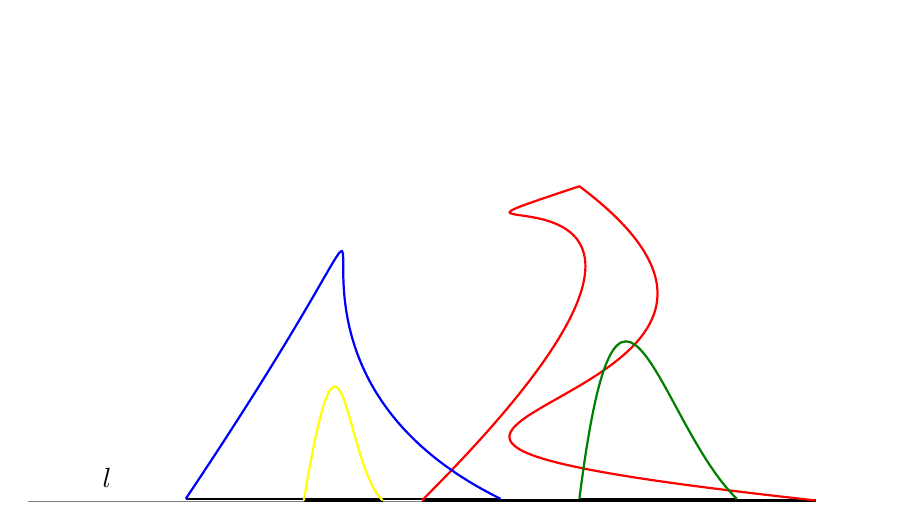
\begin{tikzpicture}
		\draw[color = gray] (0,0) -- (10,0);
		\node at (1,.3) {$l$};
		
		\draw[color=black, thick] (5,.01) edge (10,.01);
		\draw[color=black, thick] (7,.03) edge (9,.03);
		\draw[color=black, thick] (2,.03) edge (6,.03);
		\draw[color=black, thick] (3.5,.01) edge (4.5,.01);
		
		\draw[color=Red, thick] (5, .01) .. controls (10,5) and (4,3) .. (7, 4);
		\draw[color=Red, thick] (7, 4) .. controls (11,1) and (1,1) .. (10, .01);
		\fill[color=Red] (7,4) circle[radius=.35pt];
		
		\draw[color=Yellow, thick] (3.5, .01) .. controls (4,3) and (4,.5) .. (4.5, .01);
		\draw[color=Blue, thick] (2, .03) .. controls (6,6) and (2,2) .. (6, .03);
		\draw[color=Green, thick] (7, .03) .. controls (7.5,4) and (8,1) .. (9, .03);
	\end{tikzpicture}
	\caption{An illustration to the possible relative positions of interval-filaments.}
	\label{filaments}
\end{figure}

\begin{observ}
	$\text{IFA}$ contains $\text{INT}$, $\text{CHOR}$, $\text{FUN}$, $\text{CIR}$, $\text{CA}$, and $\text{PC}$.
\end{observ}

\begin{defn}[class $\mathcal{A}$-mixed]
	Let $\mathcal{A}$ be a graph class. A graph $G = (V, E)$ belongs to the class $\mathcal{A}$-mixed if its edge set allows a partition $E = E_1 \cup E_2$ and a transitive orientation $\overrightarrow{E_2}$ of $E_2$ such that for any three vertices $u, v, w \in V(G)$, $uv \in \overrightarrow{E_2}$ and $vw \in E_1$ imply $uw \in E_1$.
\end{defn}

\begin{thm}
	co-IFA = (co-INT)-mixed.
\end{thm}

\begin{proof}
	"$\subseteq$": Let $G = (V, E) \in \text{IFA}$ and let $\{f_u : u \in V\}$ be an interval-filament representation of $G$, with $f_u$ being a filament with its base interval $I_u$ lying on a common line $l$. Then its complement $-G$ is in co-IFA, and our goal is to show that $-G \in$ (co-INT)-mixed. Define
	
	$$
	E_1 = \{uv : I_u \cap I_v = \emptyset\}
	$$
	
	and
	
	$$
	E_2 = \{uv : ((I_u \subseteq I_v ) \lor (I_v \subseteq I_u )) \land (f_u \cap f_v = \emptyset)\}.
	$$
	
	Then
	$$
	\overrightarrow{E_2} = \{uv : (I_u \subseteq I_v ) \land (f_u \cap f_v = \emptyset)\}
	$$
	
	is a transitive orientation of $E_2$, $E_1 \cup E_2 = \binom{V}{2} \setminus E$, $(V, E_1) \in$ co-INT and $E_1$ and $\overrightarrow{E_2}$ satisfy the mixing property. Hence $-G \in$ (co-INT)-mixed.
	
	"$\supseteq$": Consider a graph in (co-INT)-mixed and denote its complement by $G = (V, E)$. Our goal is to show that $-G \in$ co-IFA, or equivalently that $G \in$ IFA. Since $-G$ is (co-INT)-mixed, the non-edges of $G$ can be partitioned into disjoint sets $E_1$, $E_2$ so that $G_1 = (V, E_1) \in$ co-INT, and $E_2$ allows a transitive orientation $\overrightarrow{E_2}$ such that $E_1$ and $\overrightarrow{E_2}$ satisfy the mixing property. Fix this partition $E_1$, $E_2$ and the transitive orientation $\overrightarrow{E_2}$.
	
	Consider an interval intersection representation $\mathcal{R} = \{I_u = [l_u , r_u] : u \in V\}$ of $-G_1$ . We will only consider representations in which all end-points of the intervals are different points on the base line. For two vertices $u, v \in V$, there are three possibilities for the relative position of the intervals $I_u$, $I_v$ -- the intervals are disjoint (when $r_u < l_v$ or $r_v < l_u$), or in inclusion (when $l_u < l_v < r_v < r_u$ or $l_v <
	l_u < r_u < r_v$), or overlapping (when $l_u < l_v < r_u < r_v$ or $l_v < l_u < r_v < r_u$). Given a representation	$\mathcal{R}$, we set $\mathcal{R}_{\text{disjoint}} = \{uv : I_u \text{ and } I_v \text{ are disjoint}\}$, $\mathcal{R}_{\text{inclusion}} = \{uv : I_u \text{ and } I_v \text{ are in inclusion}\}$ and $\mathcal{R}_{\text{overlap}} = \{uv : I_u \text{ and } I_v \text{ are overlapping}\}$. Observe that $\mathcal{R}$ is an interval intersection representation of $-G_1$ if and only if $\mathcal{R}_{\text{disjoint}} = E_1$. In such a case, $\mathcal{R}_{\text{inclusion}} \cup \mathcal{R}_{\text{overlap}} = E \cup E_2$.
	
	\begin{figure}[!ht]\centering
		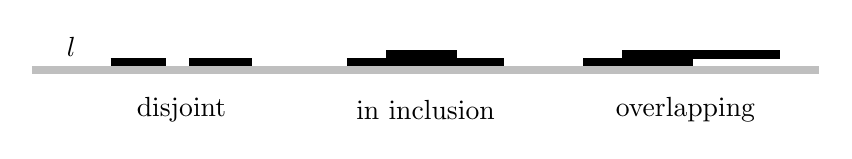
\begin{tikzpicture}
			%% Lines
			\draw[line width = 3, color=lightgray] (0,0) -- (10,0);
			% Disjoint
			\draw[line width = 3, color=black] (1,.10) -- (1.7,.10);
			\draw[line width = 3, color=black] (2,.10) -- (2.8,.10);
			% In inclusion
			\draw[line width = 3, color=black] (4,.10) -- (6,.10);
			\draw[line width = 3, color=black] (4.5,.20) -- (5.4,.20);
			% Overlaping
			\draw[line width = 3, color=black] (7,.10) -- (8.4,.10);
			\draw[line width = 3, color=black] (7.5,.20) -- (9.5,.20);
			%% Text boxes
			\node (l) at (.5,.3) {$l$};
			\node (disjoint) at (1.9, -.5) {disjoint};
			\node (incl) at (5, -.5) {in inclusion};
			\node (overlap) at (8.3, -.5) {overlapping};
		\end{tikzpicture}
		\caption{An illustration to the possible relative positions of pairs of intervals.}
	\end{figure}
	
	\begin{claim}
		If $E_1$ and $E_2$ satisfy the mixing condition, $-G_1$ has an interval intersection representation such that for every two vertices $u, v \in V$, $uv \in \overrightarrow{E_2}$ implies $I_u \subseteq I_v$.
	\end{claim}
	
	\begin{proof}[Proof of claim]
		Let us call a violation a pair of endpoints of intervals $I_u$, $I_v$ with $uv \in \overrightarrow{E_2}$ such that $l_u < l_v$ or $r_v < r_u$. Observe that overlapping intervals provide one violation, while intervals in inclusion provide either $0$ (when $I_u \subseteq I_v$) or $2$ (when $I_v \subseteq I_u$) violations.
		
		Consider a representation $\mathcal{R}$ with the smallest possible number of violations. We will prove that
		this number is zero, i.e., that this $\mathcal{R}$ satisfies the statement of the Claim.
		
		Suppose, for the contrary, that $\mathcal{R}$ has $k > 0$ violations. For every violation, count the number of endpoints of other intervals lying between the two endpoints forming this violation, and let $m$ be the minimum of these counts over all violations. Assume that $\mathcal{R}$ is chosen such that $m$ is minimum possible among all representations with $k$ violations. In the case analysis which follows, we assume that the violation achieving this minimum number of endpoints is formed by the right endpoints of $I_u$ and $I_v$. If it is achieved by their left endpoints, the arguments are similar (and symmetric).
		
		\begin{itemize}[]
			\item \underline{Case $B1$. $m = 0$} Let $r_v < r_u$, with $uv \in \overrightarrow{E_2}$, be a violation such that there are no other endpoints between $r_v$ and $r_u$. Change the representation $\mathcal{R}$ to $\mathcal{R}'$ by changing the interval $I_v$ to $I_v' = [l_v , r_u + \epsilon]$ for a positive $\epsilon$ small enough so that no endpoint of any interval is between $r_u$ and $r_u + \epsilon$ (other intervals remain the same as in $\mathcal{R}$). Then $\mathcal{R}'$ is still an interval intersection representation of $-G_1$, but it has $k - 1 < k$ violations, contradicting the assumption that $k$ was the minimum possible number of violations in an interval representation of $-G_1$.
			
			\item \underline{Case $B2$. $m > 0$} Let $r_v < r_u$, with $uv \in \overrightarrow{E_2}$, be a violation with $m$ endpoints between $r_v$ and $r_u$. Let $P$ be the leftmost of these endpoints.
			
			\begin{itemize}[]
				\item \underline{Subcase $B2\alpha$. $P$ is the right endpoint of an interval.} Let $w \in V$ be such that $P = r_w$. Change the represen-\newline tation $\mathcal{R}$ to $\mathcal{R}'$ by changing the interval $I_v$ to $I_v' = [l_v , r_w + \epsilon]$ for a positive $\epsilon$ small enough so that no endpoint of any interval is between $r_w$ and $r_w + \epsilon$. Then $\mathcal{R}'$ is still an interval intersection representation of $-G_1$. The number of endpoints between $r_v'$ and $r_u$ is $m - 1 < m$. If $\mathcal{R}'$ had the same number of violations as $\mathcal{R}$, this would contradict the assumption of minimality of $m$. Thus $\mathcal{R}'$ must have more than $k$ violations. The only new violation can be formed by $r_w < r_v'$, which means that $vw \in \overrightarrow{E_2}$. Then the transitivity of $\overrightarrow{E_2}$ implies that $uw \in \overrightarrow{E_2}$ and $r_w < r_u$ is a violation in $\mathcal{R}$ with $m - 1 < m$ endpoints between $r_w$ and $r_u$, contradicting the assumption on minimality of $m$.
				
				\item \underline{Subcase $B2\beta$. $P$ is the left endpoint of an interval.} Let $w \in V$ be such that $P = l_w$. Then $I_v \cap I_w = \emptyset$ and hence $vw \in E_1$. The mixing property applied to $u, v, w$ then implies $uw \in E_1$, which is impossible since $P \in I_u \cap I_w \neq \emptyset$.
			\end{itemize}
		\end{itemize}
		
		Thus both Cases $B2$ and $B1$ lead to contradictions, and hence $k = 0$ and $\mathcal{R}$ satisfies the property described in the Claim.
	\end{proof}
	
	Assume we are having an interval intersection representation $\mathcal{R}$ guaranteed by the Claim. It follows that $E_2 \subseteq \mathcal{R}_\text{inclusion}$, and hence $\mathcal{R}_\text{overlap} \subseteq E$. In the first step, define, for every vertex $u \in V$, the interval filament $f_u$ as the half-circle with diameter $I_u$. At this point we observe the following
	
	\begin{enumerate}
		\item if $I_u$ and $I_v$ are disjoint, so are also $f_u$ and $f_v$, which corresponds to the fact that $uv \in E_1$ and thus $uv \notin E$;
		\item if $I_u$ and $I_v$ are overlapping, $f_u$ and $f_v$ cross each other, which corresponds to the fact that $uv \in E$ which is observed above; however
		\item if $I_u$ and $I_v$ are in inclusion, say $I_u \subseteq I_v$, then either $uv \in E_2$ (and thus $uv \in \overrightarrow{E_2}$) or $uv \in E$, but $f_u \cap f_v = \emptyset$ in both cases.
	\end{enumerate}
	
	We will now modify some of the filaments in order to make filaments of case 3 intersect if the corresponding vertices are adjacent in $G$. For every pair of vertices $u, v \in V$ such that $I_u \subseteq I_v$ and $uv \in E$, choose a line $l_u$ perpendicular to the base line $l$ and crossing it in an interior point of $I_u$. Then pull the filament $f_u$ up along $l_u$ to make it cross $f_v$ (cf. an illustrative Fig. \ref{left}). To avoid creating undesired intersections with other filaments, we must modify also those filaments which cross the line $l_u$ between its crossings with $f_u$ and $f_v$. Imagine this as a dynamic process, as if $f_u$ would slowly grow a spike upward and this spike would be pushing every filament $f_w$ in front of it, if $w$ is such that $uw \notin E$. Moreover, if there were another filament $f_z$ above $f_w$ such that $wz \notin E$, $f_z$ would be pushed by $f_w$ etc. See Fig. \ref{right}. We claim that in this way no undesired intersections arise. Such could be only between one of the pushed filaments, say $f_y$, and the filament $f_v$. If $f_y$ is pushed, there is a sequence of vertices $u_0 = u, u_1 , \dots , u_t = y$ such that $f_{u_{i-1}}$ pushes $f_{u_{i}}$ for $i = 1, 2, \dots , t$, i.e., $u_{i-1} u_i \notin E$	and $I_{u_{i-1}} \subseteq I_{u_{i}}$, hence $u_{i-1} u_i \in \overrightarrow{E_2}$. Transitivity of $\overrightarrow{E_2}$ then implies $uy \in \overrightarrow{E_2}$. Similarly, if $f_y$ should not cross $f_v$, i.e., $yv \notin E$, we would have $yv \in \overrightarrow{E_2}$. But that would imply $uv \in \overrightarrow{E_2}$ contradicting the assumption that $uv \in E$.
	
	\begin{figure}[!ht]\centering
		\begin{subfigure}{0.45\textwidth}\centering
			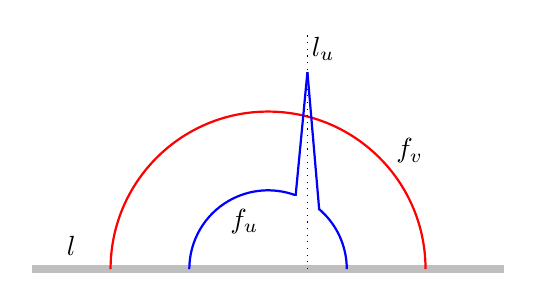
\begin{tikzpicture}
				%% Lines
				\draw[line width = 3, color=lightgray] (0,0) -- (6,0);
				\draw[color=Red, thick] (1,0) arc (180:0:2);
				\draw[color=Blue, thick] (2,0) arc(180:70:1);
				\draw[color=Blue, thick] (4,0) arc(-180:-130:-1);
				\draw[dotted] (3.5, 0) -- (3.5, 3);
				\draw[color=Blue, thick] (3.35,0.93) -- (3.5, 2.5);
				\draw[color=Blue, thick] (3.65,0.75) -- (3.5, 2.5);
				%% Text boxes
				\node (l) at (.5,.3) {$l$};
				\node (lu) at (3.7,2.8) {$l_u$};
				\node (fv) at (4.8,1.5) {$f_v$};
				\node (fu) at (2.7,.6) {$f_u$};
			\end{tikzpicture}
			\caption{Crossing filaments.}
			\label{left}
		\end{subfigure}
		\begin{subfigure}{0.45\textwidth}\centering
			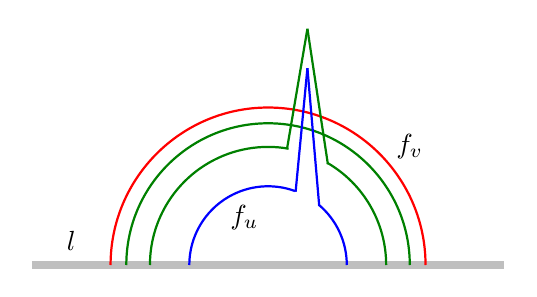
\begin{tikzpicture}
				%% Lines
				\draw[line width = 3, color=lightgray] (0,0) -- (6,0);
				\draw[color=Red, thick] (1,0) arc (180:0:2);
				
				\draw[color=Green, thick] (1.2,0) arc (180:0:1.8);
				
				\draw[color=Blue, thick] (2,0) arc(180:70:1);
				\draw[color=Blue, thick] (4,0) arc(-180:-130:-1);
				\draw[color=Blue, thick] (3.35,0.93) -- (3.5, 2.5);
				\draw[color=Blue, thick] (3.65,0.75) -- (3.5, 2.5);
				
				\draw[color=Green, thick] (1.5,0) arc(180:80:1.5);
				\draw[color=Green, thick] (4.5,0) arc(-180:-120:-1.5);
				\draw[color=Green, thick] (3.24,1.47) -- (3.5, 3);
				\draw[color=Green, thick] (3.76,1.28) -- (3.5, 3);
				%% Text boxes
				\node (l) at (.5,.3) {$l$};
				\node (fv) at (4.8,1.5) {$f_v$};
				\node (fu) at (2.7,.6) {$f_u$};
			\end{tikzpicture}
			\caption{Pushing outwards.}
			\label{right}
		\end{subfigure}
		\caption{Final modification of interval-filaments in the representation.}
	\end{figure}
\end{proof}
	\chapter{Cliques and independent sets}

We will show the computational complexity of the following optimization problems:

\begin{itemize}[]
	\item \textbf{Clique}
	\item \textit{Input:} A graph $G$.
	\item \textit{Output:} $\omega(G)$.
\end{itemize}

and

\begin{itemize} []
	\item \textbf{Independent Set}
	\item \textit{Input:} A graph $G$.
	\item \textit{Output:} $\alpha(G)$.
\end{itemize}

and their weighted variants

\begin{itemize}[]
	\item \textbf{Weighted Clique}
	\item \textit{Input:} A graph $G$ and a non-negative weight function $w : V(G) \to \R_0^+$.
	\item \textit{Output:} A clique $C \subseteq V(G)$ which maximizes $w(C) = \sum_{u \in C} w(u)$.
\end{itemize}

and

\begin{itemize}[]
	\item \textbf{Weighted Independent Set}
	\item \textit{Input:} A graph $G$ and a non-negative weight function $w : V(G) \to \R_0^+$.
	\item \textit{Output:} An independent set $A \subseteq V(G)$ which maximizes $w(A) = \sum_{u \in A} w(u)$.
\end{itemize}

Our goal is to show that for many of the intersection-defined graph classes that we have seen so far, these problems can be solved in polynomial time. For the sake of brevity, we denote by $\omega_w(G)$ the maximum possible weight $w(C)$ over all cliques $C$ in $G$, and by $\alpha_w(G)$ the maximum possible weight $w(A)$ over all independent sets $A$ in $G$.

\section{Interval graphs}

\begin{thm}
	\textbf{Weighted Clique} can be solved in polynomial time for interval graphs.
\end{thm}

\begin{proof}
	Interval graphs have only linearly many maximal cliques. We look at all of them and compare
	their weights.
\end{proof}

\begin{thm}
	\textbf{Weighted Independent Set} can be solved in polynomial time for interval graphs.
\end{thm}

\begin{proof}
	Suppose we are given an interval intersection representation $\mathcal{R} = \{I_u = [l_u , r_u] : u \in V\}$ of	a graph $G = (V, E)$, equipped with a weight function $w$. We may assume that all endpoints of the intervals are different. Number the endpoints $P_1 , P_2 , \dots , P_{2n}$ so that $P_i < P_{i+1}$ for $i = 1, 2, \dots , 2n - 1$.	Use dynamic programming to compute $w_i$ which is defined as the maximum possible weight of an	independent set $A$ in $G$ such that $r_u < P_i$ for all $u \in A$. This can be computed as follows:
	
	\begin{algorithm}[!ht]
		\begin{algorithmic}[1]
			\State $w_i := 0$
			\For{$i := 1$ to $2n$}
				\If{$P_i$ is the left endpoint of an interval}
					\State $w_{i+1} := w_i$
				\Else
					\State let $u \in V$ be such that $r_u = P_i$ and let $j$ be such that $P_j = l_u$;
					\State set $w_{i+1} = \max \{w_j + w(u), w_i\}$
				\EndIf
			\EndFor
			\State \Return $w_{2n+1}$
		\end{algorithmic}
	\end{algorithm}
\end{proof}

\begin{cor}
	\textbf{Weighted Clique} and \textbf{Weighted Independent Set} can both be solved in polynomial	time on co-INT graphs.
\end{cor}

\section{Comparability graphs}

\begin{thm}
	\textbf{Weighted Clique} can be solved in polynomial time for comparability graphs.
\end{thm}

\begin{proof}
	Given a transitive orientation $\overrightarrow{E}$ of $G = (V, E)$, order the vertices linearly $V = \{v_1 , v_2 , \dots, v_n\}$ in a topological sorting according to $\overrightarrow{E}$ (i.e., $v_i v_j \in \overrightarrow{E}$ implies $i < j$). For each $i$, set $W_i = \{j : v_j v_i \in E\}$ and let $w_i$ be the maximum weight $w(C)$ over all cliques $C \subseteq W_i \cup \{v_i\}$. Note that if $w(v_i) > 0$, each clique attaining the maximum weight contains $v_i$, and we may consider without loss	of generality only the cliques that contain $v_i$ even if $w(v_i) = 0$. The values $w_i , i = 1, 2, \dots , n$ can be computed recursively as follows
	
	\begin{algorithm}[!ht]
		\begin{algorithmic}[1]
			\For{$i := 1$ to $n$}
				\State $w_i := \max_{j \in W_i} w_j + w(v_i)$
			\EndFor
		\end{algorithmic}
	\end{algorithm}
	
	and clearly $\omega_w(G) = max_{i=1}^n w_i$.
\end{proof}

\begin{thm}
	\textbf{Weighted Independent Set} can be solved in polynomial time for \\ comparability graphs.
	\label{thm-4}
\end{thm}

\begin{proof}
	Given a transitive orientation $\overrightarrow{E}$ of $G = (V, E)$, consider the partial order $P = (V, \overrightarrow{E})$ determined by this orientation. The weighted version of Dilworth theorem yields that $\alpha_w(P)$ is equal to the minimum cost of a flow in the network $N = (V \cup \{s, t\}, E \cup \{su, ut : u \in V\})$ with vertex demands $f(u) \geq w(u)$, and this can be computed in polynomial time by network flow algorithms.
\end{proof}

\begin{cor}
	\textbf{Weighted Clique} and \textbf{Weighted Independent Set} can both be solved in polynomial time on function (= co-comparability) graphs.
\end{cor}

\section{Interval-filament graphs}

In this section we show the strongest results. Note, however, that we need the input graph to be given with an interval-filament representation (or, equivalently, with a partition of its edge set satisfying the mixing property).

\begin{thm}
	\textbf{Weighted Clique} can be solved in polynomial time for interval-filament graphs, if an interval-filament representation is provided on the input.
\end{thm}

\begin{proof}
	Suppose $\mathcal{R} = \{f_u : u \in V \}$ is an interval-filament representation of $G$, with $I_u$ being the base	interval of the filament $f_u$ for each $u \in V$, and let $w$ be the input weight function. We may suppose that the endpoints of the base intervals are mutually distinct, and we number them $P_1 , P_2 , \dots , P_{2n}$ from left to right. We further introduce points $Q_1 , Q_2 , \dots , Q_{2n-1}$ so that $Q_i$ lies between $P_i$ and $P_{i+1}$ for $i = 1, 2, \dots, 2n - 1$. Set $V_i = \{u : Q_i \in I_u\}$. If $C \subseteq V$ is a clique in $G$, the intervals $I_u$, $u \in C$ have a non-empty intersection, and hence $C \subseteq V_i$ for some $i$. Thus $\omega_w(G) = max_{i=1}^{2n-1} \omega_w (G[V_i])$ and each $\omega_w (G[V_i])$ can be computed in polynomial time by Theorem \ref{thm-4} since $G[V_i]$ is a co-comparability graph.
\end{proof}

\begin{thm}
	Suppose \textbf{Weighted Clique} can be solved in polynomial time for graphs from a	hereditary graph class $\mathcal{A}$. Then it can be solved in polynomial time for $\mathcal{A}$-mixed graphs, provided a partition of the edges of the input graph that satisfies the mixing property is a part of the input.
	\label{thm-6}
\end{thm}

\begin{proof}
	Given a graph $G = (V, E)$, a weight function $w \to \R_0^+$ and a partition $E = E_1 \cup E_2$ such that $(V, E_1) \in \mathcal{A}$, together with a transitive orientation $\overrightarrow{E_2}$ of $E_2$ which satisfies the mixing property, order the vertices $V = \{v_1 , v_2 , \dots , v_n\}$ in a topological sorting with respect to $\overrightarrow{E_2}$. For every vertex $v_i \in V$, set $W_i = \{v_j : v_j v_i \in \overrightarrow{E_2}\}$. Let $w_i = \omega_w (G[W_i \cup \{v_i\}])$ and let $C_i$ be a clique in $G[W_i \cup \{v_i\}]$ of weight $w_i$.
	
	\begin{claim}
		Let $M \subseteq W_i$ be a maximum weighted clique in the graph $(W_i , E_1 \cap \binom{W_i}{2})$ with respect to the weight function $\bar{w}(v_j) = w_j$ for $v_j \in W_i$. Then
		
		$$
		C = \bigcup_{v_j \in M} C_j \cup \{v_i\}
		$$
		
		is a maximum weighted clique in $G[W_i \cup \{v_i\}]$ with respect to $w$ and its weight is $w_i = \sum_{j: v_j \in M} w_j + w(v_i)$.
	\end{claim}
	
	\begin{proof}[Proof of claim]
		First we show that $C$ is a clique. Due to transitivity of $\overrightarrow{E_2}$, for every $v_j \in M$ and every $x \in C_j$, $xv_i \in \overrightarrow{E_2}$, and hence $xv_i \in E_2 \subseteq E$. Hence $C$ is a clique if $|M| = 1$. If $|M| > 1$, consider $v_j, v_h \in M$ and $x \in C_j$, $y \in C_h$. Suppose $x \neq v_j$. The mixing property, when applied to $x, v_j , v_h$, then implies $xv_h \in E_1$. If $y \neq v_h$, the mixing property, when applied to $y, v_h , x$, implies $yx \in E_1$. These situations cover all pairs of vertices in $C$.
		
		Next we show that any two $C_j$, $C_h$ are disjoint. If there were an $x \in C_j \cap C_h$, this $x$ would be different from both $v_j$ and $v_h$. But then $xv_j \in \overrightarrow{E_2}$ and $v_j v_h \in E_1$ imply (via the mixing property) $xv_h \in E_1$, contradicting the assumption $x \in C_h$. It further follows that $w(C) = \sum_{j:v_j \in M} \sum_{x \in C_j} w(x) + w(v_i) = \sum_{j:v_j \in M} w_j + w(v_i)$.
		
		Finally we show that the weight of $C$ is maximum possible. Suppose $D \subseteq W_i \cup \{v_i\}$ is a clique in $G[W_i \cup \{v_i\}]$ of maximum weight with respect to $w$. Obviously $v_i \in D$. Denote $\bar{D} = D \setminus \{v_i\}$ and consider $\bar{G} = (\bar{D}, \overrightarrow{E_2} \cap \bar{D} \times \bar{D})$. This $\bar{G}$ is an acyclic graph. Denote by $\bar{M}$ the sinks of $\bar{G}$. Every other vertex of $\bar{D}$ is connected to some vertex of $\bar{M}$ by a directed path, and hence, due to transitivity of $\overrightarrow{E_2}$, by a directed edge from $\overrightarrow{E_2}$. Set $\bar{D}_j = \{u : uv_j \in \overrightarrow{E_2} \land u \in \bar{D}\}$ and $D_j = \bar{D}_j \cup \{v_j\}$, for $v_j \in \bar{M}$. The mixing property implies that for $j \neq h$, $D_j \cap D_h = \emptyset$. Since $D_j$ is a clique in $G[W_j \cup \{v_j\}]$, it is $w(D_j) \leq w_j = \bar{w}(v_j)$. All vertices of $\bar{M}$ are sinks of $\bar{G}$, and thus any two of them are connected by an edge of $E_1$. Hence $M$ is a clique in $(W_i , E_1 \cap \binom{W_i}{2})$, and therefore $\bar{w}(\bar{M}) \leq \bar{w}(M)$. Thus
		
		$$
		\begin{aligned}
			w(D) &= w(v_i) + \sum_{j: v_j \in \bar{M}} \sum_{x \in D_j} w(x) = w(v_i) + \sum_{j:v_j \in \bar{M}} w(D_j) \leq w(v_i) + \sum_{j:v_j \in \bar{M}} \bar{w}(v_j)\\
			& = w(v_i) + \bar{w}(\bar{M}) \leq w(v_i) + \bar{w}(M) = w(C)
		\end{aligned}
		$$
		
		and $C$ is indeed a maximum weighted clique with respect to the weight function $w$.
	\end{proof}
	
	Having proved the observations above, we can now summarize the algorithm for finding a maximum weighted clique in an $\mathcal{A}$-mixed graph. Note that the preprocessing trick with adding a dummy vertex $v_{n+1}$ is introduced for the comfort of a more succinct write-up of the algorithm.
	
	\begin{algorithm}[!ht]
		\caption{Weighted Clique in $\mathcal{A}$-mixed graphs}
		\begin{algorithmic}[1]
			\Require A graph $G = (V, E)$, a partition $E = E_1 \cup E_2$ such that $(V, E_1) \in \mathcal{A}$, a transitive orientation $\overrightarrow{E_2}$ of $E_2$ such that $E_1 , \overrightarrow{E_2}$ satisfy the mixing property, and a weight function $w : V \to \R_0^+$.
			\Ensure The weighted clique number $\omega_w(G)$ of $G$ and a maximum weighted clique $C$.
			\State Order the vertices of $G$ linearly in a topological sorting with respect to $\overrightarrow{E_2}$ as $V = \{v_1 , v_2 , \dots, v_n\}$ and add a dummy vertex $v_{n+1}$ with weight $w(v_{n+1}) = 0$ and edges $v_i v_{n+1} \in E_2$, all of them being oriented from $v_i$ to $v_{n+1}$, for $i = 1, 2, \dots, n$.
			\For{$i = 1 \dots n+1$}
				\State $w_i := 0$, $C_i := \emptyset$
			\EndFor
			\For{$i = 1 \dots n+1$}
				\State $W_i := \{v_j : v_j v_i \in \overrightarrow{E_2}\}$
				\For{ $v_j \in W_i$}
					\State $\bar{w}(v_j) := w_j$
				\EndFor
				\State find maximum weighted clique $M$ in $(W_i, E_1 \cap W_i \times W_i)$ w.r.t. $\bar{w}$
				\State $C_i := \cup_{j:v_j \in M} C_j \cup \{v_i\}$
				\State $w_i := \sum_{j:v_j \in M} w_j + w(v_i)$
			\EndFor
			\State \Return $C = C_{n+1} \setminus \{v_{n+1}\}, \omega_w (G) = w_{n+1}$
		\end{algorithmic}
	\end{algorithm}
	
	The correctness of the algorithm was proven in the Claim above, it may only be added here that the introduction of the dummy vertex $v_{n+1}$ does not break the mixing property of $E_1$ and $\overrightarrow{E_2}$ and that $v_{n+1}$ belongs to every maximal clique, and hence also to every maximum weighted one, but does not affect its weight. If $F(n)$ is the worst-case running time of the algorithm for maximum weighted clique on $\mathcal{A}$ graphs, the running time of our algorithm is majorized by $nF(n)$.
\end{proof}

\begin{cor}
	\textbf{Weighted Independent Set} can be solved in polynomial time for interval-filament graphs, provided a representation is given as part of the input.
\end{cor}

\begin{proof}
	We have seen that \textbf{Weighted Clique} is polynomial time solvable for co-INT graphs. Theorem \ref{thm-6} implies that it is polynomial-time solvable for (co-INT)-mixed graphs, alas for co-IFA graphs. Thus \textbf{Weighted Independent Set} is polynomial-time solvable for IFA graphs.
\end{proof}
	\chapter{Recognition of Chordal graphs}

It is not surprising that chordal graphs can be recognized in polynomial time. Just search for a simplicial vertex, delete it if you find one and proceed recursively, or quit and say that the input graph
is not chordal if it has no simplicial vertex. Checking a vertex for being simplicial requires checking at most $n^2$ pairs of vertices if they are adjacent, hence a simplicial vertex can be found in $O(n^3)$ steps. Thus chordality can be checked in time $O(n^4)$. However, even if the graph is dense, i.e., if it has $m = \Omega(n^2)$, this naive algorithm still takes $\Omega(m^2)$ time. With more care, one can test chordality in time linear in the number of edges by the following algorithm.

\begin{algorithm}[!ht]
	\caption{LexBFS}
	\begin{algorithmic}[1]
		\Require A graph $G = (V,E)$ with $n$ vertices.
		\State $T := \emptyset, w(x) := \emptyset$ $\forall x \in V$
		\For{$i:= n \dots 1$}
			\State let $u \in V \setminus T$ be a vertex with lexicographicly maximum $w(u)$
			\State set $\sigma(i) := u$
			\State $T := T \cup \{u\}$
			\For{$x \in N_G (u) \cap (V \setminus T)$}
				\State $w(x) := w(x) \cup \{i\}$
			\EndFor
		\EndFor
	\end{algorithmic}
\end{algorithm}

\begin{thm}
	If $G = (V, E)$ is chordal, then $\sigma(n), \sigma(n - 1), . . . , \sigma(1)$ is a PES \faDog.
\end{thm}

\begin{proof}
	Suppose $G$ is chordal but there exist indices $i < j < h$ such that $\sigma(i)\sigma(j) \in E, \sigma(i)\sigma(h) \in E$ while $\sigma(j)\sigma(h) \notin E$. Let $i_0 < i_1 < i_2$ be such a triple and such that $i_2$ is largest possible.
	
	Let $u_i = \sigma(i), i = 1, 2, \dots , n$ be the ordering output by the Algorithm. Consider the step of the LexBFS algorithm when $i_1$ was processed. At this moment, $i_2 \in w(u_{i_0})$ while $i_2 \notin w(u_{i_1})$. Thus $u_{i_0}$ and $u_{i_1}$ do not have the same weights, and since $u_{i_1}$ was chosen for $\sigma(i_1)$, we must have $w(u_{i_0}) <_{lex} w(u_{i_1})$. Hence there must be $i_3 > i_2$ such that $u_{i_1} u_{i_3} \in E$ and $u_{i_0} u_{i_3} \notin E$. Let us choose $i_3$ as the largest index with these properties. An edge between $u_{i_2}$ and $u_{i_3}$ would imply that $G[\{u_0 , u_1 , u_2 ,u_3 \}]$ would be isomorphic to $C_4$, which would contradict the assumption that $G$ is chordal, and thus we conclude that $u_{i_2} u_{i_3} \notin E$.
	
	The same argument can now be used for $i_2$ and $i_3$ and further on:
	
	\begin{claim}
		For every $k > 3$, there exists a sequence $i_0 < i_1 < \dots < i_k$ such that $\{u_{i_0} u_{u_1}\} \cup \{u_{i_j} u_{i_{j+2}} : j = 0, 1, 2, \dots, k - 2\}$ are the only edges of $G$ among these vertices.
	\end{claim}
	
	\begin{proof}[Proof of claim]
		We proceed by induction on $k$. We have just seen that such a sequence exists for $k = 4$. Since the sequence is constructed recursively, we will further assume that in each step we have chosen $i_k$ largest possible.
		
		For the induction step $k \to k + 1$, we observe that at the moment when $i_{k-1}$ was processed, $i_k$ was in $w(u_{k-2})$ but not in $w(u_{k-1})$. Since $u_{i_{k-1}}$ was chosen for $\sigma(i_{k-1})$, it must have been $w(u_{i_{k-1}}) >_{lex} w(u_{i_{k-2}})$, and so there must be an $i_{k+1} > i_k$ such that $u_{i_{k-1}} u_{i_{k+1}} \in E$ while $u_{i_{k-2}} u_{i_{k+1}} \notin E$ (recall that we choose $i_{k+1}$ maximum possible with this property). Suppose there is a $j$, $0 \leq j \leq k - 3$ such that $u_{i_j} u_{i_{k+1}} \in E$, and consider the largest possible such $j$. If $j = k - 3$, then both $u_{i_{k+1}}$ and $u_{i_{k-1}}$ are adjacent to $u_{i_{k-3}}$ and non-adjacent to $u_{i_{k-2}}$ and this contradicts the presumed choice of
		$i_{k-1} < i_{k+1}$ as the largest possible index of this property. If $j < k - 3$, then $i_j < i_{j+2} < i_{k+1}$ would be	a triple violating the PES condition (since $u_{i_j} u_{i_{j+2}}, u_{i_j} u_{i_{k+1}} \in E$ and $u_{i_{j+2}} u_{i_{k+1}} \notin E$) with $i_{k+1} > i_2$ contradicting the choice of $i_0 < i_1 < i_2$. Thus $u_{i_j} u_{i_{k+1}} \notin E$ for $j = 0, 1, \dots, k - 2$. If $u_{i_k} u_{i_{k+1}}$ were an edge, $G[\{u_{i_h} : h = 0, 1, \dots, k + 1\}]$ would be isomorphic to $C_{k+2}$, which is impossible as $G$ is assumed to be chordal. This concludes the proof of the Claim.
	\end{proof}
	
	Since $G$ is finite, the sequence of the properties guaranteed by the Claim cannot exist, e.g., for $k > n$. So no triple of indices $i < j < h$ violating the PES condition may exist.
\end{proof}

With a suitable data structure, the LexBFS algorithm can be implemented to run in time linear in the number $m$ of edges of the input graph (the point is that this algorithm processes every edge of the graph only once).

However, this is only one half of testing for chordality. The algorithm LexBFS outputs a linear ordering of the vertices of $G$, but we need to test this ordering if it is a PES or not. This can, fortunately, also be achieved in linear time.

\begin{algorithm}[!ht]
	\caption{TestPES \faDog}
	\begin{algorithmic}[1]
		\Require A graph $G = (V, E)$ with $n$ vertices, a linear ordering $\sigma(i) \in V, i = 1, 2, \dots, n$ of its vertices.
		\Ensure \textbf{YES} or \textbf{NO} if $\sigma(n), \sigma(n-1), \dots, \sigma(1)$ is a PES.
		\State $A(x) := \emptyset$ for all $x \in V$
		\For{$i := 1 \dots n-1$}
			\State $v:= \sigma(i)$
			\State $X:= \{x : x \in N_G (v) \land \sigma^{-1}(v) < \sigma^{-1}(x)\}$
			\If{$X \neq \emptyset$}
				\State $u := \min \sigma^{-1}(X)$
				\State $A(u) := A(u) \cup (X \setminus \{u\})$
			\EndIf
			\If{$A(v) \setminus N_G (v) \neq \emptyset$}
				\State \Return \textbf{NO}
			\EndIf
		\EndFor
		\State \Return \textbf{YES} \faDog
	\end{algorithmic}
\end{algorithm}

\begin{thm}
	Algorithm TestPES correctly answers if a linear ordering $\sigma(n), \sigma(n-1), \dots, \sigma(1)$ is a PES for $G$ or not and it can be implemented in time linear in $m$.
\end{thm}

\begin{proof}
	For each vertex $u \in V$, the set $A(u)$ contains vertices that should be neighbors of $u$ if the ordering is a PES. The point is that it is not necessary to put in $A(u)$ all neighbors, and thus the running time can be significantly reduced.
	
	\begin{claim}
		If $\sigma(n), \sigma(n-1), \dots, \sigma(1)$ is not a PES, then at least one violation gets detected.
	\end{claim}
	
	\begin{proof}[Proof of claim]
		Let $i < j < h$ be a violation (i.e., $\sigma(i)\sigma(j), \sigma(i)\sigma(h) \in E$, $\sigma(j)\sigma(h) \notin E$) such that the difference $j - i$ is minimum possible. Let $v = \sigma(i)$. Then $\sigma(j), \sigma(h) \in X$ when $v$ is processed by the algorithm. Suppose there is a $j' , i < j' < j$ such that $\sigma(j') \in X$. If $\sigma(j')\sigma(j) \notin E$, $i < j' < j$ is a violation with smaller difference $j' - i < j - i$. If $\sigma(j')\sigma(h) \notin E$, $i < j' < h$ is a violation with smaller difference $j' - i < j - i$. If both $\sigma(j')\sigma(j)$ and $\sigma(j')\sigma(h)$ are edges, $j' < j < h$ is a violation with smaller difference $j - j' < j - i$. Since all possibilities lead to contradictions, we conclude that $j = \min\{l : \sigma(l) \in X\}$ and $\sigma(h)$ is put into $A(\sigma(j))$ when $v$ is being processed. Thus the non-edge $\sigma(j)\sigma(h)$ gets detected when $u = \sigma(j)$ is processed (unless the algorithm quits even sooner).
	\end{proof}
\end{proof}

\begin{rem}
	Note that the correctness of Algorithm LexBFS implies that not only one can leave any simplicial vertex as the last one in a PES, but it is also true that any vertex of a chordal graph can be used as the first vertex in a PES.
\end{rem}
	\chapter{Recognition of Comparability graphs}

Recall that comparability graphs are exactly the transitively orientable graphs. And that a transitive orientation is a binary relation on the vertex set of the graph which is transitive and orients every edge of the graph in exactly one direction. In order to eventually construct such a relation, if it exists, we will examine partial orientations and relations with further useful properties. Throughout
this chapter we assume that we are processing a given simple undirected graph $G = (V, E)$.

\begin{defn}
	A relation $M \subseteq V \times V$ is called
	
	\begin{itemize}
		\item \textbf{sensitive} if for every three vertices $x, y, z \in V$, it holds true that $(x, y) \in M, xz \in E, yz \notin E$ imply $(x, z) \in M$, and $(x, y) \in M$, $zy \in E$, $xz \notin E$ imply $(z, y) \in M$,
		\item \textbf{complete} if it is sensitive and transitive,
		\item \textbf{faithful} if for every two vertices $x, y \in V$, it holds true that $(x, y) \in M$ implies $xy \in E$, and
		\item \textbf{whole} if for every edge $xy \in E$, at least one of $(x, y), (y, x)$ is in $M$.
	\end{itemize}
\end{defn}

\begin{observ}
	Every faithful, transitive and whole relation is necessarily sensitive.
\end{observ}

\begin{proof}
	Suppose $x, y, z$ are such that $(x, y) \in M$, $xz \in E$ and $yz \notin E$. Since $M$ is whole, we have either $(x, z) \in M$ or $(z, x) \in M$. In the case of $(z, x) \in M$, transitivity of $M$ would imply $(z, y) \in M$,	what would be in contradiction with the assumed faithfulness of $M$. Hence it must be $(x, z) \in M$. The symmetric rule is proven analogously.
\end{proof}

\begin{observ}
	Every transitive and faithful relation is necessarily antisymmetric (because we only consider simple - and henceforth loopless - graphs). Therefore transitive \\ orientations of $G$ are exactly those relations that are transitive, whole and faithful, and these are exactly those relations that are complete, whole and faithful.
\end{observ}

\begin{observ}
	The intersection of sensitive (transitive, complete) relations is a sensitive (transitive, complete, respectively) relation.
\end{observ}

The last observation implies that closures are defined uniquely:

\begin{defn}
	Let $M \subseteq V \times V$ be a binary relation. The smallest relation which contains $M$ and which is sensitive (transitive, complete) is called the sensitive- (transitive-, complete-, respectively) closure of $M$ and is denoted by $\langle M \rangle_{S}$ ($\langle M \rangle_{T}$ , $\langle M \rangle$, respectively).
\end{defn}

\begin{lemma}
	For any binary relation $M \subseteq V \times V$, it is $\langle M \rangle_{} = \langle\langle M \rangle_{S}\rangle_{T}$.
	\label{lemma-1}
\end{lemma}

\begin{proof}
	It suffices to show that $\langle\langle M \rangle_{S}\rangle_{T}$ is sensitive. Suppose $x, y, z \in V$ are such that $(x, y) \in \langle\langle M \rangle_{S}\rangle_{T}, xz \in E, yz \notin E$. Then there is a sequence $x = x_1 , x_2 , \dots, x_k = y$ such that $x_i x_{i+1} \in \langle M \rangle_{S}$ for every $i = 1, 2, \dots, k-1$. Since $x_1 z \in E$ and $x_k z \notin E$, there is an index $i, 1 \leq i < k$ such that $x_i z \in E$ and $x_{i+1} z \notin E$. Then $(xi , z) \in \langle M \rangle_S$ (this follows from its sensitivity), and hence $(x, z) \in \langle\langle M \rangle_{S}\rangle_{T}$	follows from the sequence of arcs $(x_1 , x_2), (x_2 , x_3), \dots, (x_{i-1} , x_i), (x_i , z) \in \langle M \rangle_{S}$.
\end{proof}

\section{Blocks}

\begin{defn}
	A \textbf{block} is the sensitive closure $\langle(x, y)\rangle_S$ of a single arc $(x, y)$ such that $xy \in E$. A pathway of length $k - 1$ in $V \times V$ from $(a, b)$ to $(c, d)$ is a sequence $(x_i, y_i), i = 1, 2, \dots, k$ such that
	
	\begin{itemize}
		\item $(a,b) = (x_1, y_1), (c,d) = (x_k, y_k)$,
		\item for every $i = 1, 2, \dots, k, x_i y_i \in E$,
		\item for every $i = 1, 2, \dots, k - 1$, either $x_i = x_{i+1}$ and $y_i y_{i+1} \notin E$, or $y_i = y_{i+1}$ and $x_i x_{i+1} \notin E$.
	\end{itemize}
	
	The \textbf{distance} of $(a, b)$ and $(c, d)$ (denoted by $\text{dist}_\Gamma ((a, b), (c, d)))$ is the length of a shortest pathway	between $(a, b)$ and $(c, d)$.
\end{defn}

\begin{prop}
	Let $xy \in E$ be an edge of $G$. Then the block $\langle(x, y)\rangle_S$ determined by an orientation $(x, y)$ of $xy$ contains exactly those arcs $(u, v)$ that are connected by pathways from $(x, y)$ to $(u, v)$. For every $(u, v) \in \langle(x, y)\rangle_S$, this arc defines the same block, i.e., $\langle(x, y)\rangle_S = \langle(u, v)\rangle_S$.
\end{prop}

\begin{proof}
	Define the graph $\Gamma_G = ((V \times V ) \cap \{(x, y) : xy \in E\}, \{(x, y)(u, v) : (x = u, yv \notin E) \land (y = v, xu \notin E)\})$ that captures the sensitive-rule constellations. Then blocks are connected components	of $\Gamma_G$. The concatenation of pathways from $(x, y)$ to $(u, v)$ and from $(u, v)$ to $(s, t)$ is a pathway from $(x, y)$ to $(s, t)$. Hence $\langle(u, v)\rangle_S \subseteq \langle(x, y)\rangle_S$ for every $(u, v) \in \langle(x, y)\rangle_S$. Since a pathway from $(x, y)$ to $(u, v)$ traversed in the opposite way is a pathway from $(u, v)$ to $(x, y)$, we get $\langle(x, y)\rangle_S = \langle(u, v)\rangle_S$.
\end{proof}

\begin{cor}
	For an edge $xy \in E$, it is $\langle(y, x)\rangle_S = \langle(x, y)\rangle_{S}^{-1}$ and both $\langle(x, y)\rangle_S$ and $\langle(y, x)\rangle_S$ are faithful.
\end{cor}

\begin{lemma}
	Let $xy \in E$ be an edge of $G$. If the block $\langle(x, y)\rangle_S$ is antisymmetric, then it is also transitive, and hence $\langle(x, y)\rangle = \langle(x, y)\rangle_S$ is faithful and complete.
	\label{lemma-2}
\end{lemma}

\begin{proof}
	For the sake of brevity, denote $U = \langle(x, y)\rangle_S$. Suppose $U$ is not transitive, i.e., there exist vertices $a, b, c \in V$ such that $(a, b), (b, c) \in U$ and $(a, c) \notin U$. Since $U$ is faithful, $ab, bc \in E$. It follows from the Proposition above that $\langle(a, b)\rangle_S = U$, and hence there is a pathway from $(a, b)$ to $(b, c)$ in $G$. Let the choice of the transitivity violating triple $a, b, c$ be such that the distance of $(a, b)$ and $(b, c)$ is the smallest possible.
	
	If $ac$ were not an edge of $G$, sensitivity of $U$ would imply $(c, b) \in U$ and that would be a contradiction with the assumed antisymmetry of $U$. Thus $ac \in E$.
	
	Let $(a, b) = (x_1 , y_1), (x_2 , y_2), \dots, (x_k , y_k ) = (b, c)$ be a shortest pathway from $(a, b)$ to $(b, c)$ in $G$ and let $l$ be the largest index such that $y_l \neq c$. Note that $x_l = x_{l+1}$ and $y_i = c$ for all $i = l + 1, \dots, k$. Set $\alpha = x_l$ and $\beta = y_l$.
	
	\begin{claim}
		For every $i = l+1, \dots, k, ax_i \in E$.
	\end{claim}
	
	\begin{proof}[Proof of claim]
		If for any such $i$ were $ax_i \notin E$, the sensitivity rule applied to $a, x_i , y_i = c$ would imply $ac \in U$ and $a, b, c$ would not violate transitivity.
	\end{proof}
	
	\begin{claim}
		For every $i = l+1, \dots, k, (a, x_i) \in U$.
	\end{claim}
	
	\begin{proof}[Proof of claim]
		We know that $(a, x_k = b) \in U$ and applying the sensitivity rule backwards on triples $x_i , c, x_{i-1}$ for $i = k, k - 1, \dots, l + 1$, the claim is proven.
	\end{proof}
	
	\begin{claim}
		It is $(a, \beta = y_e) \notin U$.
	\end{claim}
	
	\begin{proof}[Proof of claim]
		If $(a, \beta)$ were in $U$, the sensitivity rule applied to $\beta, a, c$ would imply $(a, c) \in U$, what is assumed not be the case.
	\end{proof}
	
	Now $a, \alpha = x_l , \beta = y_l$ is another transitivity violating example (as we have proved that $(a, \alpha) \in U , (a, \beta) \notin U$, and $(\alpha, \beta) \in U$ since it is included in the pathway). The sequence $(a, \alpha), (a, x_{l+2}), \dots,\\ (a, x_k = b), (x_2 , y_2 ), \dots, (x_l = \alpha, y_l = \beta)$ is a pathway from $(a, \alpha)$ to $(\alpha, \beta)$ of length $k - l-  1 + l - 1 = k - 2 < \text{dist}_\Gamma ((a, b), (b, c))$, contradicting the choice of $a, b, c$.
\end{proof}

\section{Structure of transitive orientations}

If $G$ allows a transitive orientation $T$, each edge $xy \in E$ must be oriented one way or the other, and hence $\langle(x, y)\rangle_S \subseteq T$ or $\langle(y, x)\rangle_S \subseteq T$. Thus $\langle(x, y)\rangle_S$ must be antisymmetric for every edge $xy \in E$. The goal of this section is to show that this obvious necessary condition is also sufficient.

\begin{thm}
	A graph $G$ is transitively orientable if and only if the block $\langle(x, y)\rangle_S$ is antisymmetric for every $xy \in E$.
	\label{thm-24}
\end{thm}

The proof of the Theorem will follow from the following Lemma \ref{lemma-3}, which will also serve as a tool for finding a transitive orientation, if one exists.

\begin{lemma}
	Let $M \subseteq V \times V$ be a faithful complete binary relation and let $xy \in E$ be an edge such that $\langle(x, y)\rangle_S$ is antisymmetric and $M \cap \{(x, y), (y, x)\} = \emptyset$. Then $\langle M \cup \{(x, y)\}\rangle$ is faithful.
	\label{lemma-3}
\end{lemma}

\begin{proof}
	Denote by $U = \langle(x, y)\rangle_S$. Then $U = \langle(x, y)\rangle$ follows from Lemma \ref{lemma-2}. Since $M \cap \{(x, y), (y, x)\} = \emptyset$, it follows from the structure of blocks that $M \cap (U \cup U^{-1}) = \emptyset$, and hence $\langle M \cup \{(x, y)\}\rangle_S = M \cup U$. Lemma \ref{lemma-1} then implies that $\langle M \cup \{(x, y)\}\rangle = \langle\langle M \cup \{(x, y)\}\rangle_S \rangle_T = \langle M \cup U \rangle_T$.
	
	Suppose for the contrary that $\langle M \cup U \rangle_T$ is not faithful. Then there exists a sequence of edges $x_1 x_2 , x_2 x_3 , \dots,\\ x_{k-1} x_k$ such that $(x_i , x_{i+1}) \in M \cup U$ for all $i = 1, 2, \dots, k - 1$ and $x_1 x_k \notin E$. Since $x_2 x_1 \in E$ and $x_k x_1 \notin E$, there is a $j, 2 \leq j < k$ such that $x_j x_1 \in E$ and $x_{j+1} x_1 \notin E$. Sensitivity of $M \cup U$ then implies that $x_j x_1 \in M \cup U$ and $M \cup U$ contains a directed cycle.
	
	Let $C$ be a shortest cycle in $M \cup U$. Since both $M$ and $U$ are transitive, the arcs of $C$ alternatively come from $M$ and $U$. The length of $C$ is at least 4, because a cycle of length 2 would contradict the assumption that $M \cap U^{-1} = \emptyset$. No diagonal of $C$ belongs to $M \cup U$, since any such diagonal would create a shorter cycle. Finally, all diagonals of $C$ are edges of $G$, since otherwise the sensitivity of $M \cup U$ would imply that either some diagonal belongs to $M \cup U$, or some arc of the cycle belongs to $M \cap U^{-1}$.
	
	Let now $a, b, c, d$ be consecutive vertices of $C$ such that $(a, b), (c, d) \in U$ and $(b, c) \in M$. Let the choice of $C$ and of $a, b, c, d$ be such that $\text{dist}_\Gamma ((a, b), (c, d))$ is minimum possible among all such choices. Note again that we have already observed that $ac, bd, ad \in E$, $\{(a, c), (c, a), (b, d), (d, b), (a, d)\} \cap (M \cup U) = \emptyset$ and $(d, a) \notin U$.
	
	Consider a shortest pathway $(a, b) = (x_1 , y_1), (x_2 , y_2), \dots , (x_k , y_k) = (c, d)$. Let $l$ be the smallest
	index such that $y_l \neq b$ (i.e., $y_1 = y_2 = \dots = y_{l-1} = b, x_{l-1} = x_l and x_1 , x_2 , \dots , x_{l-1}$ are pair-wise
	different). Set $\alpha = x_l$ and $\beta = y_l$ . We proceed with a sequence of observations.

	\begin{claim}
		For every $i = 1, 2, \dots , l, x_i d \in E$.
	\end{claim}
	
	\begin{proof}[Proof of claim]
		If $x_i d$ were a non-edge for some $i$, sensitivity would imply $(d, b) \in U$.
	\end{proof}
	
	\begin{claim}
		For every $i = 1, 2, \dots , l, x_i c \in E$.
	\end{claim}
	
	\begin{proof}[Proof of claim]
		If $x_j c$ were a non-edge for some $j$, sensitivity of $U$ would imply $(x_j , d) \in U$, and hence $(x_i , d) \in U$ for all $i = 1, 2, \dots , l$. Thus $(a, d) \in U$, contradicting the assumption.
	\end{proof}
	
	\begin{claim}
		It is $c\beta \in E$.
	\end{claim}
	
	\begin{proof}[Proof of claim]
		Otherwise sensitivity applied to $c, \alpha = x_l , \beta = y_l$ would imply $(\alpha, c) \in U$, and hence $(x_i , c) \in U$ for all $i = 1, 2, \dots , l$, and thus $(a, c) \in U$.
	\end{proof}
	
	\begin{claim}
		Now $(\beta, c) \in M$ follows from sensitivity of $M$ applied to $b, c, \beta$.
	\end{claim}
	
	\begin{claim}
		For every $i = 1, 2, \dots , l, x_i \beta \in E$.
	\end{claim}
	
	\begin{proof}[Proof of claim]
		If $x_j \beta$ were a non-edge for some $j$, sensitivity of $M$ would imply $(x_j , c) \in M$, hence we would get $(x_i , c) \in M$ for all $i = 1, 2, \dots , l$, and also $(a, c) \in M$.
	\end{proof}
	
	\begin{claim}
		Sensitivity of $U$ implies that $(x_i , \beta) \in U$ for all $i = 1, 2, \dots , l$, and hence also $(a, \beta) \in U$.
	\end{claim}

	Now we see that $a, \beta, c, d, \dots$ is a directed cycle in $M \cup U$ of the same length as $C$, while $\text{dist}_\Gamma ((a, \beta), (c, d)) \leq l - 2 + k - l = k - 2 < k - 1 = \text{dist}_\Gamma ((a, b), (c, d))$ since $(x_1 , \beta), (x_2 , \beta), \dots , (x_{l-1} , \beta), (x_{l+1} , y_{l+1}), \dots , (x_k , y_k )$ is a pathway from $(a, \beta)$ to $(c, d)$. This is the desired contradiction.
\end{proof}

\begin{proof}[Proof of Theorem \ref{thm-24}]
	We have already seen that if $G$ is transitively orientable, each block must be asymmetric.
	
	For the opposite implication, suppose that $G$ is such that each block $\langle(x, y)\rangle_S$, $xy \in E$, is asymmetric and suppose that $M \subseteq V \times V$ is a largest possible complete and faithful binary relation on $V$. If $M$ is not whole, there is an edge $xy \in E$ which is not oriented by $M$, i.e., $M \cap \{(x, y), (y, x)\} = \emptyset$. Lemma \ref{lemma-3} implies that $\langle M \cup \{(x, y)\}\rangle$ is a faithful complete relation, and it is clearly a strict superset of $M$. That would contradict the choice of $M$. Hence $M$ is whole, and thus a transitive orientation of $G$.
\end{proof}

\section{Algorithmic aspects}

Lemmas 2 and 3 also provide the correctness argument for a polynomial time algorithm for deciding if a graph is transitively orientable, and constructing such an orientation, if one exists.

\begin{algorithm}[!ht]
	\caption{Transitive Orientation}
	\begin{algorithmic}[1]
		\Require A graph $G = (V,E)$.
		\State $M := \emptyset$
		\While{$M$ is not whole}
			\State let $xy \in E$ be such that $M \cap \{(x,y), (y,x)\} = \emptyset$
			\State construct $U = \langle (x,y) \rangle_S$
			\If{$U$ is not antisymmetric}
				\State \Return "$G$ is not transitively orientable"
			\Else
				\State $M := \langle M \cup U \rangle_T$
			\EndIf
		\EndWhile
		\State \Return "$G$ is transitively orientable by $M$"
	\end{algorithmic}
\end{algorithm}
	\chapter{Visibility and contact representations of planar graphs}

\section{$s-t$ numbering}

\begin{defn}
	An $s - t$ numbering (also called a bipolar orientation) of a graph is an acyclic orientation of its edges which has exactly one source (a vertex with no in-coming arcs) and exactly one sink (a vertex with no out-going arcs).
\end{defn}

\begin{prop}
	Every vertex 2-connected graph has an $s - t$ numbering.
\end{prop}

\begin{proof}
	By induction on adding ears, using the Ear Decomposition Lemma. Given the starting cycle, choose two distinct vertices on it (to be the source and the sink) and orient the cycle as two directed paths from the source to the sink. The loop invariant will be that every vertex lies on a directed path from the source to the sink. When adding an ear, orient it in the direction from the source to the sink if both end-vertices of the ear lie on the same path from the source to the sink. If the end-vertices of the ear lie on different paths from the source to the sink, the ear may be oriented either way (but all of its edges in the same direction).
\end{proof}

\begin{thm}
	Every vertex 2-connected plane graph has an $s - t$ numbering and a noncrossing planar drawing such that
	
	\begin{enumerate}[i)]
		\item every edge is drawn as a $y$-monotone curve (i.e., every horizontal line crosses the drawing of the edge in at most one point), and
		\item the drawing of every edge is oriented upward in the $s - t$ numbering.
	\end{enumerate}
	\label{thm-1}
\end{thm}

This $s - t$ numbering and a corresponding planar drawing can be constructed in polynomial time.

\begin{comm}
	By saying a plane graph it is meant a planar graph with a given noncrossing drawing in the plane, and it is understood that only drawings which are homeomorphic to the given one are considered, including the choice of the outerface.
\end{comm}

\begin{proof}
	By Ear Decomposition Lemma, the given graph $G$ can be constructed from the cycle bounding its outerface by adding ears. Choose two distinct vertices, say $a$ and $b$, on this cycle, place them in the plane so that they have different $y$-coordinates, the coordinate of $a$ being smaller than the coordinate of $b$, orient the two $a - b$ paths forming the cycle from $a$ to $b$ and draw them as $y$-monotone paths from (the drawing of) $a$ to (the drawing of) $b$.
	
	Then continue adding the ears, orienting their edges and adding them to the drawing constructed while keeping the following loop invariant -- the drawing is homeomorphic to the so far constructed part of $G$, it satisfies i) and ii), all vertices have distinct $y$-coordinates, and each face is bounded by two upward oriented paths connecting its vertices with the lowest and the highest $y$-coordinates (we will refer to these paths as the \textit{left} one and the \textit{right} one). Note that i) and ii) together imply that the drawing of any directed path is $y$-monotone.
	
	When an ear is added, it is added inside a face of the so far constructed part of $G$. Direct the edges of the ear in the direction from the vertex with the lower $y$-coordinate to the vertex with the higher one (the end-vertices of the ear belong to the so far constructed part of $G$ and so they have already been drawn). If the end-vertices belong to the same bounding path (the left one or the right one) of the face they should be draw in, draw the ear as a $y$-monotone curve contouring the bounding path. If the end-vertices belong to different bounding paths, draw the ear as a $y$-monotone curve that contours the path which contains the lower endpoint and traverse the face to the other endpoint almost horizontally close to the $y$-coordinate of this other endpoint, in order to avoid crossings with other edges. It is easy to check that the loop invariant of the construction is fulfilled.
\end{proof}

\begin{figure}[!ht]\centering
	\begin{subfigure}{0.45\textwidth}\centering
		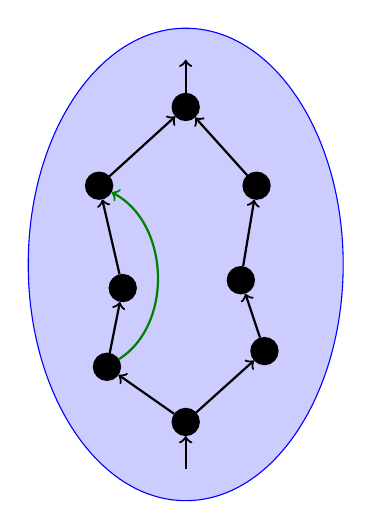
\begin{tikzpicture}[main/.style = {draw, circle, thick, fill}]
			% Draw ellipsoid
			\draw[blue, fill=blue!20] (0,0) ellipse (2 and 3);
			\node[main] (1) at (0,-2) {};
			\node[main] (2) at (-1,-1.3) {};
			\node[main] (3) at (1,-1.1) {};
			\node[main] (4) at (-0.8,-0.3) {};
			\node[main] (5) at (0.7,-0.2) {};
			\node[main] (6) at (-1.1,1) {};
			\node[main] (7) at (0.9,1) {};
			\node[main] (8) at (0,2) {};
			
			\draw[->, thick] (1) edge (2);
			\draw[->, thick] (1) edge (3);
			\draw[->, thick] (2) edge (4);
			\draw[->, thick] (3) edge (5);
			\draw[->, thick] (4) edge (6);
			\draw[->, thick] (5) edge (7);
			\draw[->, thick] (6) edge (8);
			\draw[->, thick] (7) edge (8);
			
			\draw[->, thick] (0, -2.6) -- (1);
			\draw[->, thick] (8) -- (0, 2.6);
			
			\draw[->, thick, color=Green, bend right = 60] (2) edge (6);
		\end{tikzpicture}
	\end{subfigure}
	\begin{subfigure}{0.45\textwidth}\centering
		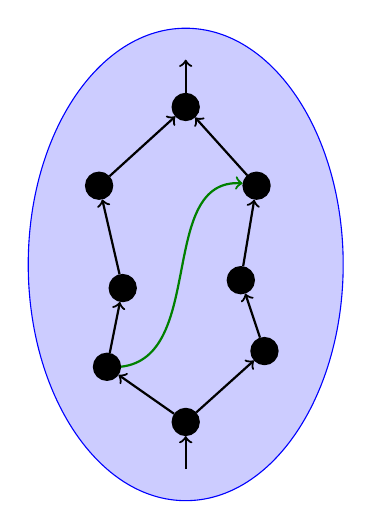
\begin{tikzpicture}[main/.style = {draw, circle, thick, fill}]
			% Draw ellipsoid
			\draw[blue, fill=blue!20] (0,0) ellipse (2 and 3);
			\node[main] (1) at (0,-2) {};
			\node[main] (2) at (-1,-1.3) {};
			\node[main] (3) at (1,-1.1) {};
			\node[main] (4) at (-0.8,-0.3) {};
			\node[main] (5) at (0.7,-0.2) {};
			\node[main] (6) at (-1.1,1) {};
			\node[main] (7) at (0.9,1) {};
			\node[main] (8) at (0,2) {};
			
			\draw[->, thick] (1) edge (2);
			\draw[->, thick] (1) edge (3);
			\draw[->, thick] (2) edge (4);
			\draw[->, thick] (3) edge (5);
			\draw[->, thick] (4) edge (6);
			\draw[->, thick] (5) edge (7);
			\draw[->, thick] (6) edge (8);
			\draw[->, thick] (7) edge (8);
			
			\draw[->, thick] (0, -2.6) -- (1);
			\draw[->, thick] (8) -- (0, 2.6);
			
			\draw[->, thick, color=Green, bend right, out=-50, in=120] (2) edge (7);
		\end{tikzpicture}
	\end{subfigure}
	\caption{An illustration to adding an ear in the construction of an $s-t$ numbering and a corresponding upward drawing.}
\end{figure}

\section{Rectangle visibility representations}

\begin{defn}
	A \textbf{rectangle visibility representation} of a plane graph $G$ is an arrangement of disjoint axes-aligned rectangles in the plane such that the (unions of) horizontal sides of the rectangles correspond to the vertices of $G$, the (unions of) vertical sides to the faces of $G$, and each rectangle corresponds to the edge joining the vertices containing the upper and lower sides of the rectangle, and at the same time to the dual edge joining the faces corresponding to the left and right sides of the rectangle.
\end{defn}

\begin{comm}
	In this section we allow multiple edges without explicitly talking about \\ multigraphs. Moreover, we artificially choose two vertices on the boundary of the outerface and divide the outerface into two faces by "infinite" dummy edges starting in these points.
\end{comm}

\begin{figure}[!ht]\centering
	\begin{subfigure}{0.6\textwidth}\centering
		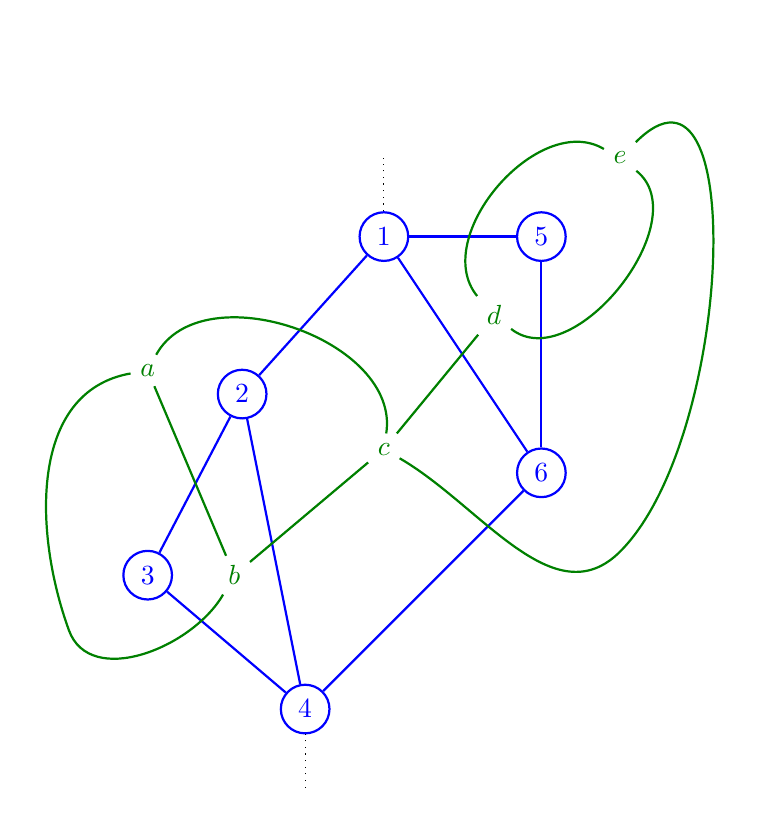
\begin{tikzpicture}[main/.style = {draw, circle, thick, color = Blue}]
			\node[main] (4) at (0,0) {4};
			\node[main] (3) at (-2,1.7) {3};
			\node[main] (6) at (3,3) {6};
			\node[main] (2) at (-0.8,4) {2};
			\node[main] (5) at (3,6) {5};
			\node[main] (1) at (1,6) {1};
			\node[color=Green] (b) at (-0.9, 1.7) {$b$};
			\node[color=Green] (a) at (-2, 4.3) {$a$};
			\node[color=Green] (c) at (1, 3.3) {$c$};
			\node[color=Green] (d) at (2.4, 5) {$d$};
			\node[color=Green] (e) at (4, 7) {$e$};
			\draw[thick, color=Blue] (4) edge (3);
			\draw[thick, color=Blue] (4) edge (2);
			\draw[thick, color=Blue] (4) edge (6);
			\draw[thick, color=Blue] (5) edge (6);
			\draw[thick, color=Blue] (6) edge (1);
			\draw[thick, color=Blue] (2) edge (1);
			\draw[thick, color=Blue] (1) edge (5);
			\draw[thick, color=Blue] (2) edge (3);
			\draw[dotted] (0, -1) -- (4);
			\draw[dotted] (1) -- (1, 7);
			\draw[thick, color=Green] (b) edge (c);
			\draw[thick, color=Green] (d) edge (c);
			\draw[thick, color=Green] (b) edge (a);
			
			\coordinate (6') at (4,2);
			\coordinate (3') at (-3, 1);
			
			\draw[thick, color=Green] (b) to[out = 240, in = -70] (3') to[out = 110, in = 190] (a);
			\draw[thick, color=Green, bend left = 80] (a) edge (c);
			\draw[thick, color=Green] (e) to[out = 45, in = 45] (6') to[out = -135, in = -30] (c);
			\draw[thick, color=Green, bend left = 80] (d) edge (e);
			\draw[thick, color=Green, bend right = 90] (d) edge (e);
		\end{tikzpicture}
	\end{subfigure}
	\begin{subfigure}{0.35\textwidth}\centering
		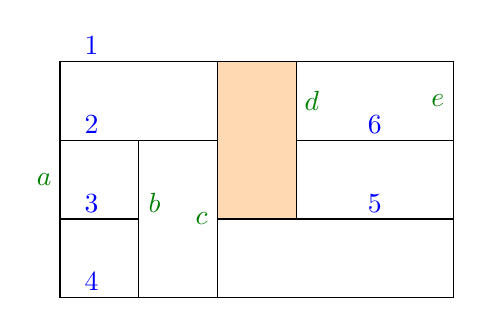
\begin{tikzpicture}
			\draw[black] (0,0) rectangle (1,1);
			\draw[black] (0,1) rectangle (1,2);
			\draw[black] (1,0) rectangle (2,2);
			\draw[black] (2,0) rectangle (5,1);
			\draw[black] (0,2) rectangle (2,3);
			\draw[black, fill=orange!30] (2,1) rectangle (3,3);
			\draw[black] (3,1) rectangle (5,2);
			\draw[black] (3,2) rectangle (5,3);
			\node[Blue] at (0.4, 3.2) {1};
			\node[Blue] at (0.4, 2.2) {2};
			\node[Blue] at (0.4, 1.2) {3};
			\node[Blue] at (0.4, 0.2) {4};
			\node[Green] at (-0.2, 1.5) {$a$};
			\node[Green] at (1.2, 1.2) {$b$};
			\node[Green] at (1.8, 1) {$c$};
			\node[Blue] at (4, 1.2) {5};
			\node[Blue] at (4, 2.2) {6};
			\node[Green] at (3.2, 2.5) {$d$};
			\node[Green] at (4.8, 2.5) {$e$};
		\end{tikzpicture}
	\end{subfigure}
	\caption{An example of a rectangle visibility representation of a planar graph. The highlighted rectangle in the representation corresponds to the primal edge 13 and dual edge $cd$.}
\end{figure}

\begin{thm}
	Every planar vertex 2-connected graph has a rectangle visibility \\ representation.
	\label{thm-2}
\end{thm}

\begin{proof}
	We in fact describe an algorithm how such a representation can be constructed. The bonus is that the construction runs in polynomial time.
\end{proof}

\begin{algorithm}[!ht]
	\caption{RectangleVisibilityRep}
	\begin{algorithmic}[1]
		\Require A planar graph $G$.
		\State Construct an $s - t$ numbering and a corresponding upward planar drawing as in Theorem \ref{thm-1}.
		\State Number the vertices as $1, \dots, n$ according to their $y$-coordinates (1 is the lowest vertex, $n$ is the highest one).
		\State Add a dummy arc from 1 to $n$ drawn to the right of the drawing of $G$, denote by $G'$ the resulting graph.
		\State Construct the dual graph $G^\ast$ to $G'$, and orient its edges so that each edge of $G$ is crossed by its dual edge from left to right, while the added dummy edge is crossed from right to left. Let $n^\ast$ be the number of vertices of $G^\ast$.
		\State Consider a topological sorting of the vertices of $G^\ast$ and name them $A, B, \dots$ according to this sorting.
		\State Take a grid of size $n \times n^\ast$. For a vertex $i$ of $G$, let $\alpha(\beta)$ be the face incident with $i$ with the lowest (highest, respectively) name in the topological sorting of $G^\ast$. Represent $i$ by a horizontal segment on the $i$-th line, starting at the vertical line $\alpha$ and ending on the vertical line $\beta$. For a face $\alpha$ of the drawing of $G'$ (i.e., a vertex of the dual graph $G^\ast$), let $i$ be its lowest vertex and $j$ its highest vertex (with respect to the topological sorting of $G$). Represent $\alpha$ by a segment on the vertical line $\alpha$, starting on the $i$-th horizontal line and ending on the $j$-th one.
		\State \Return this representation.
	\end{algorithmic}
\end{algorithm}

It is, however, necessary to prove that this Algorithm really outputs a rectangle visibility representation of $G$. This is done via a series of claims. The first ones talk about the upward drawing of $G$ constructed in Step 1 and the dual graph $G^\ast$ and its drawing inherited from the drawing of $G$.

\begin{claim}
	Vertex number 1 and vertex number $n$ are both on the boundary of the outerface of $G$ (and also of $G'$). The face that gets the name $A$ is the unbounded face and the face with the highest name, say $Z$, is the other face incident with the dummy edge $1n$.
\end{claim}

\begin{claim}
	The orientation of $G^\ast$ described in Step 4 is acyclic and $A$ is its only source and $Z$ is its only sink. Hence it is indeed an $s - t$ numbering of $G^\ast$. To see this, note first that the edge $AZ$ which crosses the dummy edge $1n$ cannot be involved in any directed cycle, as $A$ is a source and $Z$ is a sink in $G^\ast$. Next observe that a clock-wise oriented cycle in $G^\ast$ would bound a region with at least one vertex of $G$ inside and all edges of $G$ crossing this cycle would be oriented from inside towards the outside of this region, hence, there would necessarily be a source of $G$ in this region, and this would be different from the vertex $1$. Similarly, a counter-clock-wise oriented cycle in $G^\ast$ would bound a region that would contain a sink different from $n$. This would be a contradiction with the assumption that we were working with an $s - t$-numbering of $G$. Finally, a source different from $A$ (a sink different from $Z$) in $G^\ast$ would yield a directed cycle on the boundary of this face of $G$. A contradiction again.
\end{claim}

\begin{claim}
	The boundary of every face $\alpha$ of $G$ consists of two directed paths, the left one and the right one, both connecting the vertex of the lowest number to the vertex of the highest number among the vertices of this face. We have seen this in the proof of Theorem \ref{thm-1}.
\end{claim}

\begin{claim}
	For every vertex $i$ of $G, i \neq 1, n$, the faces incident with $i$ induce two directed paths in $G^\ast$,
	both connecting the face to the left of $i$ to the face lying to the right of $i$, one of the paths passing
	through the faces for which $i$ is their topmost vertex, the other one passing through the faces for which
	$i$ is their lowest vertex. See Fig. \ref{fig-3} right.
	\label{claim-4}
\end{claim}

\begin{figure}[!ht]
	\begin{subfigure}{0.45\textwidth}\centering
		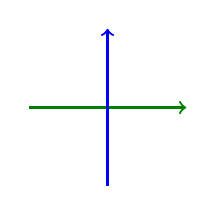
\begin{tikzpicture}
			\draw[->, color=Green, thick] (0,0) -- (2,0);
			\draw[->, color=Blue, thick] (1, -1) -- (1, 1);
		\end{tikzpicture}
		\caption{Orientation of the dual edges.}
	\end{subfigure}
	\begin{subfigure}{0.45\textwidth}\centering
		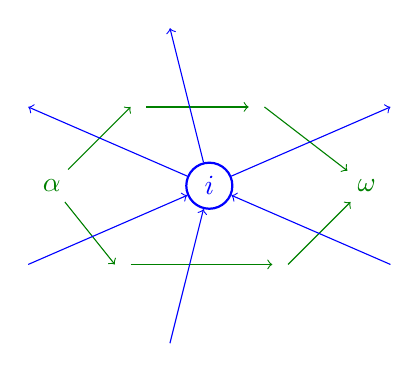
\begin{tikzpicture}
			\node[draw, circle, Blue, thick] (i) at (0,0) {$i$};
			\node[Green, thick] (a) at (-2, 0) {$\alpha$};
			\node[Green, thick] (w) at (2,0) {$\omega$};
			\draw[->, Green] (a) -- (-1, 1);
			\draw[->, Green] (-0.8,1) -- (0.5, 1);
			\draw[->, Green] (0.7, 1) -- (w);
			\draw[->, Green] (a) -- (-1.2, -1);
			\draw[->, Green] (-1, -1) -- (0.8, -1);
			\draw[->, Green] (1, -1) -- (w);
			\draw[->, Blue] (i) -- (-0.5, 2);
			\draw[->, Blue] (-0.5, -2) -- (i);
			\draw[->, Blue] (i) -- (-2.3, 1);
			\draw[->, Blue] (-2.3, -1) -- (i);
			\draw[->, Blue] (i) -- (2.3, 1);
			\draw[->, Blue] (2.3, -1) -- (i);
		\end{tikzpicture}
		\caption{An example to the statement of Claim \ref{claim-4}.}
	\end{subfigure}
	\caption{Examples for claims.}
	\label{fig-3}
\end{figure}

In the next claims we prove that the collection of segments constructed in Step 6 defines a rectangle visibility representation of $G$.

\begin{claim}
	Let $i$ be a vertex of $G, i \neq 1, n$. Let $\alpha$ and $\omega$ be the faces to the left and to the right of $i$, respectively. Then the (horizontal) segment $i$ touches the vertical segment for $\alpha$ from the right, it touches the vertical segment for $\beta$ from the left, it is touched by the segments representing the faces lying on the upper path from $\alpha$ to $\beta$ in $G^\ast$ from above, and it is touched by the faces lying on the lower path from $\alpha$ to $\beta$ in $G^\ast$ from below. The segment representing vertex $1$ spans the whole range from $A$ to $Z$ and is only touched by vertical segments from above, while the segment representing $n$ is only touched by vertical segments from below, and also spans the whole range from $A$ to $Z$.
	\label{claim-5}
\end{claim}

\begin{claim}
	Let $\alpha$ be an inner face of $G$, i.e., a face not incident with the dummy edge $1n$. The vertical segment representing $\alpha$ touches the horizontal segment representing its lowest vertex from above, it touches the segment representing its topmost vertex from below, it is touched by the segments representing the vertices on the left boundary path of $\alpha$ from the left and it is touched by the segments representing the vertices on the right boundary path of $\alpha$ from the right. The segment representing $A$ is touched only from right, while the segment representing $Z$ is touched only from left, always by the appropriate horizontal segments.
	\label{claim-6}
\end{claim}

\begin{figure}[!ht]
	\begin{subfigure}{.25\textwidth}\centering
		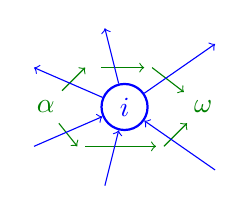
\begin{tikzpicture}
			\node[draw, circle, Blue, thick] (i) at (0,0) {$i$};
			\node[Green, thick] (a) at (-1, 0) {$\alpha$};
			\node[Green, thick] (w) at (1,0) {$\omega$};
			\draw[->, Green] (a) -- (-0.5, 0.5);
			\draw[->, Green] (-0.3,0.5) -- (0.25, 0.5);
			\draw[->, Green] (0.35, .5) -- (w);
			\draw[->, Green] (a) -- (-.6, -.5);
			\draw[->, Green] (-.5, -.5) -- (0.4, -.5);
			\draw[->, Green] (.5, -.5) -- (w);
			\draw[->, Blue] (i) -- (-0.25, 1);
			\draw[->, Blue] (-0.25, -1) -- (i);
			\draw[->, Blue] (i) -- (-1.15, .5);
			\draw[->, Blue] (-1.15, -.5) -- (i);
			\draw[->, Blue] (i) -- (1.15, .8);
			\draw[->, Blue] (1.15, -.8) -- (i);
		\end{tikzpicture}
	\end{subfigure}
	\begin{subfigure}{.2\textwidth}\centering
		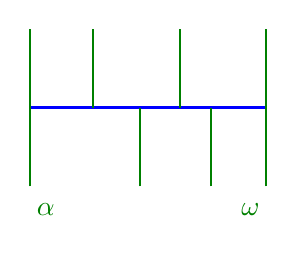
\begin{tikzpicture}
			\draw[thick, Blue] (0,0) -- (3,0);
			\draw[thick, Green] (0,-1) -- (0,1);
			\draw[thick, Green] (3,-1) -- (3,1);
			\draw[thick, Green] (.8,0) -- (.8,1);
			\draw[thick, Green] (1.9,0) -- (1.9,1);
			\draw[thick, Green] (1.4,-1) -- (1.4,0);
			\draw[thick, Green] (2.3,-1) -- (2.3,0);
			\node[Green] at (.2, -1.3) {$\alpha$};
			\node[Green] at (2.8, -1.3) {$\omega$};
		\end{tikzpicture}
	\end{subfigure}
	\begin{subfigure}{.25\textwidth}\centering
		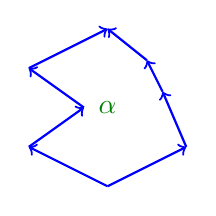
\begin{tikzpicture}
			\draw[->, thick, Blue] (0,0) -- (-1, .5);
			\draw[->, thick, Blue] (-1, .5) -- (-.3, 1);
			\draw[->, thick, Blue] (-.3, 1) -- (-1, 1.5);
			\draw[->, thick, Blue] (-1, 1.5) -- (0, 2);
			\draw[->, thick, Blue] (0,0) -- (1, .5);
			\draw[->, thick, Blue] (1, .5) -- (.7, 1.2);
			\draw[->, thick, Blue] (.7, 1.2) -- (.5, 1.6);
			\draw[->, thick, Blue] (.5, 1.6) -- (0,2);
			\node[Green, thick] at (0,1) {$\alpha$};
		\end{tikzpicture}
	\end{subfigure}
	\begin{subfigure}{.2\textwidth}\centering
		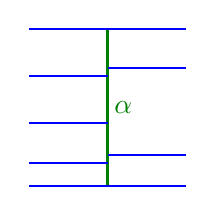
\begin{tikzpicture}
			\draw[Green, thick] (0,0) -- (0,2);
			\draw[Blue, thick] (-1,0) -- (1,0);
			\draw[Blue, thick] (-1,2) -- (1,2);
			\draw[Blue, thick] (-1,.3) -- (0,.3);
			\draw[Blue, thick] (-1,.8) -- (0,.8);
			\draw[Blue, thick] (-1,1.4) -- (0,1.4);
			\draw[Blue, thick] (0,.4) -- (1,.4);
			\draw[Blue, thick] (0,1.5) -- (1,1.5);
			\node[Green, thick] at (0.2, 1) {$\alpha$};
		\end{tikzpicture}
	\end{subfigure}
	\caption{Illustration to Claims \ref{claim-5} and \ref{claim-6}.}
\end{figure}

\begin{claim}
	For every edge $ij$ of $G$, let $\alpha\beta$ be its dual edge. Then the segments representing $i, j, \alpha$ and $\beta$ bound a rectangle in the representation.
	\label{claim-7}
\end{claim}

\begin{claim}
	No two segments constructed in Step 6 cross each other. For suppose segment $j$ crosses segment $\alpha$. By the way the segments are constructed, this means that there exist vertices $i, k, i < j < k$, and $\beta, \gamma, \beta < \alpha < \gamma$, such that $i$ is the lowest and $k$ the topmost vertex of face $\alpha$ and $\beta$ is the left and $\gamma$ the right face incident with $j$. Consider the upward drawing of $G$ and the horizontal stripe of vertices with their $y$-coordinates between $i$ and $k$. The face $\alpha$ spans this stripe from its bottom to its top lines, and thus it lies either to the left or to the right of vertex $i$. Suppose it is to the left. The horizontal ray starting in vertex $i$ and pointing to the left passes first through the face $\beta$ and then crosses several faces until it finally crosses $\alpha$. Since all edges of $G$ it crosses on this way are directed upward, these faces form a path directed from $\alpha$ to $\beta$ in $G^\ast$, which means that $\alpha < \beta$ in the topological sorting of $G^\ast$. Which is a contradiction.
	\label{claim-8}
\end{claim}

\begin{figure}
	\begin{subfigure}{.45\textwidth}\centering
		\begin{tikzpicture}
			\draw[thick, Green] (0,0) -- (0,3);
			\draw[thick, Blue] (-1.5,1.5) -- (1.5, 1.5);
			\draw[dotted] (-1.5, -.2) -- (-1.5, 3.2);
			\draw[dotted] (1.5, -.2) -- (1.5, 3.2);
			\draw[dotted] (-1.7, 0) -- (1.7, 0);
			\draw[dotted] (-1.7, 3) -- (1.7, 3);
			
			\node[Green] at (.3, .2) {$\alpha$};
			\node[Blue] at (1.2, 1.8) {$j$};
			\node[Blue] at (1.9, 0) {$i$};
			\node[Blue] at (1.9, 3) {$k$};
			\node[Green] at (-1.2, -.3) {$\beta$};
			\node[Green] at (1.2, -.3) {$\gamma$};
		\end{tikzpicture}
	\end{subfigure}
	\begin{subfigure}{.45\textwidth}\centering
		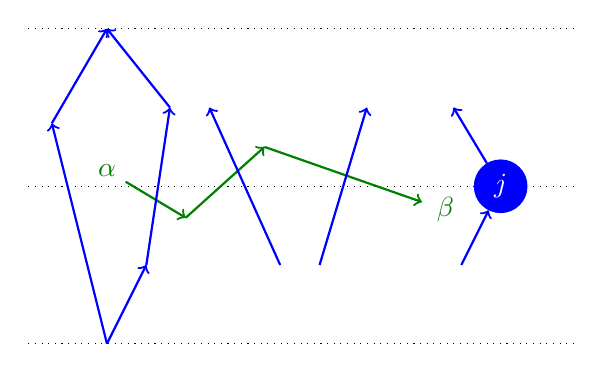
\begin{tikzpicture}
			\draw[dotted] (0,0) -- (7,0);
			\draw[dotted] (0,2) -- (7,2);
			\draw[dotted] (0,-2) -- (7,-2);
			\node[Green] (a) at (1, 0.2) {$\alpha$};
			\draw[->, thick, Green] (a) -- (2, -.4);
			\draw[->, thick, Green] (2, -.4) -- (3, .5);
			\draw[->, thick, Green] (3, .5) -- (5, -.2);
			\node[Green] (b) at (5.3, -.3) {$\beta$};
			\node[draw, circle, Blue, fill] (j) at (6, 0) {\textcolor{white}{$j$}};
			\draw[->, Blue, thick] (5.5, -1) -- (j);
			\draw[->, Blue, thick] (j) -- (5.4, 1);
			\draw[->, thick, Blue] (3.7, -1) -- (4.3,1);
			\draw[->, thick, Blue] (3.2, -1) -- (2.3,1);
			\draw[->, thick, Blue] (1.5, -1) -- (1.8,1);
			\draw[->, thick, Blue] (1,-2) -- (1.5, -1);
			\draw[->, thick, Blue] (1.8, 1) -- (1,2);
			\draw[->, thick, Blue] (1,-2) -- (.3, .8);
			\draw[->, thick, Blue] (.3, .8) -- (1,2);
		\end{tikzpicture}
	\end{subfigure}
	\caption{An illustration to Claim \ref{claim-8}.}
\end{figure}

\begin{claim}
	The rectangles from Claim \ref{claim-7} are disjoint and fill in the base rectangle formed by segments $A, Z, 1, n$. This now follows from the previous claims. And this means that we have indeed constructed a rectangle visibility representation of $G$.
\end{claim}

\begin{figure}[!ht]
	\begin{subfigure}{0.53\textwidth}\centering
		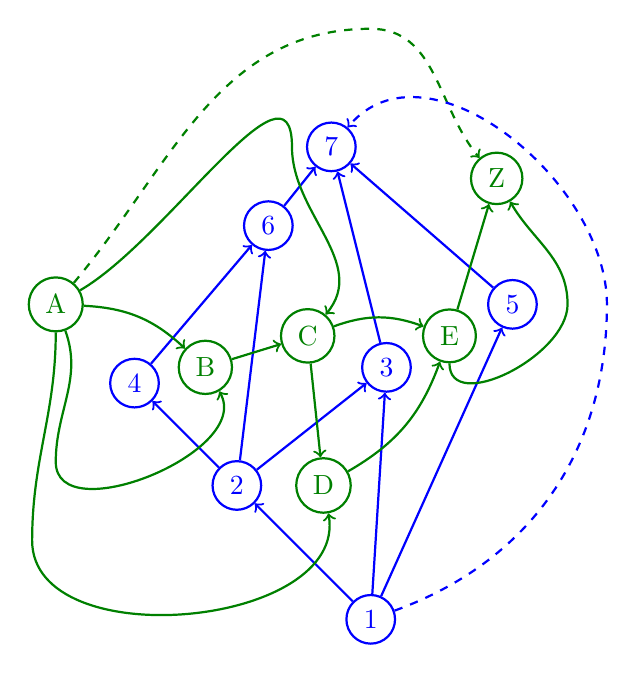
\begin{tikzpicture}[be/.style = {thick, Blue, ->}, ge/.style = {thick, Green, ->},
			bn/.style = {Blue, thick, circle, draw}, gn/.style = {Green, thick, circle, draw}]
			\node[bn] (1) at (0,0) {1};
			\node[bn] (2) at (-1.7, 1.7) {2};
			\node[bn] (3) at (.2, 3.2) {3};
			\node[bn] (4) at (-3, 3) {4};
			\node[bn] (5) at (1.8, 4) {5};
			\node[bn] (6) at (-1.3, 5) {6};
			\node[bn] (7) at (-.5, 6) {7};
			\node[gn] (A) at (-4, 4) {A};
			\node[gn] (B) at (-2.1, 3.2) {B};
			\node[gn] (C) at (-.8, 3.6) {C};
			\node[gn] (D) at (-.6, 1.7) {D};
			\node[gn] (E) at (1, 3.6) {E};
			\node[gn] (Z) at (1.6, 5.6) {Z};
			\draw[be] (1) -- (2);
			\draw[be] (1) -- (3);
			\draw[be] (1) -- (5);
			\draw[be] (2) -- (4);
			\draw[be] (2) -- (6);
			\draw[be] (2) -- (3);
			\draw[be] (5) -- (7);
			\draw[be] (3) -- (7);
			\draw[be] (6) -- (7);
			\draw[be] (4) -- (6);
			\draw[ge, bend left = 20] (A) edge (B);
			\draw[ge] (B) -- (C);
			\draw[ge] (C) -- (D);
			\draw[ge] (E) -- (Z);
			\draw[ge, bend right = 20] (D) edge (E);
			\draw[ge, bend left = 20] (C) edge (E);
			\draw[ge] (A) to[out=290, in=90] (-4, 2) to[out=270, in=300] (B);
			\draw[ge] (A) to[out=270, in=90] (-4.3, 1) to[out=270, in=280] (D);
			\draw[ge] (A) to[out=30, in=90] (-1, 6) to[out=270, in=50] (C);
			\draw[ge] (E) to[out=270, in=270] (2.5, 4) to[out=90, in=300] (Z);
			\draw[ge, dashed] (A) to[out=50, in=180] (0, 7.5) to[out=0, in=130] (Z);
			\draw[be, dashed] (1) to[out=20, in=270] (3, 4) to[out=90, in=50] (7);
		\end{tikzpicture}
	\end{subfigure}
	\begin{subfigure}{0.45\textwidth}\centering
		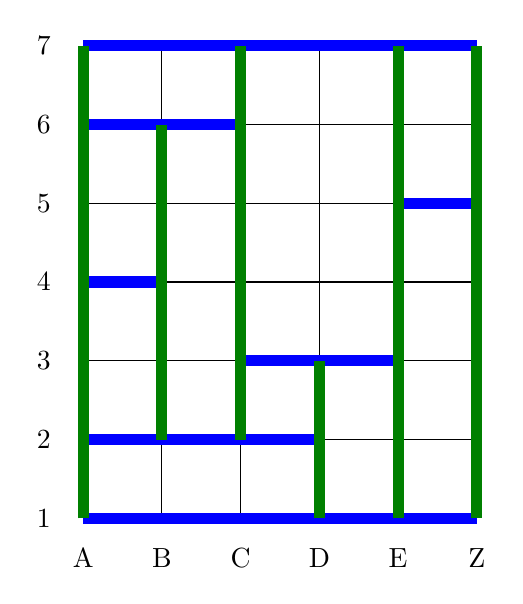
\begin{tikzpicture}[b/.style = {line width = 4, Blue}, g/.style = {line width = 4, Green}]
			\draw (1,1) -- (1,7);
			\draw (2,1) -- (2,7);
			\draw (3,1) -- (3,7);
			\draw (4,1) -- (4,7);
			\draw (5,1) -- (5,7);
			\draw (6,1) -- (6,7);
			\draw (1,1) -- (6,1);
			\draw (1,2) -- (6,2);
			\draw (1,3) -- (6,3);
			\draw (1,4) -- (6,4);
			\draw (1,5) -- (6,5);
			\draw (1,6) -- (6,6);
			\draw (1,7) -- (6,7);
			\draw[b] (1,1) -- (6,1);
			\draw[b] (1,2) -- (4,2);
			\draw[b] (3,3) -- (5,3);
			\draw[b] (1,4) -- (2,4);
			\draw[b] (5,5) -- (6,5);
			\draw[b] (1,6) -- (3,6);
			\draw[b] (1,7) -- (6,7);
			\draw[g] (1,1) -- (1,7);
			\draw[g] (2,2) -- (2,6);
			\draw[g] (3,2) -- (3,7);
			\draw[g] (4,1) -- (4,3);
			\draw[g] (5,1) -- (5,7);
			\draw[g] (6,1) -- (6,7);
			\node at (.5, 1) {1};
			\node at (.5, 2) {2};
			\node at (.5, 3) {3};
			\node at (.5, 4) {4};
			\node at (.5, 5) {5};
			\node at (.5, 6) {6};
			\node at (.5, 7) {7};
			\node at (1,.5) {A};
			\node at (2,.5) {B};
			\node at (3,.5) {C};
			\node at (4,.5) {D};
			\node at (5,.5) {E};
			\node at (6,.5) {Z};
		\end{tikzpicture}
	\end{subfigure}
	\caption{An overview of the construction by Algorithm RectangleVisibilityRep.}
\end{figure}

\section{Grid Contact graphs}

\begin{defn}
	A graph is a \textbf{Grid Intersection graph} if it has an intersection \\ representation by vertical and horizontal segments in which no two segments of the same direction share a point (in other words, all vertical, as well as all horizontal, segments are pairwise disjoint). A graph is a \textbf{Grid Contact} graph if it has a Grid Intersection representation in which no two segments cross, i.e., any two non-disjoint segments only touch each other.
\end{defn}

\begin{prop}
	Every grid intersection graph is bipartite. Moreover, every grid contact graph is planar.
\end{prop}

\begin{proof}
	The first claim is a simple observation. For the second claim, note that grid contact graphs form a subclass of triangle-free contact graphs of arc-connected regions in the plane. All such graphs are planar, since a non-crossing drawing can be constructed from a contact representation by selecting a point inside each region to represent its vertex, and connecting it to the contact points with the adjacent regions by curves inside the region.
\end{proof}

\begin{thm}
	Every planar bipartite graph is a grid contact graph.
	\label{thm-3}
\end{thm}

\begin{proof}
	Given a planar bipartite graph $G = (A \cup B, E)$, consider a non-crossing drawing and extend it to a non-crossing drawing of a supergraph $G' = (A' \cup B' , E')$ such that
	
	\begin{itemize}
		\item $G$ is an induced subgraph of $G'$,
		\item every face of the drawing of $G'$ is bounded by a cycle of length 4 (i.e., $G'$ is a so called quadrangulation),
		\item every vertex of $G'$ has degree greater than $2$, and
		\item no vertex of $B$ is on the boundary of the outerface of $G'$. 
	\end{itemize}
	
	Then construct the graph $\bar{G} = (A', \bar{E})$ by putting $\bar{E}$ the diagonals of the faces of $G'$ connecting their $A'$-vertices. It can be easily seen that $G$ is vertex 2-connected and that the faces of $\bar{G}$ are in 1-1 correspondence with the vertices of $B'$. Thus the segments of a rectangle visibility representation of $\bar{G}$ constructed as in the proof of Theorem \ref{thm-2} form a grid contact representation of $G'$ . Note the technical detail that the vertex (of $B'$) that corresponds to the outerface of $\bar{G}$ is represented by two vertical segments, not one. But this vertex does not belong to $B$, and so the segments corresponding to the vertices of $G$ form a grid contact representation of $G$.
\end{proof}

\begin{figure}[!ht]
	\begin{subfigure}{0.45\textwidth}\centering
		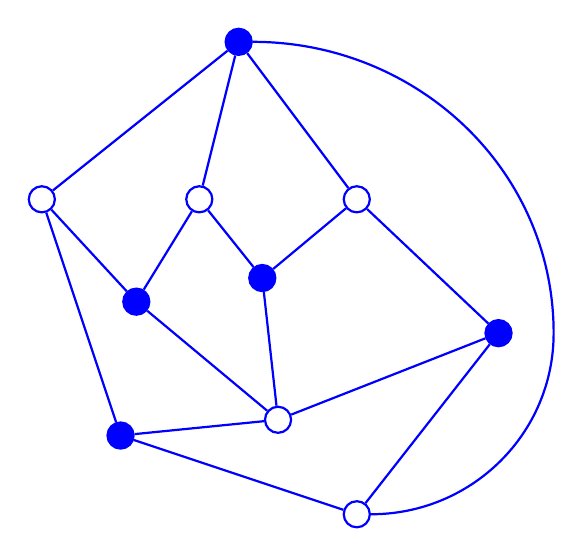
\begin{tikzpicture}[main/.style = {draw, circle, thick, Blue},
			edge/.style = {thick, Blue},
			fil/.style = {thick, fill, draw, circle, Blue}]
			\node[main] (1) at (0,0) {};
			\node[fil] (2) at (1.8, 2.3) {};
			\node[fil] (3) at (-3, 1) {};
			\node[main] (4) at (-1, 1.2) {};
			\node[fil] (5) at (-1.2, 3) {};
			\node[fil] (6) at (-2.8, 2.7) {};
			\node[main] (7) at (-4, 4) {};
			\node[main] (8) at (-2, 4) {};
			\node[main] (9) at (0, 4) {};
			\node[fil] (10) at (-1.5, 6) {};
			\draw[edge] (1) -- (2);
			\draw[edge] (1) -- (3);
			\draw[edge] (3) -- (4);
			\draw[edge] (2) -- (4);
			\draw[edge] (4) -- (5);
			\draw[edge] (4) -- (6);
			\draw[edge] (2) -- (9);
			\draw[edge] (9) -- (10);
			\draw[edge] (8) -- (10);
			\draw[edge] (7) -- (10);
			\draw[edge] (3) -- (7);
			\draw[edge] (6) -- (7);
			\draw[edge] (5) -- (8);
			\draw[edge] (6) -- (8);
			\draw[edge] (5) -- (9);
			\draw[edge] (1) to[out=0, in=270] (2.5, 2.3) to[out=90, in=0] (10);
		\end{tikzpicture}
		\caption{The graph $G'$.}
	\end{subfigure}
	\begin{subfigure}{0.53\textwidth}\centering
		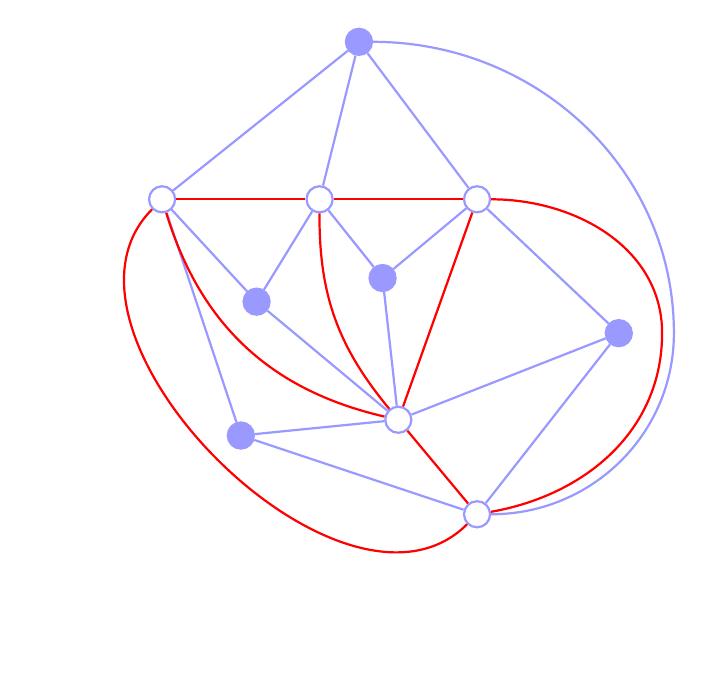
\begin{tikzpicture}[main/.style = {draw, circle, thick, Blue!40},
			edge/.style = {thick, Blue!40},
			fil/.style = {thick, fill, draw, circle, Blue!40},
			red/.style = {thick, Red}]
			\node[main] (1) at (0,0) {};
			\node[fil] (2) at (1.8, 2.3) {};
			\node[fil] (3) at (-3, 1) {};
			\node[main] (4) at (-1, 1.2) {};
			\node[fil] (5) at (-1.2, 3) {};
			\node[fil] (6) at (-2.8, 2.7) {};
			\node[main] (7) at (-4, 4) {};
			\node[main] (8) at (-2, 4) {};
			\node[main] (9) at (0, 4) {};
			\node[fil] (10) at (-1.5, 6) {};
			\draw[edge] (1) -- (2);
			\draw[edge] (1) -- (3);
			\draw[edge] (3) -- (4);
			\draw[edge] (2) -- (4);
			\draw[edge] (4) -- (5);
			\draw[edge] (4) -- (6);
			\draw[edge] (2) -- (9);
			\draw[edge] (9) -- (10);
			\draw[edge] (8) -- (10);
			\draw[edge] (7) -- (10);
			\draw[edge] (3) -- (7);
			\draw[edge] (6) -- (7);
			\draw[edge] (5) -- (8);
			\draw[edge] (6) -- (8);
			\draw[edge] (5) -- (9);
			\draw[edge] (1) to[out=0, in=270] (2.5, 2.3) to[out=90, in=0] (10);
			\draw[red] (1) edge (4);
			\draw[red, bend right = 30] (7) edge (4);
			\draw[red, bend left = 90] (1) edge (7);
			\draw[red, bend right = 20] (8) edge (4);
			\draw[red] (4) edge (9);
			\draw[red] (8) edge (9);
			\draw[red] (1) to[out=10, in=270] (2.35, 2.3) to[out=90, in=0] (9);
			\draw[red] (7) edge (8);
		\end{tikzpicture}
		\caption{The graph $G$.}
	\end{subfigure}
	\caption{An illustration to the proof of Theorem \ref{thm-3}.}
\end{figure}
	\chapter{Schnyder woods}

\section{Canonical ordering}

\begin{defn}
	Given a plane triangulation (i.e., a non-crossing embedding of a trian-\\gulation in the plane, which means that the outerface is fixed) $G = (V, E)$, a canonical ordering of it is a numbering $1, 2, \dots, n$ of its vertices such that
	
	\begin{enumerate}[i)]
		\item the vertices of the outerface are $1, 2$ and $n = |V|$,
		\item for every $i = 3, 4, \dots, n - 1$,
		\begin{enumerate}[a)]
			\item the graph $G_i = G[1, 2, \dots, i]$ is vertex 2-connected,
			\item all vertices $j \leq i$ are drawn inside (or on the boundary) of the embedding of $G_i$ inherited from the embedding of $G$,
			\item all vertices $j > i$ are drawn outside the embedding of $G_i$ inherited from the embedding of $G$,
			\item the neighbors of vertex $i + 1$ in $G_i$ are lying consecutively on the boundary of $G_i$.
		\end{enumerate}
	\end{enumerate}
\end{defn}

\begin{thm}
	Every triangulation has a canonical ordering.
\end{thm}

\begin{proof}
	By induction from $n$ downto $3$, assign the numbers to the vertices. Once $n, n - 1, \dots, i + 1$ are assigned, choose as vertex $i$ such a vertex on the boundary of $G_i$ whose deletion from $G_i$ leaves $G_{i-1}$ vertex 2-connected. The only obstacle to preserving 2-connectedness is if $i$ would be incident to a diagonal edge (an edge with both end-vertices on the boundary of the outerface, but which itself is not a part of the boundary). But there is always a vertex which is not incident with any diagonal (to observe this, consider a vertex which is incident with a shortest possible diagonal, with the length of a diagonal being measured by the number of vertices of the boundary that it cuts off of $G_i$). So assign $i$ to a vertex (there may be more options) which is not incident to any diagonal. Then a), b) and c) are fulfilled for $G_{i-1}$. Note that d) follows from b) and c).
\end{proof}

\section{Schnyder woods}

\begin{algorithm}[!ht]
	\caption{Schnyder}
	\begin{algorithmic}[1]
		\Require A plane triangulation $G = (V, E)$ and a canonical ordering of it.
		\For{$i := 3 \dots n -1$}
			\State set $b(i)$ to be the leftmost neighbor of $i$ on the boundary of $G_{i-1}$, direct the edge $ib(i)$ in this direction and color it blue;
			\State set $g(i)$ to be the rightmost neighbor of $i$ on the boundary of $G_{i-1}$, direct the edge $ig(i)$ in this direction and color it green;
			\State set $r(i)$ to be the neighbor of $i$ with the highest number, direct the edge $ig(i)$ in this direction and color it red
		\EndFor
		\State \Return the orientation of $G$, the coloring of its edges and the mappings $b, g$ and $r$.
	\end{algorithmic}
\end{algorithm}

\begin{figure}[!ht]\centering
	\begin{subfigure}{0.45\textwidth}\centering
		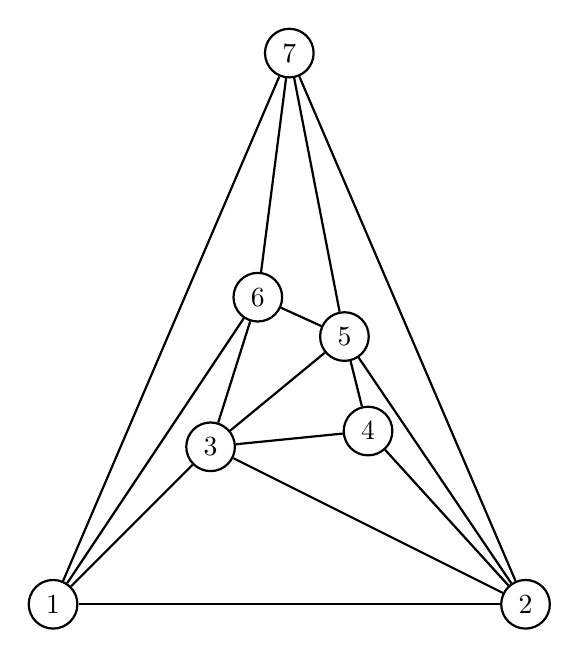
\begin{tikzpicture}[main/.style = {draw, circle, thick}]
			\node[main] (1) at (-1,-1) {1};
			\node[main] (2) at (5,-1) {2};
			\node[main] (3) at (1,1) {3};
			\node[main] (4) at (3, 1.2) {4};
			\node[main] (5) at (2.7, 2.4) {5};
			\node[main] (6) at (1.6, 2.9) {6};
			\node[main] (7) at (2, 6) {7};
			\draw[thick] (1) edge (3);
			\draw[thick] (1) edge (2);
			\draw[thick] (1) edge (7);
			\draw[thick] (1) edge (6);
			\draw[thick] (6) edge (3);
			\draw[thick] (4) edge (3);
			\draw[thick] (5) edge (3);
			\draw[thick] (2) edge (3);
			\draw[thick] (2) edge (4);
			\draw[thick] (2) edge (5);
			\draw[thick] (2) edge (7);
			\draw[thick] (5) edge (4);
			\draw[thick] (5) edge (6);
			\draw[thick] (7) edge (6);
			\draw[thick] (7) edge (5);
		\end{tikzpicture}
	\end{subfigure}
	\begin{subfigure}{0.45\textwidth}\centering
		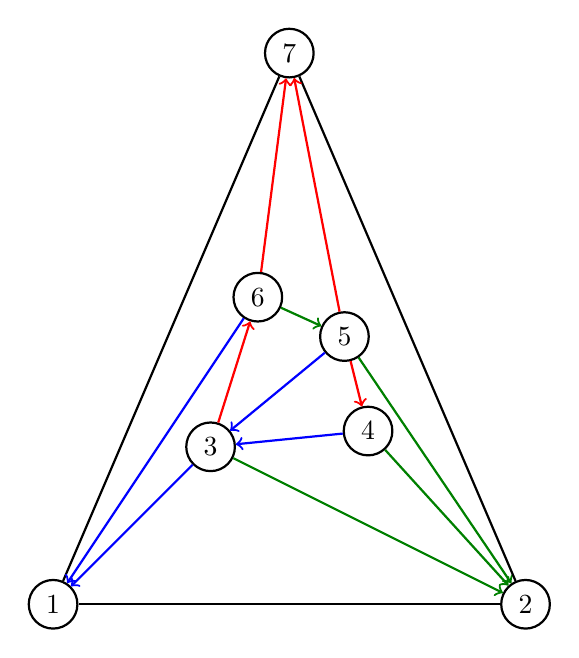
\begin{tikzpicture}[main/.style = {draw, circle, thick}]
			\node[main] (1) at (-1,-1) {1};
			\node[main] (2) at (5,-1) {2};
			\node[main] (3) at (1,1) {3};
			\node[main] (4) at (3, 1.2) {4};
			\node[main] (5) at (2.7, 2.4) {5};
			\node[main] (6) at (1.6, 2.9) {6};
			\node[main] (7) at (2, 6) {7};
			\draw[thick, ->, color=Blue] (3) edge (1);
			\draw[thick] (1) edge (2);
			\draw[thick] (1) edge (7);
			\draw[thick, ->, color=Blue] (6) edge (1);
			\draw[thick, ->, color=Red] (3) edge (6);
			\draw[thick, ->, color=Blue] (4) edge (3);
			\draw[thick, ->, color=Blue] (5) edge (3);
			\draw[thick, ->, color=Green] (3) edge (2);
			\draw[thick, ->, color=Green] (4) edge (2);
			\draw[thick, ->, color=Green] (5) edge (2);
			\draw[thick] (2) edge (7);
			\draw[thick, ->, color=Red] (5) edge (4);
			\draw[thick, ->, color=Green] (6) edge (5);
			\draw[thick, ->, color=Red] (6) edge (7);
			\draw[thick, ->, color=Red] (5) edge (7);
		\end{tikzpicture}
	\end{subfigure}
	\caption{An illustration to canonical orderings and Schnyder woods.}
\end{figure}

\begin{thm}
	The blue edges form a tree rooted in vertex 1 and spanning the vertices $1, 3, \dots, n - 1$, the green edges form a tree rooted in vertex 2 and spanning the vertices $2, 3, \dots, n - 1$, and the red edges form a tree rooted in vertex n and spanning the vertices $3, \dots , n$. Every edge of $G$, except of $12, 1n, 2n$, belongs to exactly one of these trees.
\end{thm}

\begin{proof}
	Clear from the construction and properties of canonical orderings.
\end{proof}

\begin{cor}
	The edges of a planar triangulation can be partitioned into edge sets of 3 trees and a triangle. Such a collection of three trees is called a \textbf{Schnyder wood} of $G$.
\end{cor}

\begin{figure}[!ht]\centering
	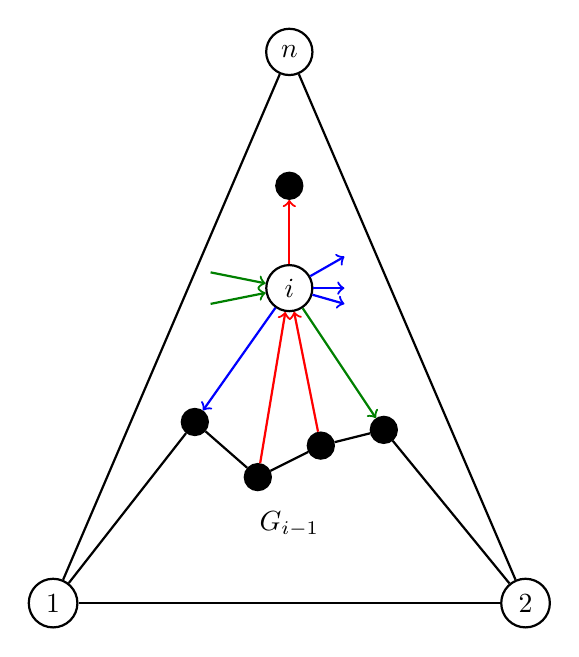
\begin{tikzpicture}[main/.style = {draw, circle, thick}]
		\node[main] (1) at (-1,-1) {1};
		\node[main] (2) at (5,-1) {2};
		\node[main, fill] (3) at (.8,1.3) {};
		\node[main, fill] (4) at (3.2, 1.2) {};
		\node[main, fill] (5) at (2.4, 1) {};
		\node[main, fill] (6) at (1.6, 0.6) {};
		\node[main] (n) at (2, 6) {$n$};
		\node[main] (i) at (2, 3) {$i$};
		\node[main, fill] (7) at (2, 4.3) {};
		\node (G) at (2, 0) {$G_{i-1}$};
		\draw[thick] (1) edge (3);
		\draw[thick] (1) edge (2);
		\draw[thick] (1) edge (n);
		\draw[thick] (6) edge (3);
		\draw[thick] (2) edge (4);
		\draw[thick] (2) edge (n);
		\draw[thick] (5) edge (4);
		\draw[thick] (5) edge (6);		
		\draw[thick, color=Blue, ->] (i) edge (3);
		\draw[thick, color=Red, ->] (6) edge (i);
		\draw[thick, color=Red, ->] (5) edge (i);
		\draw[thick, color=Green, ->] (i) edge (4);
		\draw[thick, color=Red, ->] (i) edge (7);
		\draw[thick, color=Green, ->] (1, 3.2) -- (i);
		\draw[thick, color=Green, ->] (1, 2.8) -- (i);
		\draw[thick, color=Blue, ->] (i) -- (2.7, 3.4);
		\draw[thick, color=Blue, ->] (i) -- (2.7, 2.8);
		\draw[thick, color=Blue, ->] (i) -- (2.7, 3);
	\end{tikzpicture}
	\caption{The rotation scheme of incoming and outgoing edges around a vertex in the Schnyder wood.}
\end{figure}

\begin{prop}
	Locally around every inner vertex of $G$, we see (in the counter-clock-wise order) one outgoing blue edge, several (or none) incoming red edges, one outgoing green edge, several (or none) incoming blue edges, one outgoing red edge, and several (or none) incoming green edges.
\end{prop}

\section{Triangle contact representations}

\begin{thm}[de Fraysseix, Ossona de Mendez, Rosenstiehl]
	Every planar graph is a contact graph of isosceles triangles with horizontal bases.
\end{thm}

\begin{proof}
	It suffices to prove the theorem for triangulations, since every planar graph is an induced subgraph of a triangulation. Given a triangulation $G = (V, E)$, fix an embedding and consider a canonical ordering with respect to this embedding, and run algorithm Schnyder on this canonical ordering. Draw $n + 1 = |V| + 1$ parallel horizontal lines and build triangles as follows:
	
	\begin{enumerate}
		\item Triangle $T_i$ is isosceles and its base lies on the $i$-th line,
		\item The peaks of $T_1$ and $T_2$ are on the $(n + 1)$-st line, the left corner of $T_2$ touches the right side of $T_1$,
		\item For every $i = 1, 2, \dots, n$, the left corner of $T_i$ lies on the right side of $T_{b(i)}$, the right corner of $T_i$ lies on the left side of $T_{g(i)}$ and the peak of $T_i$ lies on the $r(i)$-th line (on the $(n + 1)$-st line for $i = n$).
	\end{enumerate}
	
	Construct the triangles from $T_1$ to $T_n$. For $T_1$, only the lines supporting its base and peak are prescribed, the triangle is free otherwise. For $T_2$, the freedom is restricted only to the position of the right corner (which then determines the position of the peak). For $i > 2$, the triangles are then determined uniquely. The loop invariant of this inductive construction is that for $i > 1$, the upper boundary of the union of triangles $T_1 , T_2 , \dots, T_i$ is connected and the order in which the triangles appear on this boundary is the same as the order of the corresponding vertices appearing on the upper boundary of $G_i$. This implies that $T_i$ is always placed in the way that it is touching the respective neighbors, but not crossing any triangle of the representation.
\end{proof}

\begin{figure}
	\begin{subfigure}{0.45\textwidth}\centering
		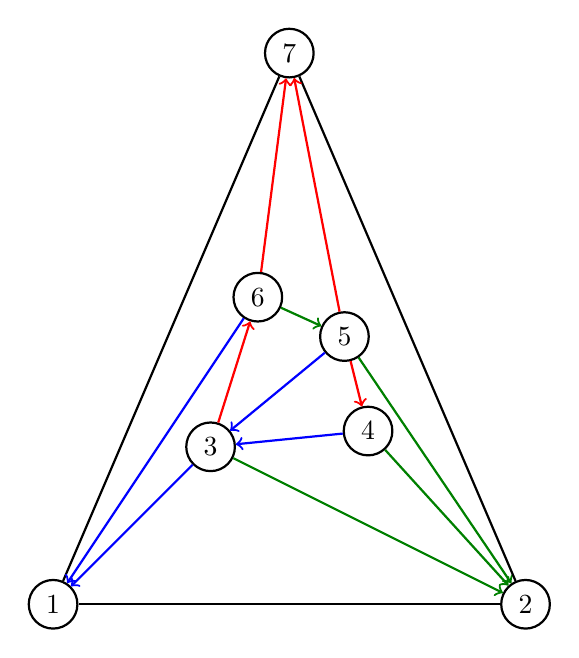
\begin{tikzpicture}[main/.style = {draw, circle, thick}]
			\node[main] (1) at (-1,-1) {1};
			\node[main] (2) at (5,-1) {2};
			\node[main] (3) at (1,1) {3};
			\node[main] (4) at (3, 1.2) {4};
			\node[main] (5) at (2.7, 2.4) {5};
			\node[main] (6) at (1.6, 2.9) {6};
			\node[main] (7) at (2, 6) {7};
			\draw[thick, ->, color=Blue] (3) edge (1);
			\draw[thick] (1) edge (2);
			\draw[thick] (1) edge (7);
			\draw[thick, ->, color=Blue] (6) edge (1);
			\draw[thick, ->, color=Red] (3) edge (6);
			\draw[thick, ->, color=Blue] (4) edge (3);
			\draw[thick, ->, color=Blue] (5) edge (3);
			\draw[thick, ->, color=Green] (3) edge (2);
			\draw[thick, ->, color=Green] (4) edge (2);
			\draw[thick, ->, color=Green] (5) edge (2);
			\draw[thick] (2) edge (7);
			\draw[thick, ->, color=Red] (5) edge (4);
			\draw[thick, ->, color=Green] (6) edge (5);
			\draw[thick, ->, color=Red] (6) edge (7);
			\draw[thick, ->, color=Red] (5) edge (7);
		\end{tikzpicture}
	\end{subfigure}
	\begin{subfigure}{0.45\textwidth}\centering
		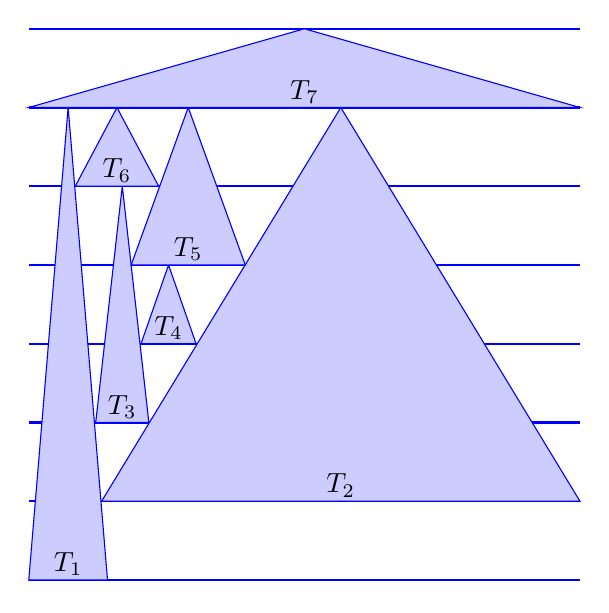
\begin{tikzpicture}
			\draw[Blue, thick] (0,0) -- (7,0);
			\draw[Blue, thick] (0,1) -- (7,1);
			\draw[Blue, thick] (0,2) -- (7,2);
			\draw[Blue, thick] (0,3) -- (7,3);
			\draw[Blue, thick] (0,4) -- (7,4);
			\draw[Blue, thick] (0,5) -- (7,5);
			\draw[Blue, thick] (0,6) -- (7,6);
			\draw[Blue, thick] (0,7) -- (7,7);
			\draw[Blue, fill=Blue!20] (0,0) -- (1,0) -- (0.5,6) -- cycle;
			\draw[Blue, fill=Blue!20] (0.925,1) -- (7,1) -- (3.9625,6) -- cycle;
			\draw[Blue, fill=Blue!20] (0.85,2) -- (1.525,2) -- (1.1875,5) -- cycle;
			\draw[Blue, fill=Blue!20] (1.425,3) -- (2.125,3) -- (1.775,4) -- cycle;
			\draw[Blue, fill=Blue!20] (1.3,4) -- (2.75,4) -- (2.025,6) -- cycle;
			\draw[Blue, fill=Blue!20] (0.59,5) -- (1.65,5) -- (1.12,6) -- cycle;
			\draw[Blue, fill=Blue!20] (0,6) -- (7,6) -- (3.5,7) -- cycle;
			\node at (.5, .2) {$T_1$};
			\node at (3.9625, 1.2) {$T_2$};
			\node at (1.1875, 2.2) {$T_3$};
			\node at (1.775, 3.2) {$T_4$};
			\node at (2.025, 4.2) {$T_5$};
			\node at (1.12, 5.2) {$T_6$};
			\node at (3.5, 6.2) {$T_7$};
		\end{tikzpicture}
	\end{subfigure}
	\caption{An illustration to contact representations by isosceles triangles.}
\end{figure}

\section{Drawing planar graphs on small grids}

\begin{thm}
	Every planar $n$-vertex graph allows a straight-line non-crossing embedding on a grid of size $n \times n$.
\end{thm}

\begin{proof}
	It suffices to prove the theorem for planar triangulations. Given a triangulation $G = (V, E)$, fix an embedding and consider a canonical ordering with respect to this embedding, and run algorithm Schnyder on this canonical ordering. Assign barycentric coordinates $(x_i , y_i , z_i)$ to every vertex $i = 3, 4, \dots, n - 1$ as follows (see Fig. \ref{coord} for illustration): The triangle $12n$ is divided into three regions by the blue, green and red directed paths from $i$ to the roots of the trees in the Schnyder wood. Let $x_i$ be the number of vertices in the region bounded by the blue and green paths and the side $12$, with the vertices on the green path being counted in, but not the vertices of the blue path. Similarly, $y_i$ is the number of vertices in the region bounded by the blue and red paths and the side $1n$, with the vertices on the blue path being counted in, but not the vertices of the red path, and $z_i$ is the number of vertices in the region bounded by the red and green paths and the side $n2$, with the vertices on the red path being counted in, but not the vertices of the green one. Vertex $i$ itself is not counted in neither of the regions.

	\begin{figure}[!ht]\centering
		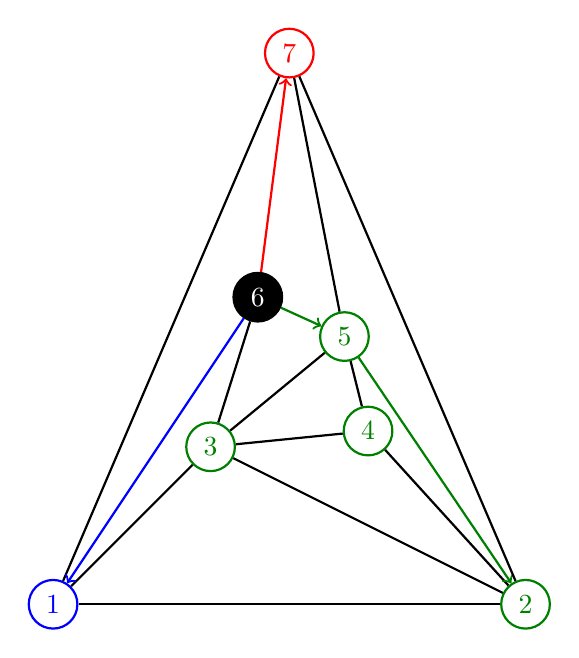
\begin{tikzpicture}[main/.style = {draw, circle, thick}]
			\node[main, Blue] (1) at (-1,-1) {1};
			\node[main, Green] (2) at (5,-1) {2};
			\node[main, Green] (3) at (1,1) {3};
			\node[main, Green] (4) at (3, 1.2) {4};
			\node[main, Green] (5) at (2.7, 2.4) {5};
			\node[main, fill, Black] (6) at (1.6, 2.9) {\textcolor{white}{6}};
			\node[main, Red] (7) at (2, 6) {7};
			\draw[thick] (1) edge (3);
			\draw[thick] (1) edge (2);
			\draw[thick] (1) edge (7);
			\draw[thick, color=Blue, ->] (6) edge (1);
			\draw[thick] (6) edge (3);
			\draw[thick] (4) edge (3);
			\draw[thick] (5) edge (3);
			\draw[thick] (2) edge (3);
			\draw[thick] (2) edge (4);
			\draw[thick, color=Green, ->] (5) edge (2);
			\draw[thick] (2) edge (7);
			\draw[thick] (5) edge (4);
			\draw[thick, color=Green, ->] (6) edge (5);
			\draw[thick, color=Red, ->] (6) edge (7);
			\draw[thick] (7) edge (5);
		\end{tikzpicture}
		\caption{An illustration to the definition of barycentric coordinates from Schnyder woods. The green vertices are counted for the definition of $x_6$, the blue one for the definition of $y_6$ and the red one for the definition of $z_6$. Vertex 6 itself does not contribute to any of the coordinates.}
		\label{coord}
	\end{figure}

	Then every vertex except of $i$ belongs to exactly one of the regions, end hence
	
	$$
	x_i + y_i + z_i = n - 1
	$$
	
	for every $i$. For $i = 1, 2$, and $n$, we set
	
	$$
	\begin{array}{lll}
		x_1 = 0,   &y_1 = 0,   &z_1 = n - 1\\
		x_2 = 0,   &y_2 = n-1, &z_2 = 0\\
		x_n = n-1, &y_n = 0,   & z_n = 0 	
	\end{array}
	$$
	
	Place vertex $i$ in the point with barycentric coordinates $(x_i , y_i , z_i)$ in a triangular $n \times n \times n$ grid (the lines of the grid have coordinates $0, 1, \dots, n - 1$). Draw the edges of $G$ as straight-line segments
	connecting their vertices.
	
	\begin{claim}
		Consider a vertex $i \in \{3, 4, \dots, n - 1\}$. In the drawing constructed as above, the blue edge $ib(i)$ is directed into the bottom-left sextant of $i$, the edge $ig(i)$ is directed into the bottom-right sextant of $i$, and the edge $ir(i)$ is directed into the top sextant of $i$.
		\label{claim-1}
	\end{claim}
	
	\begin{proof}[Proof of claim]
		From the definition of the coordinates, it follows that $xb(i) \leq x_i$, $yb(i) < y_i$ and $zb(i) \geq z_i$, and this implies the direction of the edge $ib(i)$. Similarly for the others.
	\end{proof}
	
	\begin{claim}
		The rotation scheme of the edges around each vertex $i$ in the barycentric drawing is the same as the rotation scheme of the edges incident to the same vertex in $G$.
	\end{claim}
	
	\begin{proof}[Proof of claim]
		This follows by application of Claim \ref{claim-1} to the other end-vertices of the edges directed into $i$.
	\end{proof}
	
	\begin{claim}
		The barycentric drawing is non-crossing and topologically equivalent to the plane embedding of $G$ we started with.
	\end{claim}
	
	\begin{proof}[Proof of claim]
		If the rotation schemes for all vertices of drawings of two 3-connected graphs are the same and one of the drawings is non-crossing, then so is the other one, and the drawings are topologically equivalent.
	\end{proof}
\end{proof}

\section{Boxicity of graphs}

\begin{defn}
	The \textbf{boxicity} of a graph $G$, denoted by $\text{box}(G)$, is the smallest integer $d$ such that $G$ is an intersection graph of boxes in $\R^d$ (i.e., of $d$-dimensional intervals in the $d$-dimensional Euclidean space).
\end{defn}

\begin{prop}
For every graph $G = (V, E)$, its boxicity is a correctly defined finite number. It equals the minimum number of interval graphs whose intersection is equal to $G$, i.e., the minimum number $d$ for which sets $E_i \subseteq \binom{V}{2} , i = 1, 2, \dots, d$ exist, such that $E = \cup_{i=1}^d E_i$ and $(V, E_i)$ is an interval graph for every $i = 1, 2, \dots, d$.
\end{prop}

\begin{proof}
	An exercise. Proof the claim for graphs $G$ which are not complete. For a complete graph, the boxicity is $0$, which corresponds to the fact that the intersection of an empty set of subsets of a ground set ($E$, in this case) is by default set to be equal to the ground set itself.
\end{proof}

\section{Grid intersection graphs}

\begin{defn}
	A graph is a \textbf{Grid Intersection graph} if it has an intersection repre-\\sentation by vertical and horizontal segments in which no two segments of the same direction share a point (in other words, all vertical, as well as all horizontal, segments are pairwise disjoint).
\end{defn}

It is easy to observe that every grid intersection graph has a grid intersection repre-\\sentation in which no two segments lie on the same line. Moreover, the exact $x$-coordinates of the vertical segments, nor the exact $y$-coordinates of the horizontal ones, are important, only their linear orders. Thus we assume that our bipartite graph $G = (A \cup B, E)$ has its vertices linearly ordered within the classes of bipartition, $A = \{a_1 , a_2 , \dots, a_n\}, B = \{b_1 , b_2 \dots, b_m\}$. We further assume that the vertices of $A$ are to be represented by vertical segments and the vertices of $B$ by horizontal ones. We say that a grid intersection representation respects the orders of $A$ and $B$ if for every $i < j$, the $x$-coordinate of $a_i$ is smaller than the $x$-coordinate of $a_j$, and the $y$-coordinate of $b_i$ is smaller than the $y$-coordinate of $b_j$.

\begin{thm}
	The graph $G = (A \cup B, E)$ has a grid intersection representation that respects the linear orders of $A$ and $B$ if and only if there are no 6 indices $i < j < k, \alpha < \beta < \gamma$ such that $a_i b_\beta , a_k b_\beta , a_j b_\alpha , a_j b_\gamma$ are edges of $G$ and $a_j b_\beta$ is not. Such a configuration of 6 vertices is called a \textbf{volswagen} in $G$.
	\label{thm-5}
\end{thm}

\begin{proof}
	Exercise.
\end{proof}

It is easy (i.e., decidable in polynomial time) to check if a bipartite graph contains a volkswagen with respect to given linear orderings of the vertices in its classes of bipartition. We will see in the last class that it is NP-complete to decide if a given bipartite graph is a grid intersection graph, which means that it is NP-complete to decide if a given bipartite graph allows linear orderings of its classes of bipartition with respect to which there is no volkswagen. The following problem is thus quite interesting in this context.

\textbf{Open problem:} Given a bipartite graph with one class of bipartition linearly ordered. How difficult is to decide if the other class of bipartition can be linearly ordered so that there is no volkswagen with respect to these orderings?

\begin{thm}[Bellantoni, Hartman, Przytycka, Whitesides]
	Every bipartite graph of boxicity $2$ is a grid intersection graph.
\end{thm}

\begin{figure}[!ht]\centering
	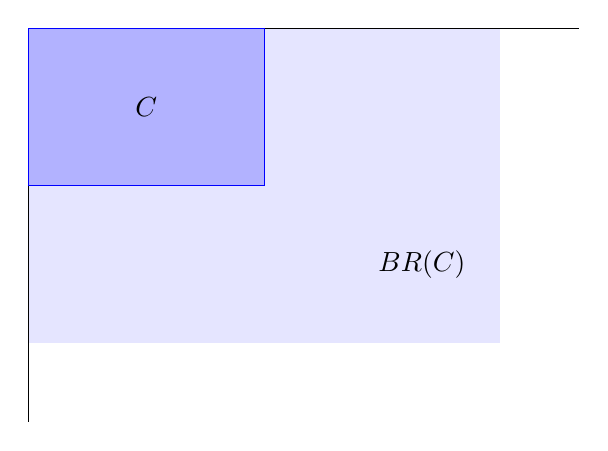
\begin{tikzpicture}
		\draw[black!0, fill=blue!10] (0,-2) rectangle (6,2);
		\draw (0,2) -- (7,2);
		\draw (0,2) -- (0, -3);
		\draw[blue, fill=blue!30] (0,0) rectangle (3,2);
		\node at (1.5, 1) {$C$};
		\node at (5,-1) {$BR(C)$};
	\end{tikzpicture}
	\caption{An illustration to the definition of region $BR(C)$.}
\end{figure}

\begin{proof}[Sketch of proof]
	Suppose $G = (A \cup B, E)$ is a bipartite graph and let $\mathcal{R} = \{R(u) : u \in A \cup B\}$ be an intersection representation of $G$ by axes-parallel rectangles in the plane. For a rectangle $C$ in the plane, we define regions $BL(C)$, $BR(C)$, $TL(C)$, $TR(C)$ as follows: $BR(C)$ contains all points with $x$-coordinate greater than the $x$-coordinate of the left side of $C$, with $y$-coordinate smaller than the $y$-coordinate of the top side of $C$, but which do not lie inside the rectangle $C$. The other regions ($BL$ standing for Bottom-Left, $TL$ standing for Top-Left, and $TR$ standing for Top-Right) are defined in a similar way. Then define two binary relations, one on $A$, the other one on $B$, as follows
	
	$$
	\begin{array}{c c c c}
		a_1 <_R a_2 & \Leftrightarrow & R(a_1) \cap BR(R(a_2)) \neq \emptyset & \text{ for } a_1, a_2 \in A, \\
		b_1 <_R b_2 & \Leftrightarrow & R(b_1) \cap BL(R(b_2)) \neq \emptyset & \text{ for } b_1, b_2 \in B. \\
	\end{array}
	$$
	
	\begin{claim}
		Both relations $<_R$ and $<_L$ are antireflexive, antisymmetric and acyclic. It follows that the transitive closures $<_{R}^T$ and $<_{L}^T$ of $<_R$ and $<_L$, respectively, are partial orders.
	\end{claim}
	
	Let $<_R^\ast$ and $<_L^\ast$ be topological sortings of $<_R^T$ and $<_L^T$, respectively.
	
	\begin{claim}
		With respect to the linear orderings $<_R^\ast$ and $<_L^\ast$ of its classes of bipartition, $G$ has no volkswagens. Hence $G$ has a grid intersection representation respecting these orders by Theorem \ref{thm-5}.
	\end{claim}
\end{proof}
	\chapter{String graphs}

\begin{defn}
	String graphs are intersection graphs on arbitrary lines in plane.
\end{defn}

\begin{defn}
	\textbf{OuterString} class is a class of graphs which are represented by inter-\\section graphs of lines starting from a circle boundary and growing arbitrarily inside the circle. Then \textbf{constrained outer strings} is class containing graphs that are outer strings but also it is determined the order of lines appearance on the circle.
\end{defn}

\TODO{Create some pictures.}

\begin{thm}
	For $n \geq 4$ the complement of $C_n$, $-C_n \notin$ constrained-outerstring.
\end{thm}

\begin{proof}
	We proceed by induction on $n$. First we start by $n = 4$. Where if we draw the graph and because on the circle the two opposite nodes have to connect somewhere, but not cross any other. That is impossible.
	
	For greater $n > 4$ suppose for contrary that $-C_n$ has a representation. Take such with smallest number of crossing number. Then we create two more graphs $-C_{i+1} = -C_n[1,2, \dots, i]$ and $-C_{n-1+1} = -C_n[i, i+1, \dots, n]$ since $n \geq 5$ both have size at least $4$ but less than the $-C_n$ but we know that one of them don't have a representation.
\end{proof}

\begin{thm}
	Recognition of STRING is NP-hard.
\end{thm}

\begin{proof}
	The proof is done by creating a transformation of Planar 3-SAT to RECOG\\(STRING). We won't go deeper into the proof, but shortly as usual you create some gadgets for variables and for clauses. Then you need to bind them. After that you use the planarity of 3-SAT to create a graph that is representable as a STRING graph only if the SAT is satisfied. That is it abuses the previously mentioned theorem.
	
	Also it can be done by straight lines. Therefore also recognition of $GI$ is NP-complete.
\end{proof}

\begin{thm}
	RECOG(SEG), RECOG(CONV) are in $\exists \R \subseteq$ PSPACE.
\end{thm}

This can be proven by the following $\exists \R$ problem. We ar egiven $n$ polynoms $p_1, \dots, p_n$ for $n$ variables $x_1, \dots, x_n$. The question is then whether there exists such assignment to $x_1, \dots, x_n \in \R$ that all polynoms are non-negative.

\begin{proof}
	We will represent $G$ for each $u \in V(G)$ as $M_u$ convex set. Then we set points $\forall uv \in E(G) : P_{uv} = (x_{uv}, y_{uv})$. After that we take a convex hull of all inner points. Therefore we denote $M'_u = \text{conv}(P_{uv}| v \in N_G(v))$. Now $(M_u' | u \in V(G))$ is convex reprezentation of $G$.
	
	If $M_u \cap M_v \neq \emptyset \Rightarrow P_uv \in M_u' \cap M_v' \neq \emptyset$ if $uv \notin E(G)$ there exists a line separating these two convex hulls. This line can be prescribed as a polynom. Therefore these polynoms must be negative for all non-edges.
	
	For the RECOG(SEG) we may use similiar trick.
\end{proof}

\begin{comm}
	If $G \in$ STRING then mwe must find such lines instead of nodes, but if we pick points representing edges then the graph is planar. So we must guess such planar graph $H$ and then the paths. But this is not enough for NP since the polynomial is dependent on the size of the unknown $H$.
\end{comm}

\begin{defn}
	$\text{STR}(n)$ is min $k$ such that $\forall G \in$ STRING $|V(G)| =n$  there exists STRING representation with at most $k$ crossing points.
\end{defn}

\begin{defn}
	$AT$-graf is $(G = (V,E), R \subset \binom{E}{2})$ and it is (weakly) realisable if there exists drawing $D$ of a graph $G$ in the plane s.t. $\forall e,f \in E(G): D_e \cap D_f \neq \emptyset \Rightarrow \{e,f\} \in R$.
\end{defn}

\begin{observ}
	$R = \emptyset$ then $(G, \emptyset)$ is realisable iff $G$ is planar.
\end{observ}

\begin{defn}
	$\text{AT}(n)$ is min $k$ s.t. $\forall$ realisable $AT$-graf with $n = |E(G)|$ is realisable with at most $k$ crossing points.
\end{defn}

\begin{thm}
	$\text{STR}(n) \sim \text{AT}(n)$.
\end{thm}

\begin{proof}
	"$\Rightarrow$" Let $G \in$ STRING and $|V(G)| = n, G$ needs $\text{STR}(n)$ crossing points. Lets take such representation $\forall u,v \in V(G)$ where $u \neq v$ and $uv \in E(G)$ we select point $P_{uv} \in S_u \cap S_v$ and say that these are nodes of the new graph $G'$. $S_u$ is a line representing $U \in V(G)$.
	
	\TODO{finish the proof}
\end{proof}

\begin{thm}
	$\text{AT}(n) \geq 2^{cn}$ for constant $c$.
\end{thm}

\begin{proof}
	We will create a certain type of a graph depicted on the picture. %\ref{}.
	
	\TODO{Finsih the proof and create a picture.}
\end{proof}

\begin{thm}
	RECOG(STRING) $\in$ NP.
\end{thm}

This will be shown in the second part of this course.

\begin{thm}
	$\text{AT}(n) \leq n \cdot 2^n$.
\end{thm}

\TODO{Finish the proof and also state supporting lemma.}
	\part{Geometric Representations of Graphs II}
	\chapter{STRING $\in$ NP}

Now we will take a look at recognition of STRING graphs. Mainly that this problem is indeed in NP. We have already shown in the first part that STRING-recognition is NP-hard. The main problem is that some string graphs require representation with exponentially many crossings. Which is not possible to guess in an NP algorithm.

Also we have shown (Schaeffer and Štěfanovič) result that any string graph has a representation with at most exponentially many crossings.

Before we continue lets give us an example of a graph and its STRING representation which can be seen on Fig. \ref{string example}.

\begin{figure}[!ht]\centering
	\begin{subfigure}{.45\textwidth}\centering
		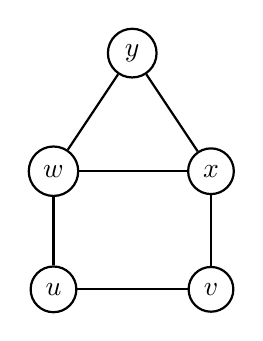
\begin{tikzpicture}[main/.style = {draw, circle, thick}]
			\node[main] (u) at (0,0) {$u$};
			\node[main] (v) at (2,0) {$v$};
			\node[main] (w) at (0,1.5) {$w$};
			\node[main] (x) at (2,1.5) {$x$};
			\node[main] (y) at (1,3) {$y$};
			\draw[thick] (u) -- (v);
			\draw[thick] (u) -- (w);
			\draw[thick] (v) -- (x);
			\draw[thick] (w) -- (x);
			\draw[thick] (w) -- (y);
			\draw[thick] (x) -- (y);
		\end{tikzpicture}
		\caption{Graph $G$.}
	\end{subfigure}
	\begin{subfigure}{.45\textwidth}\centering
		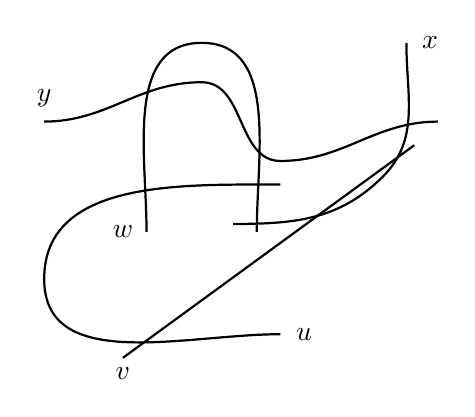
\begin{tikzpicture}
			\draw[thick] (-1,0) to[out=0, in=180] (1,.5) to[out=0, in=180] (2,-.5) to[out=0, in=180] (4,0);
			\node at (-1,.3) {$y$};
			\draw[thick] (.3, -1.4) to[out=90, in=180] (1,1) to[out=0, in=90] (1.7, -1.4);
			\node at (0, -1.4) {$w$};
			\draw[thick] (2, -0.8) to[out=180, in=90] (-1, -2) to[out=270, in=180] (2, -2.7);
			\node at (2.3, -2.7) {$u$};
			\draw[thick] (1.4, -1.3) to[out=0, in=225] (3.3, -.7) to[out=45, in=270] (3.6, 1);
			\node at (3.9, 1) {$x$};
			\draw[thick] (0, -3) to (3.7, -.3);
			\node at (0, -3.2) {$v$};
		\end{tikzpicture}
		\caption{String representation.}
	\end{subfigure}
	\caption{Example of a STRING graph.}
	\label{string example}
\end{figure}

Firstly lets define another problem which can be converted from STRING-recognition.

\section{Weak AT-realization}

The \textbf{INPUT} is a graph $G = (V,E)$ and $R \subseteq \binom{E}{2}$. The \textbf{GOAL} is to find a drawing of $G$ where only the pairs of edges from $R$ are allowed to cross.

Note that AT stands for abstract topological and weak means that the pairs do \textbf{not hove} to cross, only they can.

For now the drawing is somewhat basic. That is no edges crosses through a vertex. Vertices are points and edges are curves.

\section{Reduction of STRING-recognition to Weak AT-realization}

For a given graph $G = (V_G,E_G)$ we define the following graph $H = (V_H, E_H)$ and $R$. $V_H = V_G \cup E_G$ and $E_H = \{\{v,e\}, v \in V_G, e \in E_G, v \in e\}$. Lets see an example on Fig. \ref{reduction of strings}. We may see that the graph is obtained by subdividing all edges.

\begin{figure}[!ht]\centering
	\begin{subfigure}{.45\textwidth}\centering
		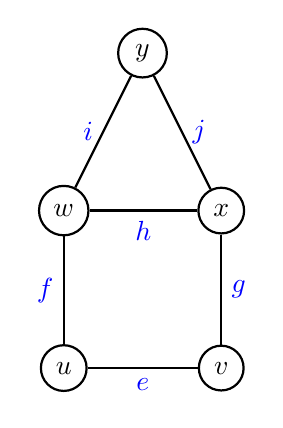
\begin{tikzpicture}[main/.style = {draw, circle, thick}, e/.style = {Blue}]
			\node[main] (u) at (0,0) {$u$};
			\node[main] (v) at (2,0) {$v$};
			\node[main] (w) at (0,2) {$w$};
			\node[main] (x) at (2,2) {$x$};
			\node[main] (y) at (1,4) {$y$};
			\draw[thick] (u) -- (v) node[midway, e, below] {$e$};
			\draw[thick] (u) -- (w) node[midway, e, left] {$f$};
			\draw[thick] (v) -- (x) node[midway, e, right] {$g$};
			\draw[thick] (w) -- (x) node[midway, e, below] {$h$};
			\draw[thick] (w) -- (y) node[midway, e, above, left] {$i$};
			\draw[thick] (x) -- (y) node[midway, e, above, right] {$j$};
		\end{tikzpicture}
		\caption{Original graph $G$.}
	\end{subfigure}
	\begin{subfigure}{.45\textwidth}\centering
		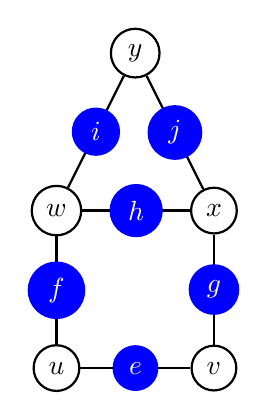
\begin{tikzpicture}[main/.style = {draw, circle, thick}, e/.style = {draw, circle, fill, Blue}]
			\node[main] (u) at (0,0) {$u$};
			\node[main] (v) at (2,0) {$v$};
			\node[main] (w) at (0,2) {$w$};
			\node[main] (x) at (2,2) {$x$};
			\node[main] (y) at (1,4) {$y$};
			\draw[thick] (u) -- (v) node[midway, e] {\textcolor{white}{$e$}};
			\draw[thick] (u) -- (w) node[midway, e] {\textcolor{white}{$f$}};
			\draw[thick] (v) -- (x) node[midway, e] {\textcolor{white}{$g$}};
			\draw[thick] (w) -- (x) node[midway, e] {\textcolor{white}{$h$}};
			\draw[thick] (w) -- (y) node[midway, e] {\textcolor{white}{$i$}};
			\draw[thick] (x) -- (y) node[midway, e] {\textcolor{white}{$j$}};
		\end{tikzpicture}
		\caption{Graph $H$.}
	\end{subfigure}
	\caption{Creating $H$ from $G$.}
	\label{reduction of strings}
\end{figure}

Lastly we define $R = \{\{\{v, e\}, \{w,f\}\}, \{v,w\} \in E_G\}$.

\begin{claim}
	$G$ is a STRING graph $\Leftrightarrow$ $(H,R)$ has Weak AT-realization.
\end{claim}

\begin{proof}
	"$\Rightarrow$" Suppose $G$ is a STRING graph. Pick endpoints as vertices and crossings as edge-vertices of $H$. Choose these arbitrary (see Fig. \ref{rightarrow} for an example). The edges will follow the lines in a STRING representation.
	
	"$\Leftarrow$" Suppose $(H,R)$ has a Weak AT-realization. See that $H$ is bipartite. Now represent it by going from the vertex alongside every edge to the edge-vertices of $H$ and almost return to the vertex. See Fig. \ref{leftarrow} for an example. It is easily observable that when lines cross then indeed they need be connected by an edge.
	
	\begin{figure}[!ht]\centering
		\begin{subfigure}{.4\textwidth}\centering
				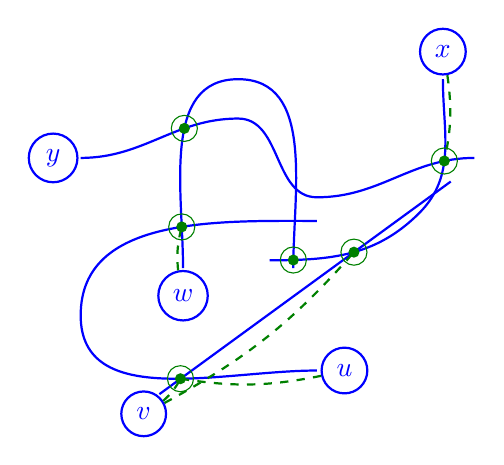
\begin{tikzpicture}[main/.style = {draw, circle, thick, Blue}, c/.style = {thick, Blue},
					side/.style = {draw, circle, thick, Green}]
					\draw[c,name path=A] (-1,0) to[out=0, in=180] (1,.5) to[out=0, in=180] (2,-.5) to[out=0, in=180] (4,0);
					\node[main] at (-1.35,0) (y) {$y$};
					\draw[c,name path=B] (.3, -1.4) to[out=90, in=180] (1,1) to[out=0, in=90] (1.7, -1.4);
					\node[main] at (.3, -1.75) (w) {$w$};
					\draw[c,name path=C] (2, -0.8) to[out=180, in=90] (-1, -2) to[out=270, in=180] (2, -2.7);
					\node[main] at (2.35, -2.7) (u) {$u$};
					\draw[c,name path=D] (1.4, -1.3) to[out=0, in=225] (3.3, -.7) to[out=45, in=270] (3.6, 1);
					\node[main] at (3.6, 1.35) (x) {$x$};
					\draw[c,name path=E] (0, -3) to (3.7, -.3);
					\node[main] at (-.2, -3.25) (v) {$v$};
					% Intersections and dots
					\coordinate[name intersections={of=A and B, by=ab}];
					\fill[Green] (ab) circle (2pt) node[circle,draw] {};
					\coordinate[name intersections={of=A and D, by=ad}];
					\fill[Green] (ad) circle (2pt) node[circle,draw] {};
					\coordinate[name intersections={of=B and C, by=bc}];
					\fill[Green] (bc) circle (2pt) node[circle,draw] {};
					\coordinate[name intersections={of=B and D, by=bd}];
					\fill[Green] (bd) circle (2pt) node[circle,draw] {};
					\coordinate[name intersections={of=C and E, by=ce}];
					\fill[Green] (ce) circle (2pt) node[circle,draw] {};
					\coordinate[name intersections={of=D and E, by=de}];
					\fill[Green] (de) circle (2pt) node[circle,draw] {};
					\draw[dashed, thick, Green, bend right = 10] (v) edge (ce);
					\draw[dashed, thick, Green, bend left = 10] (u) edge (ce);
					\draw[dashed, thick, Green, bend right = 10] (v) edge (de);
					\draw[dashed, thick, Green, bend left = 10] (w) edge (bc);
					\draw[dashed, thick, Green, bend left = 10] (x) edge (ad);
				\end{tikzpicture}
			\caption{$\Rightarrow$ (Only some edges are present.)}
			\label{rightarrow}
		\end{subfigure}
		\begin{subfigure}{.58\textwidth}\centering
			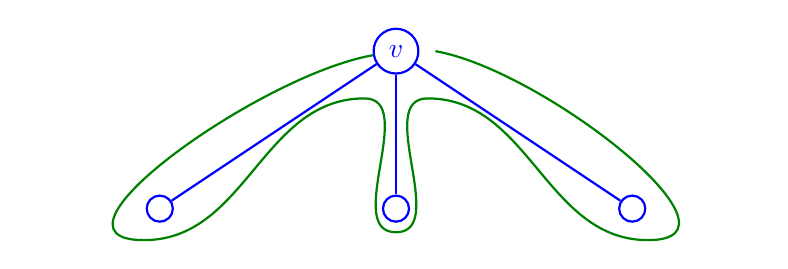
\begin{tikzpicture}[main/.style = {draw, circle, thick, Blue}]
				\node[main] at (0,0) (v) {$v$};
				\node[main] at (-3, -2) (1) {};
				\node[main] at (0, -2) (2) {};
				\node[main] at (3, -2) (3) {};
				\draw[thick, Blue] (v) to[] (1);
				\draw[thick, Blue] (v) to[] (2);
				\draw[thick, Blue] (v) to[] (3);
				\draw[thick, Green] (v) to[out=190, in=180] (-3.2, -2.4) to[out=0, in=180] (-.4,-.6) to[out=0, in=180] (0, -2.3) to[out=0, in=180] (.4,-.6) to[out=0, in=180] (3.2, -2.4) to[out=0, in=-10] (.5, 0);
			\end{tikzpicture}
			\caption{$\Leftarrow$}
			\label{leftarrow}
		\end{subfigure}
		\caption{Examples for the proof.}
	\end{figure}
\end{proof}

\subsection{Test Weak AT-realization in NP}

Firstly we will write down all our assumption about the drawing we will be using.

\begin{enumerate}
	\item We are on the sphere.
	\item Vertex $v$ is drawn as an open disc $D_v$ (also we will denote $\partial D_v$ as the boundary of $D_v$ and $\overline{D_v}$ as the closure of $D_v$, i.e. $\overline{D_v} = D_v \cup \partial D_v$).
	\item An edge $e = \{v,w\}$ is represented by a curve $\gamma_e$ connecting a point from $\partial D_v$ to a point from $\partial D_w$ otherwise $\gamma_e$ is disjoint from $\bigcup_{x \in V} \overline{D_x}$.
	\item For $e \neq f$ $\gamma_e$ and $\gamma_f$ have distinct endpoints.
\end{enumerate}

We can easily see that these assumption are not restricting since it can be switch to "normal" drawing we are using by shrinking the discs to single points and switch back by expanding the single points.

Now we will proceed with the first part of the algorithm \ref{}.

\begin{algorithm}[!ht]
	\begin{algorithmic}[1]
		\Require $G = (V,E), R \subseteq \binom{E}{2}$
		\State $\forall v \in V:$ choose $D_v$ (so that $v \neq w$ have $\overline{D_v} \cap \overline{D_w} = \emptyset$).
		\State For any edge $e \in E$ incident to $v \in V:$ choose an endpoint of $\gamma_e$ on $\partial D_v$.
		\State \textcolor{Green}{$\dots$}
	\end{algorithmic}
	\caption{NP algorithm for testing Weak AT-realization.}
	\label{AT-1}
\end{algorithm}

Before we continue with the algorithm we will take a short topological detour to some definitions and facts.

\subsection{Topological detour}

\begin{defn}
	$\mathcal{S} := (\text{sphere}) \setminus \bigcup_{v \in V} D_v$. Which is a compact surface with boundary.
\end{defn}

\begin{defn}
	$\mathcal{S}-\text{curve}$ is a curve in $\mathcal{S}$ with endpoints in the $\partial \mathcal{S}$ and no other point in $\partial \mathcal{S}$.
\end{defn}

\begin{defn}
	Two $\mathcal{S}$-curves $\gamma, \delta$ are \textbf{isotopic} (written as $\gamma \sim \delta$) if $\gamma$ and $\delta$ have the same endpoints and $\gamma$ can be transformed into $\delta$ by a continuous deformations of $\mathcal{S}$ which fixes the boundary.
\end{defn}

\begin{figure}[!ht]\centering
	\begin{subfigure}{.45\textwidth}\centering
		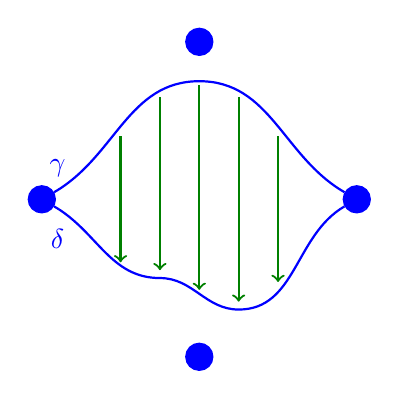
\begin{tikzpicture}[main/.style = {draw, circle, thick, fill, Blue}]
			\node[main] (0) at (0,2) {};
			\node[main] (1) at (-2,0) {};
			\node[main] (2) at (2,0) {};
			\node[main] (3) at (0, -2) {};
			\draw[thick, Blue] (1) to[out=30, in=180] (0,1.5) to[out=0, in=150] (2);
			\node[blue] (gamma) at (-1.8, .4) {$\gamma$};
			\draw[thick, Blue] (1) to[out=-30, in=180] (-.5,-1) to[out=0, in=180] (.5, -1.4) to[out=0, in=210] (2);
			\node[blue] (delta) at (-1.8, -.5) {$\delta$};
			\draw[thick, Green, ->] (0, 1.45) to[] (0,-1.15);
			\draw[thick, Green, ->] (-1, .8) to[] (-1,-.8);
			\draw[thick, Green, ->] (-.5, 1.3) to[] (-.5,-.9);
			\draw[thick, Green, ->] (.5, 1.3) to[] (.5,-1.3);
			\draw[thick, Green, ->] (1, .8) to[] (1,-1.05);
		\end{tikzpicture}
		\caption{Example of $\mathcal{S}$-curves $\gamma, \delta$ that are isotopic.}
	\end{subfigure}
	\begin{subfigure}{.45\textwidth}\centering
		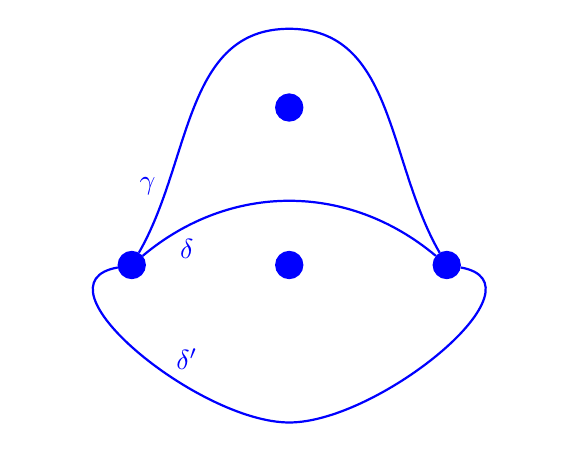
\begin{tikzpicture}[main/.style = {draw, circle, thick, fill, Blue}]
			\node[main] (0) at (0,2) {};
			\node[main] (1) at (-2,0) {};
			\node[main] (2) at (2,0) {};
			\node[main] (3) at (0, 0) {};
			\draw[thick, Blue] (1) to[out=40, in=140] (2);
			\node[blue] (gamma) at (-1.8, 1) {$\gamma$};
			\draw[thick, Blue] (1) to[out=60, in=180] (0,3) to[out=0, in=120] (2);
			\node[blue] (delta) at (-1.3, .2) {$\delta$};
			\draw[thick, Blue] (1) to[out=190, in=180] (0,-2) to[out=0, in=350] (2);
			\node[blue] (deltap) at (-1.3, -1.2) {$\delta'$};
		\end{tikzpicture}
		\caption{Counterexample of non-isotopic $\gamma \not \sim \delta$ and example of isotopic $\gamma \sim \delta'$.}
	\end{subfigure}
	\caption{Example of isotopic and non-isotopic $\mathcal{S}$-curves.}
\end{figure}

\begin{defn}
	For two $\mathcal{S}$-curves $\gamma_1, \gamma_2$ the intersection number $i(\gamma_1, \gamma_2)$ is
	
	$$
	\min_{\delta_1 \sim \gamma_1, \delta_2 \sim \gamma_2} |\delta_1 \cap \delta_2|.
	$$
\end{defn}

\begin{fact}
	Let $\gamma_1, \dots, \gamma_n$ be $\mathcal{S}$-curves. Then there are $\mathcal{S}$-curves $\delta_1, \dots, \delta_n$ s.t.
	
	\begin{enumerate}
		\item $\delta_i \sim \gamma_i$ for $i = 1, \dots, n$,
		\item $|\delta_i \cap \delta_j| = i(\gamma_i, \gamma_j)$ for $i \neq j \in \{1, \dots, n\}$. 
	\end{enumerate}
\end{fact}

\noindent
With all these definitions we will choose the following triangulation $T = (V_T, E_T)$ of $\mathcal{S}$:

\begin{enumerate}
	\item $\forall v \in V: \partial D_v$ has three vertices and three edges of $T$.
	\item There are no other vertices of $T$, the remaining edges are chosen arbitrarily as $\mathcal{S}$-curves, so that $\mathcal{S}$ is partitioned into triangle faces.
	\item Vertices of $T$ do not coincide with endpoints of $\gamma_e, e \in E$ from algorithm.
\end{enumerate}

\begin{defn}
	An $\mathcal{S}$-curve $\gamma$ is \textbf{normal} w.r.t. T if
	
	\begin{enumerate}
		\item The endpoints of $\gamma$ are distinct from $V_T$.
		\item Any point where an edge of $T$ meets $\gamma$ is either an endpoint of $\gamma$ or a proper crossing (no touching is allowed).
		\item $\gamma$ does not have two consecutive crossings with any edge of $T$.
		\item $\gamma$ does not cross the same edge of $T$ no more than $2^{|E_T| + |E|}$-times.
	\end{enumerate}
\end{defn}

\begin{claim}
	If $G$ has a weak AT-realization, then it has a realization where each $\gamma_e$ is normal w.r.t. T.
\end{claim}

\begin{proof}
	Take AT with minimum number of crossings. 1. is satisfied by the definition. 2. otherwise minimality is broken, 3. again the minimality is broken and lastly 4. follows from GRG1.
	
	\begin{figure}[!ht]\centering
		\begin{subfigure}{.2\textwidth}\centering
			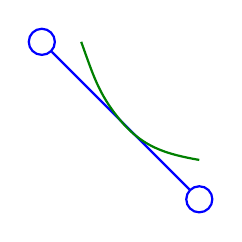
\begin{tikzpicture}[main/.style = {draw, circle}, e/.style = {thick, Blue}]
				\node[main,e] at (0,0) (0) {};
				\node[main,e] at (-2,2) (1) {};
				\draw[e] (0) -- (1);
				\draw[thick, Green] (0, .5) to[out=170, in=310] (-1,1) to[out=130,in=290] (-1.5,2);
			\end{tikzpicture}
			\caption{Second before.}
		\end{subfigure}
		\begin{subfigure}{.2\textwidth}\centering
			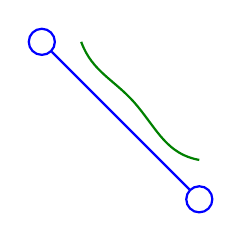
\begin{tikzpicture}[main/.style = {draw, circle}, e/.style = {thick, Blue}]
				\node[main,e] at (0,0) (0) {};
				\node[main,e] at (-2,2) (1) {};
				\draw[e] (0) -- (1);
				\draw[thick, Green] (0, .5) to[out=170, in=310] (-.8,1.2) to[out=130,in=290] (-1.5,2);
			\end{tikzpicture}
			\caption{Second after.}
		\end{subfigure}
		\begin{subfigure}{.2\textwidth}\centering
			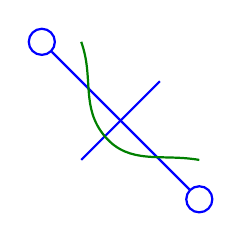
\begin{tikzpicture}[main/.style = {draw, circle}, e/.style = {thick, Blue}]
				\node[main,e] at (0,0) (0) {};
				\node[main,e] at (-2,2) (1) {};
				\draw[e] (0) -- (1);
				\draw[e] (-1.5,.5) -- (-.5,1.5);
				\draw[thick, Green] (0, .5) to[out=170, in=310] (-1.2,.8) to[out=130,in=290] (-1.5,2);
			\end{tikzpicture}
			\caption{Third before.}
		\end{subfigure}
		\begin{subfigure}{.2\textwidth}\centering
			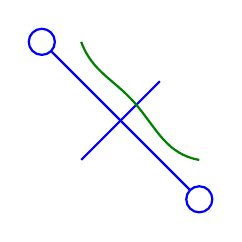
\begin{tikzpicture}[main/.style = {draw, circle}, e/.style = {thick, Blue}]
				\node[main,e] at (0,0) (0) {};
				\node[main,e] at (-2,2) (1) {};
				\draw[e] (0) -- (1);
				\draw[e] (-1.5,.5) -- (-.5,1.5);
				\draw[thick, Green] (0, .5) to[out=170, in=310] (-.8,1.2) to[out=130,in=290] (-1.5,2);
			\end{tikzpicture}
			\caption{Third after.}
		\end{subfigure}
		\caption{Examples for the proof.}
	\end{figure}
\end{proof}

\begin{defn}
	Let $\gamma$ be an $\mathcal{S}$-curve, normal w.r.t T for $e \in E_T: c_e(\gamma) := |e \cap \gamma|$.
\end{defn}

Sometimes when we will be talking about $\gamma_e$ for some $e \in E$ then for $f \in E_T$ we will denote $c_f(e)$ as $c_f(\gamma_e)$. Also in the context we will sometimes leave out $\gamma_e$ and only have $c_f$ or $c_{uv}$ if $f = \{u,v\}$. 

\begin{claim}
	The numbers $\left( c_f(e)\right)_{f \in E_T}$ determine $\gamma_e$ up to isotopy.
	\label{string-claim}
\end{claim}

\subsection{Word equations}

Before we showcase the proof we will show us a quick introduction to word algebra and its equations. We will be considering a finite alphabet $\mathcal{A} = \{\mathtt{a}, \mathtt{b}, \mathtt{c}, \dots\}$ and variables $\mathcal{V} = \{X,Y, \dots\}$. Each variable $X \in V$ has prescribed length $l(X) \in \N_0$ and represents a word over $\mathcal{A}$ of length $l(X)$.

\begin{example}
	$\mathcal{A} = \{\mathtt{a}, \mathtt{b}\}, \mathcal{V} = \{X,Y\}, l(X) = 2, l(Y) = 3$ and the equation is:
	
	$$
	XX\mathtt{a} = XY,
	$$
	
	\noindent where the operation is concatenation. One simple solution is $X := \mathtt{ba}$ and $Y := \mathtt{baa}$.
\end{example}

We may see that having one equation or a whole system of equation is the same. As we can see here:

$$
\begin{array}{c c c}
	L_1 = R_1 & & \\
	L_2 = R_2 & \Leftrightarrow & L_1L_2 \dots = R_1 R_2 \dots \\
	\vdots & &
\end{array}
$$

Also it may be that the size of a solution can be even exponential. But there is usually a repeating pattern. We can examine the following example to see that it is indeed true.

$$
\begin{array}{r c l}
	X_1 &=& \mathtt{a} \\
	X_2 &=& X_1 X_1 \\
	X_3 &=& X_2 X_2 \\
	&\vdots&
\end{array}
$$

\begin{fact}
	There is an encoding ("LZ-encoding") such that for any system of word equations we can in \textbf{polynomial time} (in $\abs{\mathcal{A}} + \abs{\mathcal{V}} + \abs{\text{equations}} + \abs{\sum_{X \in \mathcal{V}} \log |l(X)|}$) determine if a solution exists and compute the LZ-encoding of the lexicographically smallest solution.
\end{fact}

\begin{fact}
	From the LZ-encoding of a word $X \in \mathcal{A}^{\ast}$ we can compute the number of occurrences of any symbol $\mathtt{a} \in \mathcal{A}$ in $X$.
\end{fact}

\subsubsection{LZ-encoding}

Shortly we will talk about the exact LZ-encoding. Firstly for a word $\mathtt{a}_1 \mathtt{a}_2 \mathtt{a}_3 \dots \mathtt{a}_n \in \mathcal{A}^\ast$, the \textbf{LZ-factorization} is an expresion of the form $\mathtt{a}_1 \mathtt{a}_2 \mathtt{a}_3 \dots \mathtt{a}_{n} = \mathtt{b}_1 X_1 \mathtt{b}_2 X_2 \mathtt{b}_3 X_3 \dots \mathtt{b}_n X_n$ where $X_i$ is the longest possible sub-word that also occurs in $\mathtt{b}_1 X_1 \mathtt{b}_2 X_2 \mathtt{b}_3 X_3 \dots \mathtt{b}_i$.

Then for LZ-encoding we replace each $X_i$ with a point to previous occurrence and the length of $X_i$.

\begin{example}
	Here is a simple example of converting a word to LZ-factorization and then to LZ-encoding.
	$$
	\begin{array}{l l l l l l l l l l}
		\mathtt{a}&\textcolor{Green}{\mathtt{a}}&\mathtt{b}&\textcolor{Blue}{\mathtt{a}}&\textcolor{Blue}{\mathtt{b}}&\mathtt{a}&\textcolor{Red}{\mathtt{a}}&\textcolor{Red}{\mathtt{b}}&\mathtt{b}&\textcolor{violet}{\mathtt{b}}\\
		\mathtt{a}&\textcolor{Green}{X_1}       &\mathtt{b}&\textcolor{Blue}{X_2}       &                            &\mathtt{a}&\textcolor{Red}{X_3}       &                           &\mathtt{b}&\textcolor{violet}{X_4}\\
		\mathtt{a}&\textcolor{Green}{(1,1)}     &\mathtt{b}&\textcolor{Blue}{(2,2)}     &                            &\mathtt{a}&\textcolor{Red}{(2,2)}     &                           &\mathtt{b}&\textcolor{violet}{(3,1)}\\
	\end{array}
	$$
\end{example}

Now we will return back to the claim.

\begin{proof}[Proof of claim \ref{string-claim}]
	To clarify this we must showcase the following two points.
	
	\begin{enumerate}
		\item Verify that for every $e \in E$, the numbers $(c_f(e), f \in E_T)$ actually describe a curve $\gamma_e$ normal to $T$, with correct endpoints.
		\begin{itemize}
			\item Choose $e \in E$, check that for $f \in E_T$ belonging to $\partial \mathcal{S}$ we have
			
			$$
			c_f(e) =
			\left\{
			\begin{array}{ll}
				1 & \text{if } f \text{ contains an endpoint of } \partial \mathcal{S}\\
				0 & \text{otherwise}
			\end{array}
			\right. .
			$$
			
			\item For every face $t = \{x,y,z\}$ of $T$ we can see that the number of connections from $xy$ to $xz$ is equal to $\frac{c_{xy} + c_{xz} - c_{xz}}{2}$, therefore we must check that the number is in $\N_0$ for every face $t$ and every pair of edges $xy, xz$.
			
			\begin{figure}[!ht]\centering
				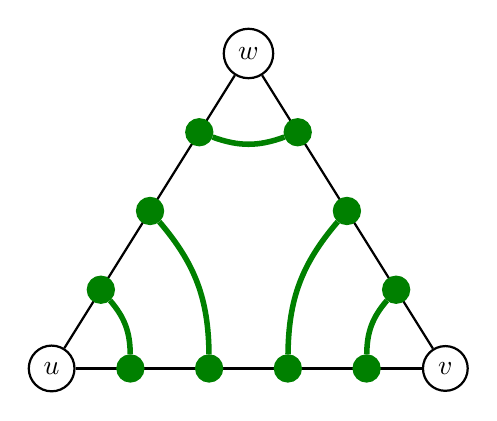
\begin{tikzpicture}[main/.style = {draw, circle, thick}, e/.style = {Green, bend right = 20, line width = 2pt}]
					\node[main] (u) at (0,0) {$u$};
					\node[main] (v) at (5,0) {$v$};
					\node[main] (w) at (2.5, 4) {$w$};
					\draw[thick] (u) -- (v);
					\draw[thick] (w) -- (v);
					\draw[thick] (u) -- (w);
					\node[main, fill, Green] (0) at (1,0) {};
					\node[main, fill, Green] (1) at (2,0) {};
					\node[main, fill, Green] (2) at (3,0) {};
					\node[main, fill, Green] (3) at (4,0) {};
					
					\node[main, fill, Green] (4) at (2.5/4,1) {};
					\node[main, fill, Green] (5) at (2.5/2,2) {};
					\node[main, fill, Green] (6) at (7.5/4,3) {};
					
					\node[main, fill, Green] (7) at (2.5 + 7.5/4,1) {};
					\node[main, fill, Green] (8) at (2.5 + 2.5/2,2) {};
					\node[main, fill, Green] (9) at (2.5 + 2.5/4,3) {};
					
					\draw[e] (0) edge (4);
					\draw[e] (1) edge (5);
					\draw[e] (7) edge (3);
					\draw[e] (8) edge (2);
					\draw[e] (6) edge (9);
				\end{tikzpicture}
				\caption{Example of connecting the triangle face edges.}
			\end{figure}
			
			\item Also we need to verify that this gives a correct curve $\gamma_e$, therefore no loops are present. For which we will use word equations $\mathcal{A} = \{\mathtt{a}, \mathtt{b}\}$. For every $f = \{u,v\} \in E_T$ we will introduce two variables $X_{uv}$ and $X_{vu}$ for which $l(X_{uv}) = l(X_{vu}) = c_{uv}(e)$. For every face $t = \{u,v,w\}$ and vertex $u \in t$ we will introduce variables $Y_{ut}$ and $Y_{tu}$, where $l(Y_{ut}) = l(Y_{tu}) = \frac{c_{xy} + c_{xz} - c_{xz}}{2}$. The equations will be as follows. For every $\{u,v\} = f \in E_T, f \in \partial \mathcal{S}$:
			
			$$
			X_{uv} = X_{vu} =
			\left\{
			\begin{array}{ll}
				\mathtt{b} & \text{if } f \text{ contains an endpoint of } \partial \mathcal{S}\\
				\emptyset & \text{otherwise}
			\end{array}
			\right.
			$$
			
			\noindent and for every face $t = \{u,v,w\}$ and edge $\{u,v\}$ we will have:
			
			$$
			X_{uv} = Y_{ut} Y_{tv}, X_{vu} = Y_{vt} Y_{tu}.
			$$
			
			\begin{observ}
				If $\gamma_e$ is a single connected curve, the system has a unique solution (all $\mathtt{b}$'s). Otherwise, there is a solution containing $\mathtt{a}$, we can find it efficiently.
			\end{observ}
		\end{itemize}
		\item Verify that for each $e_1,e_2 \in E, e_1 \neq e_2, \{e_1,e_2\} \notin R$ have $i (\gamma_{e_1}, \gamma_{e_1}) = 0$.
		
		\begin{itemize}
			\item Now we will denote $c_{uv} := c_{uv}(e_1) + c_{uv}(e_2)$ and then we will check that correctness as we did before.
			\item Next we also introduce similiar word equations. For alphabet $\mathcal{A} = \{\mathtt{a}, \mathtt{b}, \mathtt{c}\}$ and variables $X_{uv}, X_{vu},\\ Y_{ut}, Y_{tu}$ as was defined earlier. Only the length is different, for example $l(X_{uv}) = c_{uv} (e_1) + c_{vu}(e_2)$ and similarly for $l(Y_{ut}) = \dots$.
			
			For the first equations it will be more tricky since we can have both $e_1$ and $e_2$ intersecting $f \in E_T, f \subseteq \partial\mathcal{S}$. Otherwise it is straightforward how it is defined.
			
			For the next equations it will remain the same, which is $X_{uv} = Y_{ut} Y_{tv}, X_{vu} = Y_{vt} Y_{tu}$.
			
			\item Lastly we need to verify $X_{uv}$ has $c_{uv}(e_1)$ occurrences of $\mathtt{b}$ and also $c_{uv}(e_2)$ occurrences of $\mathtt{c}$.
		\end{itemize}
	\end{enumerate}
\end{proof}


By all these steps we have finished the proof that Weak AT-realization is in NP, because we only need to guess the numbers $c_{uv}(e)$ and add it to the NP algorithm, because with that we can in polynomial time check it is correct.

\begin{algorithm}[!ht]
	\begin{algorithmic}[1]
		\Require $G = (V,E), R \subseteq \binom{E}{2}$
		\State $\forall v \in V:$ choose $D_v$ (so that $v \neq w$ have $\overline{D_v} \cap \overline{D_w} = \emptyset$).
		\State For any edge $e \in E$ incident to $v \in V:$ choose an endpoint of $\gamma_e$ on $\partial D_v$.
		\State \textcolor{Green}{Create a triangulation $T$.}
		\State \textcolor{Green}{Guess all the numbers $c_{f}(e)$.}
	\end{algorithmic}
	\caption{NP algorithm for testing Weak AT-realization.}
\end{algorithm}
	\chapter{$\chi$-boundedness}

\begin{notation}
	$\chi(G) = $ chromatic number $G$ and $\omega(G) = $ is the maximal clique in $G$.
\end{notation}

\begin{observ}
	$\forall G: \chi(G) \geq \omega(G)$.
\end{observ}

\begin{defn}
	Graph class $\mathcal{C}$ is $\chi$-bounded if $\exists f : \N \to \N$ s.t. $\forall G \in \mathcal{C} : \chi(G) \leq f(\omega(G))$.
\end{defn}

\begin{example}
	$\chi$-omezené třídy: úplné grafy, rovinné grafy (funkce $f$ je konstantní), perfektní grafy.
\end{example}

\begin{observ}
	Intervalové, permutační, chordální, comparability, $\dots$ jsou perfektní a tudíž i $\chi$-omezené.
\end{observ}

\section{$\chi$-boundedness of CIRC graphs}

\begin{observ}
	Circular-Arc grafy splňují: $\chi(G) \leq 2 \omega(G)$.
\end{observ}

\begin{proof}
	Na kružnici máme intervaly. V jednom bodě kružnici rozstřihneme a obarvíme $\omega(G)$ barvami. Potom už máme jen intervalový graf, který je perfektní.
\end{proof}

\begin{defn}
	Následující definice jsou si ekvivalentní:
	
	\begin{itemize}
		\item $G \in \text{CIR}$.
		\item $G$ je průnikový graf sečen v kružnici.
		\item $G$ je průnikový graf půlkružnic nad $x$-ovou osou.
		\item $G$ se dá reprezentovat posloupností čísel, kde se každé číslo $1, \dots, n$ vyskytuje právě dvakrát a platí, že vrcholy $v_i, v_j$ spolu sousedí právě když ta posloupnost obsahuje podposloupnost $i,j,i,j$ nebo $j,i,j,i$.
	\end{itemize}
\end{defn}

\begin{thm}
	$\text{CIR}$ je $\chi$-omezená.
\end{thm}

\begin{notation}
	Pro $k \in \N$ definujeme $\text{CIR}(k) := \{G \in \text{CIR}: \omega (G) \leq k\}$.
\end{notation}

\begin{observ}
	$\text{CIR}(k) \subseteq \text{CIR}(k+1) \subseteq \dots \subseteq \text{CIR}$.
\end{observ}

Chceme dokázat, že $(\forall k \in \N) \ (\exists f(k) \in \N) \ : \forall G \in \text{CIR}(k)$ platí, že $\chi(G) \leq f(k)$.

\begin{defn}
	Mějme $G \in \text{CIR}$ reprezentovaný jako průnikový graf půlkružnic. Pro $p,q \in \N_0$ $(p,q)$\textbf{-konfigurace} je množina $p+q$ vrcholů $x_1, \dots, x_p, y_1, \dots, y_q$ takové, že půlkružnice mají tuto vzájemnou polohu zobrazenou na obrázku \ref{konf}.
	
	\begin{figure}[!ht]\centering
		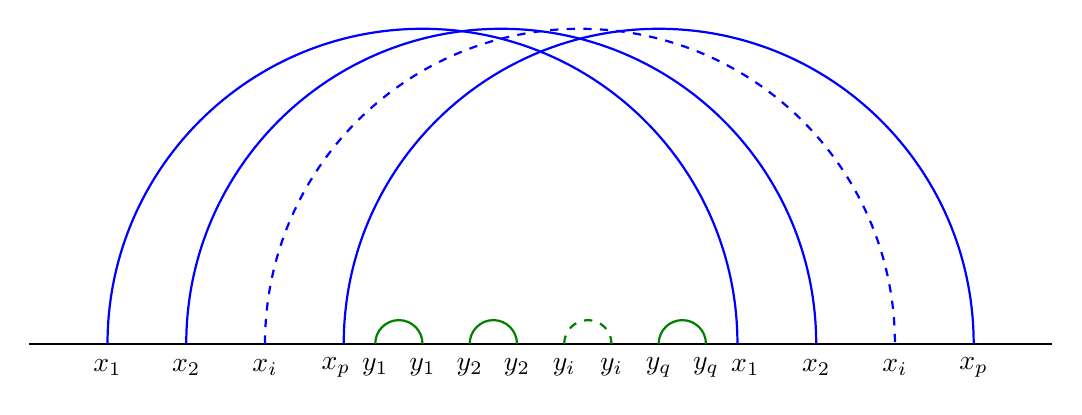
\begin{tikzpicture}
			\draw[thick] (0,0) -- (13,0);
			\draw[color=Blue, thick] (1,0) arc (180:0:4);
			\draw[color=Blue, thick] (2,0) arc (180:0:4);
			\draw[color=Blue, thick, dashed] (3,0) arc (180:0:4);
			\draw[color=Blue, thick] (4,0) arc (180:0:4);
			\draw[color=Green, thick] (4.4,0) arc (180:0:.3);
			\draw[color=Green, thick] (5.6,0) arc (180:0:.3);
			\draw[color=Green, thick, dashed] (6.8,0) arc (180:0:.3);
			\draw[color=Green, thick] (8,0) arc (180:0:.3);
			\node at (1, -.3) {$x_1$};
			\node at (2, -.3) {$x_2$};
			\node at (3, -.3) {$x_i$};
			\node at (3.9, -.3) {$x_p$};
			\node at (4.4, -.3) {$y_1$};
			\node at (5, -.3) {$y_1$};
			\node at (5.6, -.3) {$y_2$};
			\node at (6.2, -.3) {$y_2$};
			\node at (6.8, -.3) {$y_i$};
			\node at (7.4, -.3) {$y_i$};
			\node at (8, -.3) {$y_q$};
			\node at (8.6, -.3) {$y_q$};
			\node at (9.1, -.3) {$x_1$};
			\node at (10, -.3) {$x_2$};
			\node at (11, -.3) {$x_i$};
			\node at (12, -.3) {$x_p$};
		\end{tikzpicture}
		\caption{Definice $(p-q)$-konfigurace.}
		\label{konf}
	\end{figure}
\end{defn}

\begin{notation}
	$\text{CIR}(k,p,q) = \{G \in \text{CIR}, \omega(G) \leq k, G \text{ má reprezentaci bez } (p,q)\text{-konfigurace}\}$.
\end{notation}

\begin{observ}
	Pro $p > k$ a libovolné $q \in \N_0$: $\text{CIR}(k,p,q) = \text{CIR}(k)$.
\end{observ}

\begin{claim}
	$\forall k \in \N \ \forall p, q \in \N_0 \ \exists g(k,p,q) \in \N$ t.ž. $\forall G \in \text{CIR}(k,p,q) : \chi(G) \leq g(k,p,q)$.
\end{claim}

\begin{observ}
	Důkazem tohoto tvrzení platí věta.
\end{observ}

\begin{proof}
	Dané tvrzení dokážeme pomocí dvojité indukce: Indukcí podle $p \in \N_0$:
	
	\begin{lemma}
		$\forall G \in \text{CIR}(k,0,q) : \chi (G) \leq k (q-1)$ pro $q \geq 2$.
	\end{lemma}
	
	\begin{proof}[Proof of lemma]
		Indukcí podle $q \in \N_0$. Pokud $q = 2$ tak můžeme pozorovat, že všechny obloučky protínají společnou souvislou přímku. Tím pádem $\forall k : \text{CIR}(k,0,2) \subseteq \text{PER}$ které jsou perfektní.
		
		Nyní nechť $q > 2$. Nechť $G \in \text{CIR}(k, 0, q)$, vrcholy $G$ rozdělíme na 2 části $V_1, V_2$ tak, že
		
		\begin{itemize}
			\item $V_1$ bude indukovat graf z $\text{CIR}(k,0,2)$ a
			\item $V_2$ bude indukovat graf z $\text{CIR}(k,0,q-1)$.
		\end{itemize}
		
		Označme $\pi$ jakožto nejpravější levý konec obloučku. Potom $V_1$ jsou vrcholy, které mají levý konec vlevo od $\pi$. A $V_2$ jsou vrcholy, které mají levý konec napravo od $\pi$. Pak už použijeme indukci.
	\end{proof}
	
	\begin{lemma}
		Nechť $p \geq 1, q \geq 1$. Potom $\forall G \in \text{CIR}(k,p,q):$ vrcholy $G$ lze rozdělit na 2 části $V_A, V_B$ tak, že každá komponenta $G[V_A]$ i $G[V_B]$ patří do $\text{CIR}(k, p-1, 2q+1)$.
	\end{lemma}
	
	\begin{cor}
		Lze vzít $g(k,p,q) = g (k, p-1, 2q+1)$ tedy tvrzení pak platí.
	\end{cor}
	
	\begin{proof}[Proof of lemma]
		Mějme $G \in \text{CIR}(k,p,q)$. BÚNO: $G$ je souvislý a máme danou reprezentaci. Nechť $x_0$ je vrchol $G$ jehož oblouček má nejlevější levý konec. Definujeme $V_i := \{x \in V(G) : \text{ nejkratší cesta v } G \text{ od } x_0 \text{ do } x$ má délku $i\}$.
		
		\begin{observ}
			Pokud vede hrana z $V_i$ do $V_j$ tak $|i - j| \leq 1$.
		\end{observ}
		
		\begin{observ}
			Z každého vrcholu $V_{i+1}$ vede aspoň 1 hrana do $V_i$.
		\end{observ}
		
		Nyní tvrdíme, že žádná komponenta $G[V_i]$ neobsahuje $(p-1, 2q + 1)$-konfiguraci.
		
		Nechť $C$ je komponenta $G[V_i]$ pro spor obsahující $(p-1, 2q + 1)$-konfiguraci. Označme $y_{q+1}$ nějaký oblouček $w$ musí protnout $y_{q+1}$, tedy $w \in V_{i-1}$. Aspoň jeden konec je mimo $C$. $V_{i-1} = V_0$ tedy hotovo. Kdyby měl oba konce v $C$, tak nelze protnout oblouček z $V_{i-2}$.
		
		Nyní nechť $x_1, \dots, x_{p-1}, y_{1}, \dots, y_{2q+1}$ je $(p-1, 2q + 1)$-konfigurace. Nechť $I$ je interval mezi nejlevějším a nejpravějším koncem obloučku v $C$.
		
		\begin{observ}
			Každý soused $w \in V_{i-1}$ vrcholu $y_{q+1}$ musí mít jeden konec mimo $I$.
		\end{observ}
		
		Potom $w, x_1, \dots, x_{p-1}, y_{1}, \dots, y_q$ nebo $w, x_1, \dots, x_{p-1}, y_{q+2}, \dots, y_{2q+1}$ je $(p,q)$-konfigurace v $G$, což je spor.
		
		Závěrem $V_{A} := \cup_{i \text{ sudé}} V_{i}$ a $V_{B} := \cup_{i \text{ liché}} V_{i}$.
	\end{proof}
\end{proof}

\section{$\chi$-unboundedness of SEG graphs}

\begin{defn}
	SEG is the class of graphs of intersection graphs of segments in the plane.
\end{defn}

Now the question might be if SEG graphs are $\chi$-bounded or not. This was firstly stated by Erdös. The answer came later by the following theorem.

\begin{thm}[Pawlik, Kozik, Krawczyk, Lagos, Micek, Trotter, Wolezak, 2012]
	$\forall k \in \N$ there exists triangle-free graph $G_k \in \text{SEG}$ with $\chi(G_k) \geq k$.
	\label{PKKLMTW thm}
\end{thm}

\begin{defn}
	\textbf{L-curve} is a union of a horizontal and vertical segment sharing a common bottom-left endpoint. \textbf{L-graph} is an intersection graph of L-curves.
\end{defn}

\begin{thm}
	Any L-graph is also SEG-graph.
\end{thm}

\begin{proof}
	Suppose $\mathcal{L} = \{l_1, l_2, \dots, l_n\}$ is a set of L-curves, we will show by induction on $\abs{\mathcal{L}} = n$ that there is a set $\mathcal{S} = \{s_1, s_2, \dots, s_n\}$ of segments s.t. $l_i \cap l_j \neq \emptyset \Leftrightarrow s_i \cap s_j \neq \emptyset$, and moreover:
	
	\begin{enumerate}
		\item all $s_1, \dots, s_n$ lie in the half plane below the $x$-axis;
		\item $s_i$ touches the $x$-axis \ifft $l_i$ can be extended upwards to infinity without crossing any other $l_j \in \mathcal{L}$;
		\item left-to-right order of $s_i$'s touching the $x$-axis is the same as for $l_i$'s.
	\end{enumerate}
	
	Now for $n = 1$ it is simple, see Fig. \ref{start-l-curves}, and for $n > 1$ \wlogt $l_n$ has topmost horizontal part. By induction we represent $\mathcal{L}' = \{l_1, \dots, l_{n-1}\}$ by $\mathcal{S}' = \{s_1, \dots, s_{n-1}\}$ then
	
	\begin{enumerate}
		\item shorten the $s_i$ if $l_i$ no longer can extend upwards and
		\item insert $s_n$ touching $x$-axis, nearly horizontal. See Fig. \ref{induction-l-curves}.
	\end{enumerate}
	
	\begin{figure}[!ht]\centering
		\begin{subfigure}{.45\textwidth}\centering
			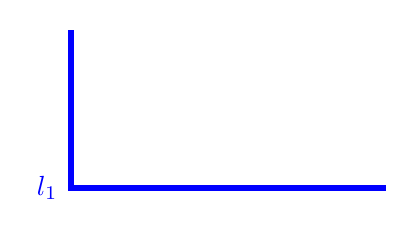
\begin{tikzpicture}[l/.style = {line width = 2pt}, b/.style = {Blue}]
				\draw[l, b] (0,2) to[out=270, in=90] (0,0) to[out=0, in=180] (4,0);
				\node[b] at (-.3,0) {$l_1$};
			\end{tikzpicture}
			\caption{L-curves.}
		\end{subfigure}
		\begin{subfigure}{.45\textwidth}\centering
			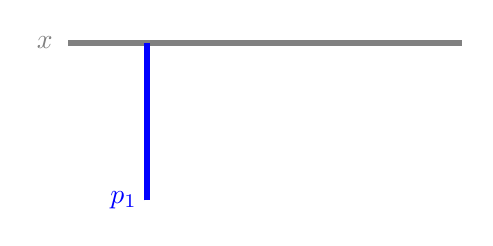
\begin{tikzpicture}[l/.style = {line width = 2pt}, b/.style = {Blue}]
				\draw[l, gray] (0,0) -- (5,0);
				\node[gray] at (-.3,0) {$x$};
				\draw[l, b] (1, -2) -- (1,0);
				\node[b] at (.7, -2) {$p_1$};
			\end{tikzpicture}
			\caption{Segments.}
		\end{subfigure}
		\caption{Simple of start for an induction.}
		\label{start-l-curves}
	\end{figure}
	
	\begin{figure}[!ht]\centering
		\begin{subfigure}{.45\textwidth}\centering
			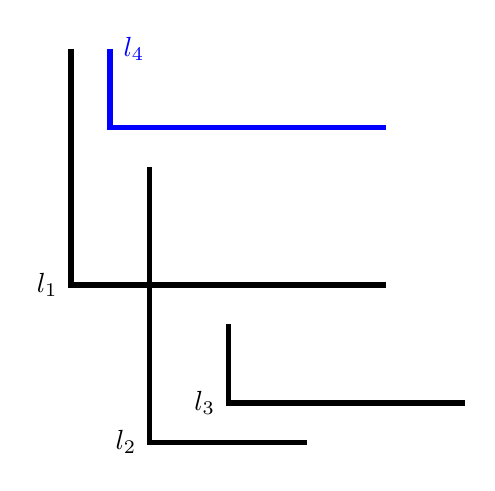
\begin{tikzpicture}[l/.style = {line width = 2pt}]
				\draw[l] (0,3) to[out=270, in=90] (0,0) to[out=0, in=180] (4,0);
				\node at (-.3,0) {$l_1$};
				\draw[l] (1,1.5) to[out=270, in=90] (1,-2) to[out=0, in=180] (3,-2);
				\node at (.7,-2) {$l_2$};
				\draw[l] (2,-.5) to[out=270, in=90] (2,-1.5) to[out=0, in=180] (5,-1.5);
				\node at (1.7,-1.5) {$l_3$};
				\draw[l, Blue] (.5,3) to[out=270, in=90] (.5,2) to[out=0, in=180] (4,2);
				\node[Blue] at (.8,3) {$l_4$};
			\end{tikzpicture}
			\caption{L-curves.}
		\end{subfigure}
		\begin{subfigure}{.45\textwidth}\centering
			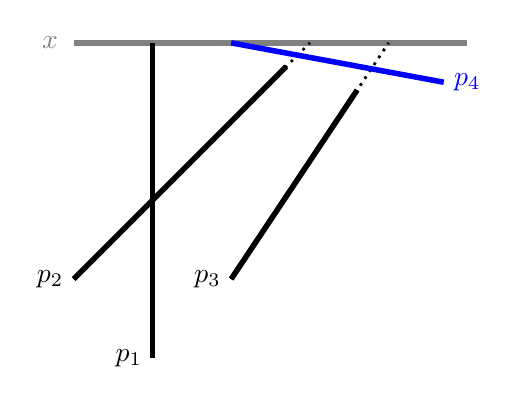
\begin{tikzpicture}[l/.style = {line width = 2pt}]
				\draw[l, gray] (0,0) -- (5,0);
				\node[gray] at (-.3,0) {$x$};
				\draw[l] (1, -4) -- (1,0);
				\node at (.7, -4) {$p_1$};
				\draw[l] (0, -3) -- (2.7,-.3);
				\draw[dotted, line width = 1pt] (0, -3) -- (3,0);
				\node at (-.3, -3) {$p_2$};
				\draw[l] (2, -3) -- (3.6,-.6);
				\draw[dotted, line width = 1pt] (2, -3) -- (4,0);
				\node at (1.7, -3) {$p_3$};
				\draw[l, Blue] (4.7, -.5) -- (2,0);
				\node[Blue] at (5, -.5) {$p_4$};
			\end{tikzpicture}
			\caption{Segments.}
		\end{subfigure}
		\caption{Simple example for conversion.}
		\label{induction-l-curves}
	\end{figure}
\end{proof}

\begin{proof}[Proof of theorem \ref{PKKLMTW thm}]
	In fact we show that $\forall k \in \N$ there exists triangle-free L-graph $G_k$ with $\chi(G_k) \geq k$.
	
	\begin{defn}
		A \textit{configuration} is
		
		\begin{enumerate}
			\item a collection of L-curves inside the unit square $[0,1] \times [0,1]$, whose intersection graph is triangle-free;
			\item a set $\{P_1, \dots, P_m\}$ of \textit{"probes"} which are pairwise disjoint rectangles inside $[0,1] \times [0,1]$ touching its bottom boundary;
			\item any L-shape from the collection intersecting a probe $P_i$ must cross it from left to right; \label{conf-3}
			\item the L-shape crossing a given probe are pairwise disjoint. \label{conf-4}
		\end{enumerate}
		
		\begin{figure}[!ht]\centering
			\begin{subfigure}{.45\textwidth}\centering
				\begin{tikzpicture}[l/.style = {line width = 1pt}]
					\draw[Blue, fill=Blue!20] (0,0) rectangle (6,6);
					\draw[Red, fill=Red!20] (1,0) rectangle (2,4);
					\draw[Red, fill=Red!20] (3,0) rectangle (5,3);
					\draw[l] (.5,5) to[out=270, in=90] (.5,1) to[out=0, in=180] (2.5,1);
					\draw[l] (2.3,2) to[out=270, in=90] (2.3,1.5) to[out=0, in=180] (5.4,1.5);
					\draw[l] (2.6,3) to[out=270, in=90] (2.6,2) to[out=0, in=180] (5.6,2);
					\draw[l] (3,5.5) to[out=270, in=90] (3,4) to[out=0, in=180] (5,4);
				\end{tikzpicture}
				\caption{Example of configuration where we have \textcolor{Red}{two probes} in a \textcolor{Blue}{[0,1] box} with four L-curves.}
			\end{subfigure}
			\begin{subfigure}{.45\textwidth}\centering
				\begin{tikzpicture}[l/.style = {line width = 1pt}]
					\draw[Blue, fill=Blue!20] (0,0) rectangle (6,6);
					\draw[Red, fill=Red!20] (1,0) rectangle (2,4);
					\draw[Red, fill=Red!20] (3,0) rectangle (5,3);
					\draw[l] (2.6,2) to[out=270, in=90] (2.6,.5) to[out=0, in=180] (4.6,.5);
					\draw[l] (4,4) to[out=270, in=90] (4,2) to[out=0, in=180] (4.6,2);
					\draw[l] (.5,5) to[out=270, in=90] (.5,1) to[out=0, in=180] (2.5,1);
					\draw[l] (.7,5) to[out=270, in=90] (.7,.5) to[out=0, in=180] (2.5,.5);
				\end{tikzpicture}
				\caption{Counterexample of violating the definitions \ref{conf-3} and \ref{conf-4}.}
			\end{subfigure}
			\caption{Example and counterexamples of the definition.}
		\end{figure}
	\end{defn}
	
	We will construct two sequences of $A_1, A_2, A_3, \dots$ and $B_1, B_2, B_3, \dots$ of configurations s.t.:
	
	\begin{enumerate}
		\item $\forall k \in \N$ in any proper coloring of the L-curves in $A_k$, the L-curves seen inside the probes use at least $k$ different colors.
		\item $\forall k \in \N$ in any proper coloring of the L-curves in $B_k$ there exist a probe of $B_k$ which is crossed by L-curves of at least $k$ different colors.
	\end{enumerate}
	
	By induction for $k = 1$ it is straightforward, see Fig. \ref{start-configuration}. Now we show two parts.
	
	\begin{figure}[!ht]\centering
		\begin{tikzpicture}[l/.style = {line width = 1pt}]
			\draw[Blue, fill=Blue!20] (0,0) rectangle (3,3);
			\draw[Red, fill=Red!20] (1,0) rectangle (2,2);
			\draw[l] (.5,2.6) to[out=270, in=90] (.5,1) to[out=0, in=180] (2.5,1);
		\end{tikzpicture}
		\caption{Start of the induction with \textcolor{Red}{one probe} and one L-curve.}
		\label{start-configuration}
	\end{figure}
	
	\begin{enumerate}
		\item From $B_k$ to $A_k+1$. See Fig. \ref{ak+1}.
		\begin{enumerate}
			\item Insert one new L-shape inside every probe of $B_k$ and
			\item replace each probe by 2 new probes.
		\end{enumerate}
		\item From $B_k$ and $A_{k+1}$ to $B_{k+1}$. See Fig. \ref{bk+1}.
		\begin{enumerate}
			\item Insert a small copy of $A_{k+1}$ near the top of every probe of $B_k$ and
			\item extend the probes of these small copies all the way down to obtain probes of $B_{k+1}$.
		\end{enumerate}
	\end{enumerate}
	
	\begin{figure}[!ht]\centering
		\begin{subfigure}{.45\textwidth}\centering
			\begin{tikzpicture}[l/.style = {line width = 1pt}]
				\draw[Blue, fill=Blue!20] (0,0) rectangle (6,6);
				\draw[Red, fill=Red!20] (1,0) rectangle (2,4);
				\draw[Red, fill=Red!20] (3,0) rectangle (5,3);
				\draw[l] (1,1) to (2,1);
				\draw[l] (1,2) to (2,2);
				\draw[l] (1,3) to (2,3);
				\draw[l] (3,1) to (5,1);
				\draw[l] (3,2) to (5,2);
				\node at (5,5) {$B_k$};
			\end{tikzpicture}
			\caption{Simplification with \textcolor{Red}{two probes}.}
		\end{subfigure}
		\begin{subfigure}{.45\textwidth}\centering
			\begin{tikzpicture}[l/.style = {line width = 1pt}]
				\draw[Blue, fill=Blue!20] (0,0) rectangle (6,6);
				\draw[Red, fill=Red!20] (1,0) rectangle (2,4);
				\draw[Red, fill=Red!20] (3,0) rectangle (5,3);
				\draw[VioletRed, fill=VioletRed!20] (1.1,0) rectangle (1.2,3.7);
				\draw[VioletRed, fill=VioletRed!20] (1.4,0) rectangle (1.6,.8);
				\draw[l] (1,1) to (2,1);
				\draw[l] (1,2) to (2,2);
				\draw[l] (1,3) to (2,3);
				\draw[l, Green] (1.3,3.6) to[out=270, in=90] (1.3,.5) to[out=0, in=180] (1.7,.5);
				\draw[VioletRed, fill=VioletRed!20] (3.1,0) rectangle (3.4,2.7);
				\draw[VioletRed, fill=VioletRed!20] (3.6,0) rectangle (4.4,.8);
				\draw[l] (3,1) to (5,1);
				\draw[l] (3,2) to (5,2);
				\draw[l, Green] (3.5,2.6) to[out=270, in=90] (3.5,.5) to[out=0, in=180] (4.5,.5);
				\node at (4.3,5) {$B_k \to A_{k+1}$};
			\end{tikzpicture}
			\caption{\textcolor{Green}{Two new L-curves} and \textcolor{VioletRed}{four new probes}.}
		\end{subfigure}
		\caption{Conversion from $B_k$ to $A_{k+1}$.}
		\label{ak+1}
	\end{figure}
	
	\begin{figure}[!ht]\centering
		\begin{subfigure}{.45\textwidth}\centering
			\begin{tikzpicture}[l/.style = {line width = 1pt}]
				\draw[Blue, fill=Blue!20] (0,0) rectangle (6,6);
				\draw[Red, fill=Red!20] (1,0) rectangle (2,4);
				\draw[Red, fill=Red!20] (3,0) rectangle (5,3);
				\draw[l] (1,1) to (2,1);
				\draw[l] (1,2) to (2,2);
				\draw[l] (1,3) to (2,3);
				\draw[l] (3,1) to (5,1);
				\draw[l] (3,2) to (5,2);
				\node at (5,5) {$B_k$};
			\end{tikzpicture}
			\caption{Simplification with \textcolor{Red}{two probes}.}
		\end{subfigure}
		\begin{subfigure}{.45\textwidth}\centering
			\begin{tikzpicture}[l/.style = {line width = 1pt}]
				\draw[Blue, fill=Blue!20] (0,0) rectangle (6,6);
				\draw[Red, fill=Red!20] (1,0) rectangle (2,4);
				\draw[Red, fill=Red!20] (3,0) rectangle (5,3);
				\draw[Violet, fill=Violet!20] (1.1, 3.1) rectangle (1.9, 3.9);
				\draw[VioletRed, fill=VioletRed!20] (1.2, 0) rectangle (1.6, 3.6);
				\draw[Violet, fill=Violet!20] (3.6, 2.1) rectangle (4.4, 2.9);
				\draw[VioletRed, fill=VioletRed!20] (3.7, 0) rectangle (4.1, 2.6);
				\draw[l] (1,1) to (2,1);
				\draw[l] (1,2) to (2,2);
				\draw[l] (1,3) to (2,3);
				\draw[l] (3,1) to (5,1);
				\draw[l] (3,2) to (5,2);
				\node at (4,5) {$B_k \ \& \ A_{k+1} \to B_{k+1}$};
			\end{tikzpicture}
			\caption{\textcolor{Violet}{Copies of $A_{k+1}$} and \textcolor{VioletRed}{prolonged probes}.}
		\end{subfigure}
		\caption{Conversion from $A_{k+1}$ and $B_{k}$ to $B_{k+1}$.}
		\label{bk+1}
	\end{figure}
\end{proof}

Now we may ask ourselves if this prove can be extended to some other type of intersection graphs. Well indeed it can be done. Note that \textit{arc-connected} set means that all pairs from the set can be connected via an arc.

\begin{fact}
	For any compact arc-connected set $X \subseteq \R^2$ other then an axis parallel rectangle there is a triangle-free graph $G_k$, $\chi(G_k) \geq k$, which is the intersection graph of horizontally and vertically scaled copies of $X$.
\end{fact}

\begin{defn}
	A graph $G$ is $d$-degenerate if every non-empty subgraph of $G$ contains a vertex of degree at most $d$.
\end{defn}

\begin{observ}
	$G$ is $d$-degenerate then $\chi(G) \leq d+1$.
\end{observ}

\begin{proof}
	This observation can be seen by induction. Lets take $u$ which has $\deg(u) \leq d$ now take $G - u$ which is also $d$-degenerate and therefore by induction hypothesis colorable by $d+1$ colors. Lets take such coloring and now give $u$ a possible color. Because it only has $d$ neighbors we will have at least 1 possibility.
\end{proof}

\section{Axis-parallel rectangles intersection graphs}

\begin{thm}[Asblund, Grunbaum]
	If $G$ is an intersection graph of axis parallel rectangles in the plane then $\chi(G) \leq O(\omega^2 (G))$.
\end{thm}

\begin{proof}
	Suppose we have $G = (V,E)$ as above: each vertex $u \in V$ is represented by a rectangle $R_u$. Let $E = E_1 \dot{\cup} E_2$ as follows
	
	\begin{enumerate}
		\item $\{u,v\} \in E_1$ if a vertex of $R_u$ is inside $R_v$ or vice versa (Fig. \ref{inter-box})
		\item $E_2 = E \setminus E_1$ if it is cross-like (Fig. \ref{cross-box}).
	\end{enumerate}
	
	\begin{figure}[!ht]\centering
		\begin{subfigure}{.45\textwidth}\centering
			\begin{tikzpicture}
				\draw[VioletRed, fill=VioletRed!20] (0, 0) rectangle (2, 2);
				\draw[VioletRed, fill=VioletRed!20, opacity=0.8] (1, 1) rectangle (3, 3);
			\end{tikzpicture}
			\caption{One vertex is inside the other rectangle.}
			\label{inter-box}
		\end{subfigure}
		\begin{subfigure}{.45\textwidth}\centering
			\begin{tikzpicture}
				\draw[VioletRed, fill=VioletRed!20] (0, 1) rectangle (3, 2);
				\draw[VioletRed, fill=VioletRed!20, opacity=0.8] (1, 0) rectangle (2, 3);
			\end{tikzpicture}
			\caption{Cross-like intersection.}
			\label{cross-box}
		\end{subfigure}
		\caption{Two possibilities.}
	\end{figure}
	
	Lets denote $G_1 = (V, E_1)$, $G_2 = (V, E_2)$ and $k = \omega(G)$. We will show $\chi(G_1) = O(k)$ and $\chi(G_2) = O(k)$.
	
	\begin{itemize}
		\item For $G_1$ we claim that $|E_1| \leq 4 k \cdot |V|$ (and any subgraph of $G_1$ induced by $W \subseteq V$ has at most $4 k \cdot |W|$ edges). This is because each vertex of a rectangle is inside at most $k-1$ other rectangles, due to the maximal clique. So this means one for each vertex of a rectangle is in total $4 (k-1)$. Now we direct an edge $uv$ if vertex of $R_u$ is inside $R_v$. Thus the outdegree of any vertex is $\leq 4 (k-1)$ so $|E_1| \leq 4 (k-1) \cdot |V|$. Hence $G_1$ (and any of its induced subgraphs) has average degree $\frac{2 |E_1|}{|V|} = 8 (k-1)$. So the min degree is $\leq 8 (k-1)$ therefore it is $8(k-1)$-degenerate and hence $\chi(G_1) \leq 8 (k-1) + 1$.
		\item For $G_2$ we claim that $\chi(G_2) = \omega(G_2) = O(k)$ because $G_2$ is a comparability graph (for example sort the boxes from tallest to shortest).
		\item For $G$ we have $\chi(G) \leq \chi(G_1) \cdot \chi(G_2) = O(k^2)$. For this lets have $E_1 \dot{\cup} E_2$ and see Fig. \ref{two-colors}. That is we have coloring $1,2, \dots, p$ colors for $E_1$ and $1,2, \dots, q$ colors for $E_2$ and we create a coloring by tuples $(x,y)$ where $x \in [p]$ and $y \in [q]$.
	\end{itemize}
	
	\begin{figure}[!ht]\centering
		\begin{tikzpicture}[node distance = 30mm, main/.style = {draw, circle, thick}]
			\node[main] (0) {(1,\textcolor{Green}{1})};
			\node[main, above of = 0] (1) {(2,\textcolor{Green}{1})};
			\node[main, left of = 1] (2) {(3,\textcolor{Green}{1})};
			\node[main, right of = 1] (3) {(2,\textcolor{Green}{2})};
			\node[main, left of = 0] (4) {(1,\textcolor{Green}{3})};
			\node[main, above of = 2] (5) {(1,\textcolor{Green}{3})};
			\draw[thick] (0) -- (1);
			\draw[thick] (0) -- (2);
			\draw[thick] (1) -- (2);
			\draw[thick] (1) -- (5);
			\draw[thick, Green] (0) -- (3);
			\draw[thick, Green] (0) -- (5);
			\draw[thick, Green] (1) -- (4);
			\draw[thick, Green] (1) -- (3);
			\draw[thick, Green] (2) -- (4);
			\draw[thick, Green] (2) -- (5);
			\draw[thick, Green] (3) -- (4);
			\draw[thick] (3) -- (5);
		\end{tikzpicture}
		\caption{Disjoint union of edges for coloring.}
		\label{two-colors}
	\end{figure}
\end{proof}

\section{1-String with big girth}

Now we will continue further and see that L-graphs $\subseteq$ (proper, i.e. not overlapping segments) SEG $\subseteq$ 1-String $\subseteq$ String. For this we need to see the definitions first.

\begin{defn}
	$G \in$ 1-String if $G$ has a String representation in which every two strings intersect at most once.
\end{defn}

\begin{defn}
	The \textbf{girth} of a graph $G$ is the length of the shortest cycle in $G$, if $G$ has no cycle then girth is $+ \infty$. We will denote girth of $G$ as $\gamma(G)$.
\end{defn}

With the newly established terminology we have previously shown that L-graphs of girth $\geq 4$ have unbounded $\chi$, but what about girth $\geq 5$ (or $6, \dots$). Also we will give a remark which is that for arbitrary large girth and chromatic number can be created. This can be shown by probabilistic techniques.

\begin{thm}[Kostochka \& Nešetřil]
	Let $G$ be a 1-String graph, then
	$$
	\begin{array}{r c l r}
		\text{if } \gamma(G) \geq 5 & \Rightarrow & \chi(G) \leq 6 & (\text{degeneracy } \leq 5), \\
		\text{if } \gamma(G) \geq 6 & \Rightarrow & \chi(G) \leq 4 & (\text{degeneracy } \leq 3), \\
		\text{if } \gamma(G) \geq 8 & \Rightarrow & \chi(G) \leq 3 & (\text{degeneracy } \leq 2). \\
	\end{array}
	$$
\end{thm}

\begin{proof}
	Let $G = (V,E)$ be a connected 1-String graph, with a given 1-String representation. $n = |V|, m = |E|$. We will show the minimal degree of this graph where the degeneracy will follow, since its subgraphs can only have larger girth. Let $H = (V_H, E_H)$ be a plane graph whose drawing is obtained by placing a vertex on every crossing of strings of $G$, pieces of string between adjacent crossings are the edges of $H$. Recall Euler's formula $v - e + f = 2 \geq 0$.
	
	$$
	\begin{aligned}
		&v = |V_H| = \frac{1}{2} \sum_{v \in V} \deg(v) = m \\
		&e = |E_H| = \sum_{w \in V}(\deg(w) - 1) = \left(\sum_{w \in V} \deg (w)\right) - n = 2m - n \\
		&f = \text{\# of faces of } H
	\end{aligned}
	$$
	
	\begin{observ}
		If $H$ has a face bounded by a cycle of length $l$, then $G$ has a closed walk of length $l$ in which each edge appears at most once. Hence $\gamma(G) \leq l$.
	\end{observ}
	
	And consequently every face of $H$ is incident to at least $\gamma(G)$ edges of $H$. Hence $f \cdot \gamma(G) \leq 2 e$.
	
	$$
	f \leq \frac{2e}{\gamma(G)} = \frac{4m - 2n}{\gamma(G)}
	$$
	
	So we can use the following computation.
	
	$$
	0 < v - e + f \leq m - 2m + n + \frac{4m - 2n}{\gamma(G)} = n \left(1 - \frac{2}{\gamma(G)} \right) - m \left(1 - \frac{4}{\gamma(G)} \right)
	$$
	
	\noindent This enforces the following.
	
	$$
	m \left(1 - \frac{4}{\gamma(G)}\right) < n \left(1 - \frac{2}{\gamma(G)} \right)
	$$
	
	\noindent Thus the min. degree $\leq$ average degree which is
	
	$$
	= \frac{2m}{n} \leq \frac{2 \left(1 - \frac{2}{\gamma(G)} \right)}{\left(1 - \frac{4}{\gamma(G)}\right)} = \frac{2 (\gamma(G) -2)}{\gamma(G) - 4}
	$$
	
	\noindent Lastly we compute the exact values. If $\gamma(G) \geq 5$ then min degree $< 6$ so $\leq 5$ hence $\chi(G) \leq 6$. If $\gamma(G) \geq 6$ then min degree $< 4$ so $\leq 3$ hence $\chi(G) \leq 4$. If $\gamma(G) \geq 8$ then min degree $< 3$ so $\leq 2$ hence $\chi(G) \leq 3$.
\end{proof}

Now we will further generalize to String graphs, which will use completely new topic which is called Game of robber and cops. Note that there exists more versions of this game.

\section{Game of robber and cops}

We have a given graph $G$. Then 1 robber (\textcolor{Red}{\faCircle}) and $c$ cops (\textcolor{Green}{\faSquare}). This game is for 2 players. Both players take turns. First one plays with cops and the second with robber.

\begin{mybox}{Rules}
	\begin{itemize}[]
		\item \textbf{Start of the game:} First player places cops on vertices of graph $G$. Then second player places the robber on some vertex.
		\item \textbf{Single turn:} First player can with each cop either move to adjacent vertex or stay in the same one. Then the robber can move to adjacent or stay in the same vertex.
		\item \textbf{Goal:} If both cop and robber end up in the same vertex cops have won. Alternatively robber wants to stay as long as possible.
	\end{itemize}
\end{mybox}

\begin{example}
	We have an easy example of the given graph and robber and cops. See Fig. \ref{cops-robber}
	
	\begin{figure}[!ht]\centering
		\begin{tikzpicture}[node distance = 15mm, main/.style = {draw, circle}, thick]
			\node[main] (0) {\textcolor{Green}{\faSquare}};
			\node[main, below of = 0] (1) {\textcolor{Green}{\faSquare}};
			\node[main, left of =1] (2) {};
			\node[main, right of =1] (3) {};
			\node[main, below of =1] (4) {};
			\node[main, left of=4] (5) {\textcolor{Green}{\faSquare} \textcolor{Green}{\faSquare}};
			\node[main, right of=4] (6) {\textcolor{Red}{\faCircle}};
			\node[main, below of =6] (7) {};
			\draw (0) -- (1);
			\draw (1) -- (2);
			\draw (0) -- (2);
			\draw (1) -- (3);
			\draw (0) -- (3);
			\draw (1) -- (4);
			\draw (2) -- (4);
			\draw (3) -- (4);
			\draw (5) -- (4);
			\draw (6) -- (4);
			\draw (7) -- (4);
			\draw (7) -- (6);
			\draw (2) -- (5);
		\end{tikzpicture}
		\caption{Example for cops and robber game.}
		\label{cops-robber}
	\end{figure}
\end{example}



\begin{defn}
	The \textbf{cop-number} $\cn(G) :=$ smallest number of cops for which the cops have a winning strategy on $G$. And for class $\mathcal{C}$ of graphs we define $\cn(\mathcal{C}) := \sup \{\cn (G), G \in \mathcal{C}, G \text{ connected}\}$.
\end{defn}

\begin{example}[Cycles]
	For cycles $C_n$ with $n \geq 4$ we can easily see that $\cn(G) = 2$ because we may put two cops in one vertex and then enclose the circle by two pats. Alternatively one is not enough since the robber may only wait and if cop is in the neighboring vertex the robber moves away.
\end{example}

\begin{example}[Int]
	In Int which is class of interval graphs we may find out that $\cn(\text{Int}) = 1$. Firstly we sort the intervals by its left endpoints, then place cop in the leftmost interval. The strategy is either catch a robber or move right to the next interval. If robber could move away the robber must stay way apart to the right or left. But note that if he would be in the left we didn't follow our strategy.
	
	Alternatively we can say the Int has a clique-path decomposition and in each step we are either in the same clique so we can catch the robber or we may move to the next clique.
\end{example}

\begin{prop}
	Let $G$ be a graph with $\gamma(G) \geq 5$. If every vertex of $G$ has degree $\geq d$, then $\cn(G) \geq d$.
	\label{girth-cop}
\end{prop}

\begin{proof}
	If $v$ is the robbers current vertex and $v_1, v_2, \dots, v_k$ are the neighbours of $v$, then each cop can be in the closed neighbourhood of at most one of $v_1, v_2, \dots, v_k$. If $k > \#$ of cops, robber may move to a "safe" neighbour $v_i$ if needed.
\end{proof}

\begin{cons}
	If $\mathcal{C}$ is a class of graphs closed under induced subgraphs with $\cn(\mathcal{C}) = c < + \infty$, then every graph $G \in \mathcal{C}$ of girth $\geq 5$ is $c$-degenrate and hence $\chi(G) \leq c+1$.
\end{cons}

\begin{thm}[Das and Gahlawat, 2022]
	$\cn(\text{String}) \leq 13$.
\end{thm}

We won't show this theorem. Also the lower bound is known to be 3. Also String graphs of girth $\geq 5$ have $\chi \leq 14$ which follows from the theorem and proposition \ref{girth-cop}.

\begin{thm}
	$\cn(\text{Outer planar}) \in \{3,4\}$.
\end{thm}

\begin{proof}[Proof of the lower bound]
	We may construct a so called "$3 \times 5$ grid" see Fig. \ref{grid} for the graph itself and a representation. Then if 2 cops are adjacent to the robber then there is always one vertex for "lazy strategy" robber.
	
	\begin{figure}[!ht]\centering
		\begin{subfigure}{.45\textwidth}\centering
			\begin{tikzpicture}[scale=.7]
				\foreach \i in {1,...,5} {
					\node[draw, circle, fill] (O-\i) at ({360/5 * (\i-1)}:3) {};
			    	}
				\foreach \i in {1,...,4} {
					\pgfmathtruncatemacro{\j}{\i+1}
					\draw[thick, Blue, bend right = 25] (O-\i) edge (O-\j);
				}
				\draw[thick, Blue, bend right = 25] (O-5) edge (O-1);
			       	\foreach \i in {1,...,5} {
			    		\node[draw,circle, fill] (M-\i) at ({360/5 * (\i-1) + 20}:2) {};
			    	}
			    	\foreach \i in {1,...,4} {
					\pgfmathtruncatemacro{\j}{\i+1}
					\draw[thick, Blue, bend right = 25] (M-\i) edge (M-\j);
				}
				\draw[thick, Blue, bend right = 25] (M-5) edge (M-1);
			    	\foreach \i in {1,...,5} {
					\node[draw, circle, fill] (I-\i) at ({360/5 * (\i-1)}:1) {};
			    	}
			    	\foreach \i in {1,...,4} {
					\pgfmathtruncatemacro{\j}{\i+1}
					\draw[thick, Blue, bend right = 25] (I-\i) edge (I-\j);
				}
				\draw[thick, Blue, bend right = 25] (I-5) edge (I-1);
				\foreach \i in {1,...,5} {
					\draw[thick, Green] (I-\i) -- (M-\i);
					\draw[thick, Green] (O-\i) -- (M-\i);
					\draw[thick, Green] (O-\i) -- (I-\i);
				}
			\end{tikzpicture}
		\end{subfigure}
		\begin{subfigure}{.45\textwidth}\centering
			\begin{tikzpicture}[thick, scale=.8]
				\draw[Black!30] (0,0) -- (7,0);
				\foreach \i in {1,...,4}{
					\pgfmathtruncatemacro{\j}{\i+1}
					\draw[Blue] (\i,0) to (\i,1) to (\j.1,.5);
					\draw[Blue] (\i.2,0) to (\i.2,2) to (\j.3, 1);
					\draw[Blue] (\i.4,0) to (\i.4,3) to (\j.5, 2);
				}
				\draw[Blue] (5,0) to (5,1) to (6.6,.5) to[out=-10, in=0] (2,4.8) to[out=180, in=90] (1.1,.5);
				\draw[Blue] (5.2,0) to (5.2,2) to (6.3, 1) to[out=-10, in=0] (2,4.4) to[out=180, in=90] (1.3,1.5);
				\draw[Blue] (5.4,0) to (5.4,2) to[out=120, in=0] (2,4) to[out=180, in=90] (1.5,2.5);
			\end{tikzpicture}
		\end{subfigure}
		\caption{Graph on the left and on the right its representation.}
		\label{grid}
	\end{figure}
\end{proof}

\begin{thm}
	$\cn(\text{Planar}) = 3$.
\end{thm}

\begin{proof}
	For the lower bound we can use the proposition \ref{girth-cop} and draw a planar graph which has girth $\gamma = 5$, one such graph is a dodecahedron, see Fig. \ref{dodecahedron}.
	
	\begin{figure}[!ht]\centering
		\begin{tikzpicture}[scale=.7]
			\foreach \i in {1,...,5} {
				\node[draw, circle, fill] (O-\i) at ({360/5 * (\i-1)}:3) {};
		    	}
			\foreach \i in {1,...,4} {
				\pgfmathtruncatemacro{\j}{\i+1}
				\draw[thick, Blue] (O-\i) -- (O-\j);
			}
			\draw[thick, Blue] (O-5) -- (O-1);
		       	\foreach \i in {1,...,10} {
		    		\node[draw,circle, fill] (M-\i) at ({360/10 * (\i-1)}:2) {};
		    	}
		    	\foreach \i in {1,...,9} {
				\pgfmathtruncatemacro{\j}{\i+1}
				\draw[thick, Blue] (M-\i) -- (M-\j);
			}
			\draw[thick, Blue] (M-10) -- (M-1);
		    	\foreach \i in {2,4,6,8,10} {
		    		\pgfmathtruncatemacro{\j}{\i / 2}
				\node[draw, circle, fill] (I-\j) at ({360/10 * (\i - 1)}:1) {};
		    	}
		    	\foreach \i in {1,...,4} {
				\pgfmathtruncatemacro{\j}{\i+1}
				\draw[thick, Blue] (I-\i) -- (I-\j);
			}
			\draw[thick, Blue] (I-5) -- (I-1);
			\foreach \i in {1,...,5} {
				\pgfmathtruncatemacro{\j}{2*\i}
				\pgfmathtruncatemacro{\k}{2*\i-1}
				\draw[thick, Blue] (I-\i) -- (M-\j);
				\draw[thick, Blue] (O-\i) -- (M-\k);
			}
		\end{tikzpicture}
		\caption{Dodecahedron as a planar graph.}
		\label{dodecahedron}
	\end{figure}
	
	Now for the upper bound we will show a strategy for 3 cops on connected planar graph $G$. Firstly one lemma.
	
	\begin{lemma}[cop guards path $P$]
		Let $G$ be a graph, let $P$ be a shortest path from $x$ to $y$ in $G$, $x,y \in V(G)$. Then 1 cop after finitely many moves can take position on $P$ and play a strategy that catches the robber if the robber takes any vertexof $P$.
	\end{lemma}
	
	\begin{proof}
		For simplicity denote $d(u,v)$ as the distance from $u \to v$, $c$ for cop and $r$ for robber. Strategy: If there is a vertex $w \in P$ s.t. $d(w,c) > d(w,r)$ on cops turn, then $c$ moves towards $w$, otherwise $c$ stays in place.
		
		If there is such $w$, then for $w' \in P$ on the other side of $c$ than $w$, we have $d(r,w') > d(w', c)$. Eventually, the game reaches a situation, where after every cop move $\forall w \in P : d(c,w) \leq d(r,w)$.
	\end{proof}
	
	The overview of the whole strategy is to constrain the robber by two paths and use the third cop to shrinken the graph even more. We will restrict the robber to smaller and smaller subgraphs $G = G_1 \supsetneq G_2 \supsetneq G_3 \supsetneq \dots \supsetneq \emptyset$ s.t. for $G_i$:
	
	\begin{enumerate}[I)]
		\item There are two paths $P,Q$ each guarded by 1 cop, $G_i$ is the connected component of $G \setminus (P \cup Q)$ containing the robber. $P,Q$ share the same endpoints $x_i, y_i$ and $P$ is the shortest $x_i \to y_i$ path in $G_i \cup P \cup Q$ and $Q$ is the shortest $x_i \to y_i$ path in $G_i \cup Q$. Where $G_i \cup P \cup Q$ is the same as $G_i \cup G[P] \cup G[Q]$.
		\item There is a vertex $x$ s.t. $G_i$ is a component of $G-x$ containing the robber, $x$ is occupied by a cop.
	\end{enumerate}
	
	Now for the strategy itself. Cops will take any vertex $x$ and robber takes any vertex $y \neq x$, let $G_2$ be the component of $G - x$ containing $y$, therefore we get type II. Now consider subcases of the starting type.
	
	\begin{itemize}[]
		\item Type II: consider few subcases.
		
		\begin{itemize}
			\item $x$ has only one neighbour $z$ in $G_i$, so put a cop there, and let $G_{i+1}$ be the component of $G_i - z$ containing the robber. Therefore we obtain again type II.
			\item $x$ has more neighbours, choose $z \neq y$ neighbour of $x_i$ in $G_i$, $P :=$ shortest $xz$-path in $G_i$. Guard $P$ with a cop and let $G_{i+1}$ be the component of $G_i \setminus P$, so we obtain type I.
		\end{itemize}
		
		\item Type I: again some subcases.
		
		\begin{itemize}
			\item If $G_i$ is adjacent to one vertex of $P \cup Q$ then we have type II. So see above case.
			\item Otherwise there is a path $R$ from $x$ to $y$ in $P \cup Q \cup G_i$, containing a vertex from $G_i$. Let $R$ be shortest such path, put cop to guard it. Afterwards either $P$ or $Q$ is no longer needed to constraint the robber so we will have free cop and smaller graph. This can be seen by dividing the face $G_i$ by the path $R$, after the cops guard all three paths then the orbber is left out in one face which is constrained by $R$ and one of $P$ or $Q$. Also we won't need to guard whole $R$ and the second path, since the face may be way smaller, only the common endpoints.
		\end{itemize}
	\end{itemize}
\end{proof}
	\chapter{PQ trees}

\begin{notation}
	A set $\{1, \dots, n\}$ will be denoted as $[n]$. Then \textbf{permutation} of $[n]$ is a sequence $\pi = \pi_1, \pi_2, \dots, \pi_n$ in which each $i \in [n]$ appears exactly once. \textbf{Interval} in a permutation $\pi$ of $[n]$ is a set $S = \{\pi_i, \pi_{i+1}, \dots, \pi_j\}$ for some $1 \leq i \leq j \leq n$. \textbf{Cyclic shift} of $\pi_1, \pi_2, \dots, \pi_n$ is a permutation of the form $\pi_i, \pi_{i+1}, \dots, \pi_n, \pi_1, \pi_2, \dots, \pi_{n-1}$ for some $i \in [n]$. Lastly \textbf{cyclic interval} of $\pi$ is interval in a cyclic shift of $\pi$.
\end{notation}

\begin{example}
	Lets see an example for a permutation $\pi = 31524$ of $[5]$. Then $\{1,2,5\}$ is an interval and $\{2,3,5\}$ is \textbf{not} an interval. Furthermore its cyclic shift can be $52431$. Where one cyclic interval of the original permutation can be $\{2,3,4\}$.
\end{example}

Now we will introduce two problems.

\begin{itemize}[]
	\item \textit{Consecutivity}
	
	\begin{itemize}[]
		\item \textbf{Input:} $n \in \N$, sets $S_1, S_2, \dots, S_k \subseteq [n]$.
		\item \textbf{Question:} is there a permutation $\pi$ of $[n]$ in which $S_1, S_2, \dots, S_k$ are all intervals?
	\end{itemize}
	
	\item \textit{Cyclic consecutivity}
	
	\begin{itemize}[]
		\item \textbf{Input:} $n \in \N$, sets $S_1, S_2, \dots, S_k \subseteq [n]$.
		\item \textbf{Question:} is there a permutation $\pi$ of $[n]$ in which $S_1, S_2, \dots, S_k$ are all cyclic intervals?
	\end{itemize}
\end{itemize}

\begin{lemma}
	Consecutivity can be reduced to cyclic consecutivity.
\end{lemma}

\begin{proof}
	We are given $n \in \N$, and sets $S_1, S_2, \dots, S_k \subseteq [n]$. Now see the following: $\exists \pi$ of $[n]$ in which $S_1, \dots, S_k$ are intervals $\iff$ $\exists \pi^+$ of $[n+1]$ in which $S_1, \dots, S_k$ are cyclic intervals. For one way see that if we have $\pi$ which has intervals $S_1, \dots, S_k$ and create $(\pi, n+1) = \pi^+$ permutation which has cyclic intervals. For the other way lets have $\pi^+$ of $[n+1]$ that has cyclic intervals in $S_1, \dots, S_k$, choose the cyclic shift of $\pi^+$ with $n+1$ at the end. Then $\pi^+ = (\pi, n+1)$ where $\pi$ will be the permutation of $[n]$ containing $S_1, \dots, S_k$ intervals.
\end{proof}

\textbf{Cyclic permutation} is determined by a permutation $\pi$ and it is the set of all cyclic shifts of $\pi$. (Unformally we may draw a circle with the elements on the boundary and all cyclic permutations are when going clockwise around the circle.) We also denote $\cyc{n}{S_1, \dots, S_k}$ as the set of cyclic permutations of $[n]$ in which all the sets $S_1, \dots, S_k$ are cyclic intervals.

\begin{defn}
	A \textbf{PQ-tree} of order $n$ is an (unrooted, undirected0 tree with $n$ leaves labeled $1,2, \dots, n$ and two types of interval nodes: P-nodes \faCircle, Q-nodes \faCircle[regular], every internal node has a prescribed cyclic permutation of its neighbours.
\end{defn}

\begin{defn}
	$\pi_T$ for PQ-tree $T$ is the cyclic permutation of $[n]$ induced by the clockwise order of the leaves of $T$.
\end{defn}

\begin{defn}
	Two PQ-trees $T,T'$ are equivalent if $T'$ can be obtained from $T$ by a sequence of the following operations:
	
	\begin{enumerate}
		\item change the cyclic order of neighbours of P-node arbitrarily, and
		\item reverse the order of neighbours of Q-node.
	\end{enumerate}
\end{defn}

\begin{defn}
	The set of cyclic permutations represented by $T$, denoted by $R_T$ is $\{\pi_{T'} | T'$ equivalent to $T\}$.
\end{defn}

\begin{figure}[!ht]\centering
	\begin{subfigure}{.45\textwidth}\centering
		\begin{tikzpicture}[node distance = 40, p/.style = {draw, circle, fill}, q/.style = {draw, circle}, thick]
			\node[p] (c) {};
			\node[q, left of = 0] (l) {};
			\node[q, right of = 0] (r) {};
			\node[left of = l] (5) {5};
			\node[above of = l] (1) {1};
			\node[below of = l] (2) {2};
			\node[above left of = c] (4) {4};
			\node[above right of = c] (3) {3};
			\node[right of = r] (8) {8};
			\node[above of = r] (7) {7};
			\node[below of = r] (6) {6};
			\draw (c) edge (4);
			\draw (c) edge (3);
			\draw (l) edge (5);
			\draw (l) edge (1);
			\draw (l) edge (2);
			\draw (r) edge (8);
			\draw (r) edge (7);
			\draw (r) edge (6);
			\draw (r) edge (c);
			\draw (l) edge (c);
		\end{tikzpicture}
		\caption{PQ-tree $T$ with permutation $\pi_T = 14378625$.}
	\end{subfigure}
	\begin{subfigure}{.45\textwidth}\centering
		\begin{tikzpicture}[node distance = 40, p/.style = {draw, circle, fill}, q/.style = {draw, circle}, thick]
			\node[p] (c) {};
			\node[q, left of = 0] (l) {};
			\node[q, right of = 0] (r) {};
			\node[left of = l] (5) {5};
			\node[above of = l] (2) {2};
			\node[below of = l] (1) {1};
			\node[above of = c] (3) {3};
			\node[below of = c] (4) {4};
			\node[right of = r] (8) {8};
			\node[above of = r] (7) {7};
			\node[below of = r] (6) {6};
			\draw (c) edge (4);
			\draw (c) edge (3);
			\draw (l) edge (5);
			\draw (l) edge (1);
			\draw (l) edge (2);
			\draw (r) edge (8);
			\draw (r) edge (7);
			\draw (r) edge (6);
			\draw (r) edge (c);
			\draw (l) edge (c);
		\end{tikzpicture}
		\caption{Equivalent PQ-tree $T'$ with $\pi_{T'} = 15237864$.}
	\end{subfigure}
	\caption{Example of PQ-tree, its permutation and equivalent tree.}
\end{figure}

\begin{thm}
	For any $n \in \N$, sets $S_1, \dots, S_k \subseteq [n]$, we can, in time $O(n + \sum_{i=1}^k |S_i|)$ determine whether $\cyc{n}{S_1, \dots, S_k}$ is non-empty, and if it is, construct a PQ-tree $T$ such that $R_T = \cyc{n}{S_1, \dots, S_k}$.
\end{thm}

\begin{proof}[Construction of the PQ-tree]
	We won't show the whole proof, but only the construction of $T$ which will be shown by an induction on $k$. For $k=0$ we create one internal P-node which has all $[n]$ leaves ordered as $1,2, \dots, n$ clockwise. Suppose for $k > 0$ we have constructed PQ-tree $T_{k-1}$ with $R_{T_{k-1}} = \cyc{n}{S_1, \dots, S_{k-1}}$. The goal is to fing $T$ with $R_T = \cyc{n}{S_1, \dots, S_k}$.
	
	Let $e$ be an edge in $T_{k-1}$, then $T_{k-1}-e$ has two components "substrees determined by $e$". Then subtrees is \textbf{full} if each of its leaves is in $S_k$, \textbf{empty} if none of its leaves are from $S_k$ and \textbf{mixed} otherwise. Then an edge $e$ of $T_{k-1}$ is \textbf{mixed} if both subtrees of $T_{k-1}-e$ are mixed.
	
	\begin{observ}
		Mixed edges form a connected subgraph of $T_{k-1}$.
	\end{observ}
	
	\begin{proof}
		If it is not true then there is a path connecting two mixed edges, but the edges on the path has to be also mixed.
	\end{proof}
	
	\begin{observ}
		If there is a certex of $T_{k-1}$ incident to three or more mixed edges, then $\cyc{n}{S_1, \dots, S_k} = \emptyset$.
	\end{observ}
	
	Suppose mixed edges form a path $P$. Now we will show steps to create new PQ-tree.
	
	\begin{enumerate}
		\item Replace $T_{k-1}$ by an equivalent tree in which around every vertex of $P$ the edges towards full subtrees are above $P$, the edges towards empty subtrees are below. If this is not possible, then $\cyc{n}{S_1, \dots, S_k} = \emptyset$.
		\item Replace every node $v_i$ of $P$ by two nodes $v_i^+$ connected to the full subtrees only and $v_i^-$ connected to the empty subtrees only.
		\item Insert a new Q-node adjacent to $v_1^+, v_2^+, \dots, v_m^+, v_m^-, v_{m-1}^-, \dots, v_1^-$ in this order ($m$ is for the number of nodes of $P$), call the new node $w$.
		\item If $v_i^+$ or $v_i^-$ is a Q-node, then contract the edge $w v_i^+$ (or $w v_i^-$). But keep the order.
		\item If there is a node of degree 2, suppress it, if $v_i^+$ or $v_i^-$ has degree 1, delete it. (Where suppressing is swapping the 2-edge path by a single edge.) 
	\end{enumerate}
	
	The correctness of this process involves more checking if all representations are still preserved and that all present in the new one was already there.
	
	For time complexity one must use clever data structure and use amortization arguments to obtain such result.
\end{proof}

\section{Applications}

\subsection{Recognition of INT in linear time}

Recall that we have already shown that INT = Chordal $\cap$ co-Co nad also $G \in$ INT $\iff$ the maximal cluques of $G$ can be arranged into a sequence $Q_1, Q_2, \dots, Q_l$ so that for every vertex $v$, the cliques containing $v$ form an interval (in the permutation of maximal cliques).

\end{document}

